% Capitolul 13: Învățare automată
% Statistica piețelor financiare -- Program de licență, Academia de Studii Economice din București
% GENERAT de latex/build_chapter13.py -- modificați generatorul, nu acest fișier.

\newcommand{\coursename}{Statistica piețelor financiare}
\def\sfmlang{ro}
% Preambul comun SFM -- Statistica piețelor financiare / Statistics of Financial Markets (Beamer, 16:9)
% Același design ca MFM. Înainte de % Preambul comun SFM -- Statistica piețelor financiare / Statistics of Financial Markets (Beamer, 16:9)
% Același design ca MFM. Înainte de % Preambul comun SFM -- Statistica piețelor financiare / Statistics of Financial Markets (Beamer, 16:9)
% Același design ca MFM. Înainte de \input{../../latex/preamble} se definește
%   \newcommand{\coursename}{Statistics of Financial Markets}      (EN)
%   \newcommand{\coursename}{Statistica piețelor financiare}       (RO)  și  \def\sfmlang{ro}
% Fișierele .tex se află în EN/Courses, EN/Seminars, RO/Cursuri, RO/Seminarii (două niveluri sub rădăcină).
% Deck-urile sînt generate de latex/build_chapterN.py / build_seminarN.py (vezi latex/sfm_build.py).

\documentclass[9pt, aspectratio=169, t]{beamer}
\providecommand{\coursename}{Statistics of Financial Markets}

% Ensure content fits on slides
\setbeamersize{text margin left=8mm, text margin right=8mm}

%=============================================================================
% THEME AND STYLE CONFIGURATION
%=============================================================================
\usetheme{default}
% Using default theme for clean header/footer control

% Color Palette (matching Redispatch PDF)
\definecolor{MainBlue}{RGB}{26, 58, 110}
\definecolor{AccentBlue}{RGB}{26, 58, 110}
\definecolor{IDAred}{RGB}{205, 0, 0}
\definecolor{DarkGray}{RGB}{51, 51, 51}
\definecolor{MediumGray}{RGB}{128, 128, 128}
\definecolor{LightGray}{RGB}{248, 248, 248}
\definecolor{VeryLightGray}{RGB}{235, 235, 235}
\definecolor{KeynoteGray}{RGB}{218, 218, 218}
\definecolor{SectionGray}{RGB}{120, 120, 120}
\definecolor{FooterGray}{RGB}{100, 100, 100}
\definecolor{Crimson}{RGB}{220, 53, 69}
\definecolor{Forest}{RGB}{46, 125, 50}
\definecolor{Amber}{RGB}{181, 133, 63}
\definecolor{Orange}{RGB}{230, 126, 34}
\definecolor{Purple}{RGB}{142, 68, 173}

% Gradient background (exact Keynote 315° gradient: white to RGB 218,218,218)
\setbeamertemplate{background}{%
    \begin{tikzpicture}[remember picture, overlay]
        \shade[shading=axis, shading angle=315,
        top color=white, bottom color=KeynoteGray]
        (current page.south west) rectangle (current page.north east);
    \end{tikzpicture}%
}
% Fallback solid color for compatibility
\setbeamercolor{background canvas}{bg=}

\setbeamercolor{palette primary}{bg=MainBlue, fg=white}
\setbeamercolor{palette secondary}{bg=MainBlue!85, fg=white}
\setbeamercolor{palette tertiary}{bg=MainBlue!70, fg=white}
\setbeamercolor{structure}{fg=MainBlue}
\setbeamercolor{title}{fg=IDAred}
\setbeamercolor{frametitle}{fg=IDAred, bg=}
\setbeamercolor{block title}{bg=MainBlue, fg=white}
\setbeamercolor{block body}{bg=VeryLightGray, fg=DarkGray}
\setbeamercolor{block title alerted}{bg=Crimson, fg=white}
\setbeamercolor{block body alerted}{bg=Crimson!8, fg=DarkGray}
\setbeamercolor{block title example}{bg=Forest, fg=white}
\setbeamercolor{block body example}{bg=Forest!8, fg=DarkGray}
\setbeamercolor{item}{fg=MainBlue}

% Footer colors (override Madrid theme blue)
\setbeamercolor{author in head/foot}{fg=FooterGray, bg=}
\setbeamercolor{title in head/foot}{fg=FooterGray, bg=}
\setbeamercolor{date in head/foot}{fg=FooterGray, bg=}
\setbeamercolor{section in head/foot}{fg=FooterGray, bg=}
\setbeamercolor{subsection in head/foot}{fg=FooterGray, bg=}

% Bullet styles (apply everywhere including blocks)
\setbeamertemplate{itemize item}{\color{MainBlue}$\boxdot$}
\setbeamertemplate{itemize subitem}{\color{MainBlue}$\blacktriangleright$}
\setbeamertemplate{itemize subsubitem}{\color{MainBlue}\tiny$\bullet$}
\setbeamertemplate{itemize/enumerate body begin}{\normalsize}
\setbeamertemplate{itemize/enumerate subbody begin}{\normalsize}

% Item spacing - compact style
\setlength{\leftmargini}{10pt}       % Level 1: minimal indent
\setlength{\leftmarginii}{10pt}      % Level 2: minimal additional indent
% Compact list spacing (zero extra space before/after lists in blocks)
\makeatletter
\def\@listi{\leftmargin\leftmargini \topsep 0pt \parsep 0pt \itemsep 0pt}
\def\@listii{\leftmargin\leftmarginii \topsep 0pt \parsep 0pt \itemsep 0pt}
\makeatother

\setbeamertemplate{navigation symbols}{}

%=============================================================================
% CUSTOM HEADLINE
%=============================================================================
\setbeamertemplate{headline}{%
    \vskip10pt%
    \hbox to \paperwidth{%
        \hskip0.5cm%
        {\small\color{FooterGray}\renewcommand{\hyperlink}[2]{##2}\insertsectionhead}%
        \hfill%
        \textcolor{FooterGray}{\small\insertframenumber}%
        \hskip0.5cm%
    }%
    \vskip4pt%
    {\color{FooterGray}\hrule height 0.4pt}%
}

%=============================================================================
% CUSTOM FOOTER
%=============================================================================
\usepackage{fontawesome5}

\setbeamertemplate{footline}{%
    {\color{FooterGray}\hrule height 0.4pt}%
    \vskip4pt%
    \hbox to \paperwidth{%
        \hskip0.5cm%
        \textcolor{FooterGray}{\small\coursename}%
        \hfill%
        \raisebox{-0.1em}{%
            \begin{tikzpicture}[x=0.08em, y=0.08em, line width=0.4pt]
                \draw[FooterGray] (0,3) -- (1,4) -- (2,3.5) -- (3,5) -- (4,4) -- (5,6) -- (6,5.5) -- (7,4) -- (8,5) -- (9,7) -- (10,6) -- (11,5) -- (12,6.5) -- (13,8) -- (14,7) -- (15,6) -- (16,7.5) -- (17,9) -- (18,8) -- (19,7) -- (20,8.5) -- (21,10) -- (22,9) -- (23,8) -- (24,9.5);
            \end{tikzpicture}%
        }%
        \hskip0.5cm%
    }%
    \vskip6pt%
}

%=============================================================================
% PACKAGES
%=============================================================================
\usepackage[utf8]{inputenc}
\DeclareUnicodeCharacter{03B1}{\ensuremath{\alpha}}
\usepackage[T1]{fontenc}
\usepackage{amsmath, amssymb, amsthm}
\usepackage{mathtools}
\usepackage{bm}
\usepackage{tikz}
\usetikzlibrary{arrows.meta, positioning, shapes, calc, decorations.pathreplacing, shadings}
\usepackage{booktabs}
\usepackage{multirow}
\usepackage{array}
\usepackage{graphicx}
\usepackage{hyperref}
\usepackage{colortbl}
\usepackage{listings}
\lstset{language=Python, basicstyle=\ttfamily\scriptsize, keywordstyle=\color{MainBlue}\bfseries,
  commentstyle=\color{Forest}, stringstyle=\color{Crimson}, breaklines=true,
  frame=none, backgroundcolor=\color{VeryLightGray}, xleftmargin=2mm}
\hypersetup{colorlinks=true, linkcolor=MainBlue, urlcolor=MainBlue}
\graphicspath{{../../logos/}{../../charts/}{../../photos/}}
\usepackage{xcolor}
\hfuzz=2pt  % Suppress tiny overfull warnings (<2pt)
\vfuzz=2pt  % Suppress tiny vertical overfull warnings (<2pt)

%=============================================================================
% QUANTLET COMMANDS
%   \quantlet{<displayed name>}{<url>}       (generic, compatible with the older SFM decks)
%   \sfmquantlet{Ch_05}{SFM_ch5_garch}       -> https://github.com/danpele/SFM/tree/main/Quantlets/Ch_05/SFM_ch5_garch
%   \qlurl{<folder>} is defined per chapter by the generator (Quantlets/Ch_NN/<folder>)
%=============================================================================
\newcommand{\sfmrepo}{https://github.com/danpele/SFM}
\newcommand{\sfmqlbase}{https://github.com/danpele/SFM/tree/main/Quantlets}
\newcommand{\quantlet}[2]{%
    \hfill\href{#2}{%
        \raisebox{-0.15em}{
\includegraphics[height=0.7em]{ql_logo.png}}%
        \textcolor{MainBlue}{\tiny\ #1}%
    }%
}
\newcommand{\sfmquantlet}[2]{\quantlet{\detokenize{#2}}{\sfmqlbase/#1/#2}}

%=============================================================================
% NOTEBOOKS (Google Colab)
%   \colaburl{notebooks/EN/chapter5_seminar_notebook.ipynb} -> the Colab link of a file in the SFM repo
%   \nb: the chapter notebook (each seminar deck redefines it with \renewcommand)
%=============================================================================
\newcommand{\colaburl}[1]{https://colab.research.google.com/github/danpele/SFM/blob/main/#1}
\newcommand{\nb}{https://colab.research.google.com/github/danpele/SFM/tree/main/notebooks/EN}
\newcommand{\nbname}{notebooks/EN}

%=============================================================================
% SLIDE HELPERS (used by the generators; the same as in MFM)
%=============================================================================
% local font size for list bodies (the preamble forces \normalsize)
\newcommand{\itemsize}[1]{\setbeamertemplate{itemize/enumerate body begin}{#1}\setbeamertemplate{itemize/enumerate subbody begin}{#1}}
\newcommand{\intitle}[1]{{\hypersetup{urlcolor=white}#1}}   % white links inside coloured title bars
\newcommand{\imgcap}[1]{{\scriptsize #1}\\[0.5mm]}          % caption under a photo
\newcommand{\imgcredit}[2]{{\tiny\color{FooterGray}\href{#1}{#2}}}   % image credit: source URL, author/licence
\newcommand{\aiprompt}[1]{{\ttfamily\color{MainBlue}#1}}     % a prompt to an AI assistant

%=============================================================================
% SEMINARS: student version by default; the instructor wrapper *_solutions.tex sets \solutionstrue
%=============================================================================
\makeatletter\@ifundefined{ifsolutions}{\expandafter\newif\csname ifsolutions\endcsname}{}\makeatother
\newcommand{\solonly}[1]{\ifsolutions #1\fi}
\newcommand{\propsub}{\ifsolutions\else\framesubtitle{\ifdefined\sfmlang Rezolvarea se discută la seminar\else Solution discussed in class\fi}\fi}

%=============================================================================
% APPENDIX AND CHAPTER LINKS (latex/appendix_links.py writes the calls; it also re-declares these
% macros before \begin{document}, so the decks compile with or without this preamble block)
%=============================================================================
\providecommand{\sfmapplink}[3]{\hypertarget{#2}{}\hyperlink{#1}{\beamergotobutton{#3}}}
\providecommand{\sfmappback}[2]{\begin{tikzpicture}[remember picture,overlay]\node[anchor=south east] at ([xshift=-3mm,yshift=7mm]current page.south east){\hyperlink{#1}{\beamerreturnbutton{#2}}};\end{tikzpicture}}
\providecommand{\sfmchlink}[2]{\href{#1}{#2}}
\providecommand{\sfmchlinkt}[2]{\href{#1}{\usebeamercolor[fg]{frametitle}#2}}

%=============================================================================
% QUANTINAR COMMAND: link către un curs Quantinar (subiecte avansate)
%=============================================================================
\newcommand{\quantinar}[2]{%
    \href{#2}{%
        \raisebox{-0.15em}{
\includegraphics[height=0.8em]{qr_logo.png}}%
        \textcolor{MainBlue}{\scriptsize\ #1}%
    }%
}

%=============================================================================
% CUSTOM TITLE PAGE
%=============================================================================
\defbeamertemplate*{title page}{hybrid}[1][]
{
    \vspace{0.2cm}
    % Logos row - top header (with clickable links)
    \begin{center}
        \href{https://www.ase.ro}{
\includegraphics[height=1.0cm]{ase_logo.png}}\hspace{0.3cm}%
        \href{https://theida.net}{
\includegraphics[height=1.0cm]{ida_logo.png}}\hspace{0.3cm}%
        \href{https://blockchain-research-center.com}{
\includegraphics[height=1.0cm]{brc_logo.png}}\hspace{0.3cm}%
        \href{https://www.ai4efin.ase.ro}{
\includegraphics[height=1.0cm]{ai4efin_logo.png}}\hspace{0.3cm}%
        \href{https://ipe.ro/new}{
\includegraphics[height=1.0cm]{acad_logo.png}}\hspace{0.3cm}%
        \href{https://www.digital-finance-msca.com}{
\includegraphics[height=1.0cm]{msca_logo.png}}%
    \end{center}

    \vspace{0.6cm}

    % Main title with Q logos on sides (with clickable links)
    \begin{center}
        \begin{minipage}{0.1\textwidth}
            \centering
            \href{https://quantlet.com}{
\includegraphics[height=1.1cm]{ql_logo.png}}
        \end{minipage}%
        \begin{minipage}{0.78\textwidth}
            \centering
            {\LARGE\bfseries\usebeamercolor[fg]{title}\inserttitle}

            \vspace{0.3cm}

            {\usebeamerfont{subtitle}\usebeamercolor[fg]{title}\insertsubtitle}
        \end{minipage}%
        \begin{minipage}{0.1\textwidth}
            \centering
            \href{https://quantinar.com}{
\includegraphics[height=1.1cm]{qr_logo.png}}
        \end{minipage}
    \end{center}

    \vspace{0.6cm}

    % Authors (left aligned)
    \hspace{0.5cm}{\usebeamerfont{author}\insertauthor}

    \vspace{0.3cm}

    % Institute/Affiliations (left aligned)
    \hspace{0.5cm}\begin{minipage}[t]{0.9\textwidth}
        \raggedright\small\insertinstitute
    \end{minipage}
}

%=============================================================================
% THEOREM ENVIRONMENTS
%=============================================================================
\theoremstyle{definition}
\setbeamertemplate{theorems}[numbered]
\ifdefined\sfmlang
\newtheorem{defn}{Definiție}
\newtheorem{thm}{Teoremă}
\newtheorem{prop}{Propoziție}
\newtheorem{rmk}{Observație}
\else
\newtheorem{defn}{Definition}
\newtheorem{thm}{Theorem}
\newtheorem{prop}{Proposition}
\newtheorem{rmk}{Remark}
\fi

%=============================================================================
% CENTRED MINIPAGE (no extra vertical space)
%=============================================================================
\newenvironment{cminipage}[1]{%
    \par\noindent\hfill\begin{minipage}{#1}\ignorespaces
}{%
    \end{minipage}\hfill\null\par
}

%=============================================================================
% CUSTOM COMMANDS
%=============================================================================
\newcommand{\E}{\mathbb{E}}
\newcommand{\Var}{\text{Var}}
\newcommand{\Cov}{\text{Cov}}
\newcommand{\Corr}{\text{Corr}}
\newcommand{\R}{\mathbb{R}}
\newcommand{\N}{\mathbb{N}}
\newcommand{\Z}{\mathbb{Z}}
\newcommand{\B}{\mathbf{B}}
\newcommand{\imark}{\textcolor{MainBlue}{\textbullet}}
\newcommand{\RMSE}{\text{RMSE}}
\newcommand{\MAE}{\text{MAE}}
\newcommand{\MAPE}{\text{MAPE}}

 se definește
%   \newcommand{\coursename}{Statistics of Financial Markets}      (EN)
%   \newcommand{\coursename}{Statistica piețelor financiare}       (RO)  și  \def\sfmlang{ro}
% Fișierele .tex se află în EN/Courses, EN/Seminars, RO/Cursuri, RO/Seminarii (două niveluri sub rădăcină).
% Deck-urile sînt generate de latex/build_chapterN.py / build_seminarN.py (vezi latex/sfm_build.py).

\documentclass[9pt, aspectratio=169, t]{beamer}
\providecommand{\coursename}{Statistics of Financial Markets}

% Ensure content fits on slides
\setbeamersize{text margin left=8mm, text margin right=8mm}

%=============================================================================
% THEME AND STYLE CONFIGURATION
%=============================================================================
\usetheme{default}
% Using default theme for clean header/footer control

% Color Palette (matching Redispatch PDF)
\definecolor{MainBlue}{RGB}{26, 58, 110}
\definecolor{AccentBlue}{RGB}{26, 58, 110}
\definecolor{IDAred}{RGB}{205, 0, 0}
\definecolor{DarkGray}{RGB}{51, 51, 51}
\definecolor{MediumGray}{RGB}{128, 128, 128}
\definecolor{LightGray}{RGB}{248, 248, 248}
\definecolor{VeryLightGray}{RGB}{235, 235, 235}
\definecolor{KeynoteGray}{RGB}{218, 218, 218}
\definecolor{SectionGray}{RGB}{120, 120, 120}
\definecolor{FooterGray}{RGB}{100, 100, 100}
\definecolor{Crimson}{RGB}{220, 53, 69}
\definecolor{Forest}{RGB}{46, 125, 50}
\definecolor{Amber}{RGB}{181, 133, 63}
\definecolor{Orange}{RGB}{230, 126, 34}
\definecolor{Purple}{RGB}{142, 68, 173}

% Gradient background (exact Keynote 315° gradient: white to RGB 218,218,218)
\setbeamertemplate{background}{%
    \begin{tikzpicture}[remember picture, overlay]
        \shade[shading=axis, shading angle=315,
        top color=white, bottom color=KeynoteGray]
        (current page.south west) rectangle (current page.north east);
    \end{tikzpicture}%
}
% Fallback solid color for compatibility
\setbeamercolor{background canvas}{bg=}

\setbeamercolor{palette primary}{bg=MainBlue, fg=white}
\setbeamercolor{palette secondary}{bg=MainBlue!85, fg=white}
\setbeamercolor{palette tertiary}{bg=MainBlue!70, fg=white}
\setbeamercolor{structure}{fg=MainBlue}
\setbeamercolor{title}{fg=IDAred}
\setbeamercolor{frametitle}{fg=IDAred, bg=}
\setbeamercolor{block title}{bg=MainBlue, fg=white}
\setbeamercolor{block body}{bg=VeryLightGray, fg=DarkGray}
\setbeamercolor{block title alerted}{bg=Crimson, fg=white}
\setbeamercolor{block body alerted}{bg=Crimson!8, fg=DarkGray}
\setbeamercolor{block title example}{bg=Forest, fg=white}
\setbeamercolor{block body example}{bg=Forest!8, fg=DarkGray}
\setbeamercolor{item}{fg=MainBlue}

% Footer colors (override Madrid theme blue)
\setbeamercolor{author in head/foot}{fg=FooterGray, bg=}
\setbeamercolor{title in head/foot}{fg=FooterGray, bg=}
\setbeamercolor{date in head/foot}{fg=FooterGray, bg=}
\setbeamercolor{section in head/foot}{fg=FooterGray, bg=}
\setbeamercolor{subsection in head/foot}{fg=FooterGray, bg=}

% Bullet styles (apply everywhere including blocks)
\setbeamertemplate{itemize item}{\color{MainBlue}$\boxdot$}
\setbeamertemplate{itemize subitem}{\color{MainBlue}$\blacktriangleright$}
\setbeamertemplate{itemize subsubitem}{\color{MainBlue}\tiny$\bullet$}
\setbeamertemplate{itemize/enumerate body begin}{\normalsize}
\setbeamertemplate{itemize/enumerate subbody begin}{\normalsize}

% Item spacing - compact style
\setlength{\leftmargini}{10pt}       % Level 1: minimal indent
\setlength{\leftmarginii}{10pt}      % Level 2: minimal additional indent
% Compact list spacing (zero extra space before/after lists in blocks)
\makeatletter
\def\@listi{\leftmargin\leftmargini \topsep 0pt \parsep 0pt \itemsep 0pt}
\def\@listii{\leftmargin\leftmarginii \topsep 0pt \parsep 0pt \itemsep 0pt}
\makeatother

\setbeamertemplate{navigation symbols}{}

%=============================================================================
% CUSTOM HEADLINE
%=============================================================================
\setbeamertemplate{headline}{%
    \vskip10pt%
    \hbox to \paperwidth{%
        \hskip0.5cm%
        {\small\color{FooterGray}\renewcommand{\hyperlink}[2]{##2}\insertsectionhead}%
        \hfill%
        \textcolor{FooterGray}{\small\insertframenumber}%
        \hskip0.5cm%
    }%
    \vskip4pt%
    {\color{FooterGray}\hrule height 0.4pt}%
}

%=============================================================================
% CUSTOM FOOTER
%=============================================================================
\usepackage{fontawesome5}

\setbeamertemplate{footline}{%
    {\color{FooterGray}\hrule height 0.4pt}%
    \vskip4pt%
    \hbox to \paperwidth{%
        \hskip0.5cm%
        \textcolor{FooterGray}{\small\coursename}%
        \hfill%
        \raisebox{-0.1em}{%
            \begin{tikzpicture}[x=0.08em, y=0.08em, line width=0.4pt]
                \draw[FooterGray] (0,3) -- (1,4) -- (2,3.5) -- (3,5) -- (4,4) -- (5,6) -- (6,5.5) -- (7,4) -- (8,5) -- (9,7) -- (10,6) -- (11,5) -- (12,6.5) -- (13,8) -- (14,7) -- (15,6) -- (16,7.5) -- (17,9) -- (18,8) -- (19,7) -- (20,8.5) -- (21,10) -- (22,9) -- (23,8) -- (24,9.5);
            \end{tikzpicture}%
        }%
        \hskip0.5cm%
    }%
    \vskip6pt%
}

%=============================================================================
% PACKAGES
%=============================================================================
\usepackage[utf8]{inputenc}
\DeclareUnicodeCharacter{03B1}{\ensuremath{\alpha}}
\usepackage[T1]{fontenc}
\usepackage{amsmath, amssymb, amsthm}
\usepackage{mathtools}
\usepackage{bm}
\usepackage{tikz}
\usetikzlibrary{arrows.meta, positioning, shapes, calc, decorations.pathreplacing, shadings}
\usepackage{booktabs}
\usepackage{multirow}
\usepackage{array}
\usepackage{graphicx}
\usepackage{hyperref}
\usepackage{colortbl}
\usepackage{listings}
\lstset{language=Python, basicstyle=\ttfamily\scriptsize, keywordstyle=\color{MainBlue}\bfseries,
  commentstyle=\color{Forest}, stringstyle=\color{Crimson}, breaklines=true,
  frame=none, backgroundcolor=\color{VeryLightGray}, xleftmargin=2mm}
\hypersetup{colorlinks=true, linkcolor=MainBlue, urlcolor=MainBlue}
\graphicspath{{../../logos/}{../../charts/}{../../photos/}}
\usepackage{xcolor}
\hfuzz=2pt  % Suppress tiny overfull warnings (<2pt)
\vfuzz=2pt  % Suppress tiny vertical overfull warnings (<2pt)

%=============================================================================
% QUANTLET COMMANDS
%   \quantlet{<displayed name>}{<url>}       (generic, compatible with the older SFM decks)
%   \sfmquantlet{Ch_05}{SFM_ch5_garch}       -> https://github.com/danpele/SFM/tree/main/Quantlets/Ch_05/SFM_ch5_garch
%   \qlurl{<folder>} is defined per chapter by the generator (Quantlets/Ch_NN/<folder>)
%=============================================================================
\newcommand{\sfmrepo}{https://github.com/danpele/SFM}
\newcommand{\sfmqlbase}{https://github.com/danpele/SFM/tree/main/Quantlets}
\newcommand{\quantlet}[2]{%
    \hfill\href{#2}{%
        \raisebox{-0.15em}{
\includegraphics[height=0.7em]{ql_logo.png}}%
        \textcolor{MainBlue}{\tiny\ #1}%
    }%
}
\newcommand{\sfmquantlet}[2]{\quantlet{\detokenize{#2}}{\sfmqlbase/#1/#2}}

%=============================================================================
% NOTEBOOKS (Google Colab)
%   \colaburl{notebooks/EN/chapter5_seminar_notebook.ipynb} -> the Colab link of a file in the SFM repo
%   \nb: the chapter notebook (each seminar deck redefines it with \renewcommand)
%=============================================================================
\newcommand{\colaburl}[1]{https://colab.research.google.com/github/danpele/SFM/blob/main/#1}
\newcommand{\nb}{https://colab.research.google.com/github/danpele/SFM/tree/main/notebooks/EN}
\newcommand{\nbname}{notebooks/EN}

%=============================================================================
% SLIDE HELPERS (used by the generators; the same as in MFM)
%=============================================================================
% local font size for list bodies (the preamble forces \normalsize)
\newcommand{\itemsize}[1]{\setbeamertemplate{itemize/enumerate body begin}{#1}\setbeamertemplate{itemize/enumerate subbody begin}{#1}}
\newcommand{\intitle}[1]{{\hypersetup{urlcolor=white}#1}}   % white links inside coloured title bars
\newcommand{\imgcap}[1]{{\scriptsize #1}\\[0.5mm]}          % caption under a photo
\newcommand{\imgcredit}[2]{{\tiny\color{FooterGray}\href{#1}{#2}}}   % image credit: source URL, author/licence
\newcommand{\aiprompt}[1]{{\ttfamily\color{MainBlue}#1}}     % a prompt to an AI assistant

%=============================================================================
% SEMINARS: student version by default; the instructor wrapper *_solutions.tex sets \solutionstrue
%=============================================================================
\makeatletter\@ifundefined{ifsolutions}{\expandafter\newif\csname ifsolutions\endcsname}{}\makeatother
\newcommand{\solonly}[1]{\ifsolutions #1\fi}
\newcommand{\propsub}{\ifsolutions\else\framesubtitle{\ifdefined\sfmlang Rezolvarea se discută la seminar\else Solution discussed in class\fi}\fi}

%=============================================================================
% APPENDIX AND CHAPTER LINKS (latex/appendix_links.py writes the calls; it also re-declares these
% macros before \begin{document}, so the decks compile with or without this preamble block)
%=============================================================================
\providecommand{\sfmapplink}[3]{\hypertarget{#2}{}\hyperlink{#1}{\beamergotobutton{#3}}}
\providecommand{\sfmappback}[2]{\begin{tikzpicture}[remember picture,overlay]\node[anchor=south east] at ([xshift=-3mm,yshift=7mm]current page.south east){\hyperlink{#1}{\beamerreturnbutton{#2}}};\end{tikzpicture}}
\providecommand{\sfmchlink}[2]{\href{#1}{#2}}
\providecommand{\sfmchlinkt}[2]{\href{#1}{\usebeamercolor[fg]{frametitle}#2}}

%=============================================================================
% QUANTINAR COMMAND: link către un curs Quantinar (subiecte avansate)
%=============================================================================
\newcommand{\quantinar}[2]{%
    \href{#2}{%
        \raisebox{-0.15em}{
\includegraphics[height=0.8em]{qr_logo.png}}%
        \textcolor{MainBlue}{\scriptsize\ #1}%
    }%
}

%=============================================================================
% CUSTOM TITLE PAGE
%=============================================================================
\defbeamertemplate*{title page}{hybrid}[1][]
{
    \vspace{0.2cm}
    % Logos row - top header (with clickable links)
    \begin{center}
        \href{https://www.ase.ro}{
\includegraphics[height=1.0cm]{ase_logo.png}}\hspace{0.3cm}%
        \href{https://theida.net}{
\includegraphics[height=1.0cm]{ida_logo.png}}\hspace{0.3cm}%
        \href{https://blockchain-research-center.com}{
\includegraphics[height=1.0cm]{brc_logo.png}}\hspace{0.3cm}%
        \href{https://www.ai4efin.ase.ro}{
\includegraphics[height=1.0cm]{ai4efin_logo.png}}\hspace{0.3cm}%
        \href{https://ipe.ro/new}{
\includegraphics[height=1.0cm]{acad_logo.png}}\hspace{0.3cm}%
        \href{https://www.digital-finance-msca.com}{
\includegraphics[height=1.0cm]{msca_logo.png}}%
    \end{center}

    \vspace{0.6cm}

    % Main title with Q logos on sides (with clickable links)
    \begin{center}
        \begin{minipage}{0.1\textwidth}
            \centering
            \href{https://quantlet.com}{
\includegraphics[height=1.1cm]{ql_logo.png}}
        \end{minipage}%
        \begin{minipage}{0.78\textwidth}
            \centering
            {\LARGE\bfseries\usebeamercolor[fg]{title}\inserttitle}

            \vspace{0.3cm}

            {\usebeamerfont{subtitle}\usebeamercolor[fg]{title}\insertsubtitle}
        \end{minipage}%
        \begin{minipage}{0.1\textwidth}
            \centering
            \href{https://quantinar.com}{
\includegraphics[height=1.1cm]{qr_logo.png}}
        \end{minipage}
    \end{center}

    \vspace{0.6cm}

    % Authors (left aligned)
    \hspace{0.5cm}{\usebeamerfont{author}\insertauthor}

    \vspace{0.3cm}

    % Institute/Affiliations (left aligned)
    \hspace{0.5cm}\begin{minipage}[t]{0.9\textwidth}
        \raggedright\small\insertinstitute
    \end{minipage}
}

%=============================================================================
% THEOREM ENVIRONMENTS
%=============================================================================
\theoremstyle{definition}
\setbeamertemplate{theorems}[numbered]
\ifdefined\sfmlang
\newtheorem{defn}{Definiție}
\newtheorem{thm}{Teoremă}
\newtheorem{prop}{Propoziție}
\newtheorem{rmk}{Observație}
\else
\newtheorem{defn}{Definition}
\newtheorem{thm}{Theorem}
\newtheorem{prop}{Proposition}
\newtheorem{rmk}{Remark}
\fi

%=============================================================================
% CENTRED MINIPAGE (no extra vertical space)
%=============================================================================
\newenvironment{cminipage}[1]{%
    \par\noindent\hfill\begin{minipage}{#1}\ignorespaces
}{%
    \end{minipage}\hfill\null\par
}

%=============================================================================
% CUSTOM COMMANDS
%=============================================================================
\newcommand{\E}{\mathbb{E}}
\newcommand{\Var}{\text{Var}}
\newcommand{\Cov}{\text{Cov}}
\newcommand{\Corr}{\text{Corr}}
\newcommand{\R}{\mathbb{R}}
\newcommand{\N}{\mathbb{N}}
\newcommand{\Z}{\mathbb{Z}}
\newcommand{\B}{\mathbf{B}}
\newcommand{\imark}{\textcolor{MainBlue}{\textbullet}}
\newcommand{\RMSE}{\text{RMSE}}
\newcommand{\MAE}{\text{MAE}}
\newcommand{\MAPE}{\text{MAPE}}

 se definește
%   \newcommand{\coursename}{Statistics of Financial Markets}      (EN)
%   \newcommand{\coursename}{Statistica piețelor financiare}       (RO)  și  \def\sfmlang{ro}
% Fișierele .tex se află în EN/Courses, EN/Seminars, RO/Cursuri, RO/Seminarii (două niveluri sub rădăcină).
% Deck-urile sînt generate de latex/build_chapterN.py / build_seminarN.py (vezi latex/sfm_build.py).

\documentclass[9pt, aspectratio=169, t]{beamer}
\providecommand{\coursename}{Statistics of Financial Markets}

% Ensure content fits on slides
\setbeamersize{text margin left=8mm, text margin right=8mm}

%=============================================================================
% THEME AND STYLE CONFIGURATION
%=============================================================================
\usetheme{default}
% Using default theme for clean header/footer control

% Color Palette (matching Redispatch PDF)
\definecolor{MainBlue}{RGB}{26, 58, 110}
\definecolor{AccentBlue}{RGB}{26, 58, 110}
\definecolor{IDAred}{RGB}{205, 0, 0}
\definecolor{DarkGray}{RGB}{51, 51, 51}
\definecolor{MediumGray}{RGB}{128, 128, 128}
\definecolor{LightGray}{RGB}{248, 248, 248}
\definecolor{VeryLightGray}{RGB}{235, 235, 235}
\definecolor{KeynoteGray}{RGB}{218, 218, 218}
\definecolor{SectionGray}{RGB}{120, 120, 120}
\definecolor{FooterGray}{RGB}{100, 100, 100}
\definecolor{Crimson}{RGB}{220, 53, 69}
\definecolor{Forest}{RGB}{46, 125, 50}
\definecolor{Amber}{RGB}{181, 133, 63}
\definecolor{Orange}{RGB}{230, 126, 34}
\definecolor{Purple}{RGB}{142, 68, 173}

% Gradient background (exact Keynote 315° gradient: white to RGB 218,218,218)
\setbeamertemplate{background}{%
    \begin{tikzpicture}[remember picture, overlay]
        \shade[shading=axis, shading angle=315,
        top color=white, bottom color=KeynoteGray]
        (current page.south west) rectangle (current page.north east);
    \end{tikzpicture}%
}
% Fallback solid color for compatibility
\setbeamercolor{background canvas}{bg=}

\setbeamercolor{palette primary}{bg=MainBlue, fg=white}
\setbeamercolor{palette secondary}{bg=MainBlue!85, fg=white}
\setbeamercolor{palette tertiary}{bg=MainBlue!70, fg=white}
\setbeamercolor{structure}{fg=MainBlue}
\setbeamercolor{title}{fg=IDAred}
\setbeamercolor{frametitle}{fg=IDAred, bg=}
\setbeamercolor{block title}{bg=MainBlue, fg=white}
\setbeamercolor{block body}{bg=VeryLightGray, fg=DarkGray}
\setbeamercolor{block title alerted}{bg=Crimson, fg=white}
\setbeamercolor{block body alerted}{bg=Crimson!8, fg=DarkGray}
\setbeamercolor{block title example}{bg=Forest, fg=white}
\setbeamercolor{block body example}{bg=Forest!8, fg=DarkGray}
\setbeamercolor{item}{fg=MainBlue}

% Footer colors (override Madrid theme blue)
\setbeamercolor{author in head/foot}{fg=FooterGray, bg=}
\setbeamercolor{title in head/foot}{fg=FooterGray, bg=}
\setbeamercolor{date in head/foot}{fg=FooterGray, bg=}
\setbeamercolor{section in head/foot}{fg=FooterGray, bg=}
\setbeamercolor{subsection in head/foot}{fg=FooterGray, bg=}

% Bullet styles (apply everywhere including blocks)
\setbeamertemplate{itemize item}{\color{MainBlue}$\boxdot$}
\setbeamertemplate{itemize subitem}{\color{MainBlue}$\blacktriangleright$}
\setbeamertemplate{itemize subsubitem}{\color{MainBlue}\tiny$\bullet$}
\setbeamertemplate{itemize/enumerate body begin}{\normalsize}
\setbeamertemplate{itemize/enumerate subbody begin}{\normalsize}

% Item spacing - compact style
\setlength{\leftmargini}{10pt}       % Level 1: minimal indent
\setlength{\leftmarginii}{10pt}      % Level 2: minimal additional indent
% Compact list spacing (zero extra space before/after lists in blocks)
\makeatletter
\def\@listi{\leftmargin\leftmargini \topsep 0pt \parsep 0pt \itemsep 0pt}
\def\@listii{\leftmargin\leftmarginii \topsep 0pt \parsep 0pt \itemsep 0pt}
\makeatother

\setbeamertemplate{navigation symbols}{}

%=============================================================================
% CUSTOM HEADLINE
%=============================================================================
\setbeamertemplate{headline}{%
    \vskip10pt%
    \hbox to \paperwidth{%
        \hskip0.5cm%
        {\small\color{FooterGray}\renewcommand{\hyperlink}[2]{##2}\insertsectionhead}%
        \hfill%
        \textcolor{FooterGray}{\small\insertframenumber}%
        \hskip0.5cm%
    }%
    \vskip4pt%
    {\color{FooterGray}\hrule height 0.4pt}%
}

%=============================================================================
% CUSTOM FOOTER
%=============================================================================
\usepackage{fontawesome5}

\setbeamertemplate{footline}{%
    {\color{FooterGray}\hrule height 0.4pt}%
    \vskip4pt%
    \hbox to \paperwidth{%
        \hskip0.5cm%
        \textcolor{FooterGray}{\small\coursename}%
        \hfill%
        \raisebox{-0.1em}{%
            \begin{tikzpicture}[x=0.08em, y=0.08em, line width=0.4pt]
                \draw[FooterGray] (0,3) -- (1,4) -- (2,3.5) -- (3,5) -- (4,4) -- (5,6) -- (6,5.5) -- (7,4) -- (8,5) -- (9,7) -- (10,6) -- (11,5) -- (12,6.5) -- (13,8) -- (14,7) -- (15,6) -- (16,7.5) -- (17,9) -- (18,8) -- (19,7) -- (20,8.5) -- (21,10) -- (22,9) -- (23,8) -- (24,9.5);
            \end{tikzpicture}%
        }%
        \hskip0.5cm%
    }%
    \vskip6pt%
}

%=============================================================================
% PACKAGES
%=============================================================================
\usepackage[utf8]{inputenc}
\DeclareUnicodeCharacter{03B1}{\ensuremath{\alpha}}
\usepackage[T1]{fontenc}
\usepackage{amsmath, amssymb, amsthm}
\usepackage{mathtools}
\usepackage{bm}
\usepackage{tikz}
\usetikzlibrary{arrows.meta, positioning, shapes, calc, decorations.pathreplacing, shadings}
\usepackage{booktabs}
\usepackage{multirow}
\usepackage{array}
\usepackage{graphicx}
\usepackage{hyperref}
\usepackage{colortbl}
\usepackage{listings}
\lstset{language=Python, basicstyle=\ttfamily\scriptsize, keywordstyle=\color{MainBlue}\bfseries,
  commentstyle=\color{Forest}, stringstyle=\color{Crimson}, breaklines=true,
  frame=none, backgroundcolor=\color{VeryLightGray}, xleftmargin=2mm}
\hypersetup{colorlinks=true, linkcolor=MainBlue, urlcolor=MainBlue}
\graphicspath{{../../logos/}{../../charts/}{../../photos/}}
\usepackage{xcolor}
\hfuzz=2pt  % Suppress tiny overfull warnings (<2pt)
\vfuzz=2pt  % Suppress tiny vertical overfull warnings (<2pt)

%=============================================================================
% QUANTLET COMMANDS
%   \quantlet{<displayed name>}{<url>}       (generic, compatible with the older SFM decks)
%   \sfmquantlet{Ch_05}{SFM_ch5_garch}       -> https://github.com/danpele/SFM/tree/main/Quantlets/Ch_05/SFM_ch5_garch
%   \qlurl{<folder>} is defined per chapter by the generator (Quantlets/Ch_NN/<folder>)
%=============================================================================
\newcommand{\sfmrepo}{https://github.com/danpele/SFM}
\newcommand{\sfmqlbase}{https://github.com/danpele/SFM/tree/main/Quantlets}
\newcommand{\quantlet}[2]{%
    \hfill\href{#2}{%
        \raisebox{-0.15em}{
\includegraphics[height=0.7em]{ql_logo.png}}%
        \textcolor{MainBlue}{\tiny\ #1}%
    }%
}
\newcommand{\sfmquantlet}[2]{\quantlet{\detokenize{#2}}{\sfmqlbase/#1/#2}}

%=============================================================================
% NOTEBOOKS (Google Colab)
%   \colaburl{notebooks/EN/chapter5_seminar_notebook.ipynb} -> the Colab link of a file in the SFM repo
%   \nb: the chapter notebook (each seminar deck redefines it with \renewcommand)
%=============================================================================
\newcommand{\colaburl}[1]{https://colab.research.google.com/github/danpele/SFM/blob/main/#1}
\newcommand{\nb}{https://colab.research.google.com/github/danpele/SFM/tree/main/notebooks/EN}
\newcommand{\nbname}{notebooks/EN}

%=============================================================================
% SLIDE HELPERS (used by the generators; the same as in MFM)
%=============================================================================
% local font size for list bodies (the preamble forces \normalsize)
\newcommand{\itemsize}[1]{\setbeamertemplate{itemize/enumerate body begin}{#1}\setbeamertemplate{itemize/enumerate subbody begin}{#1}}
\newcommand{\intitle}[1]{{\hypersetup{urlcolor=white}#1}}   % white links inside coloured title bars
\newcommand{\imgcap}[1]{{\scriptsize #1}\\[0.5mm]}          % caption under a photo
\newcommand{\imgcredit}[2]{{\tiny\color{FooterGray}\href{#1}{#2}}}   % image credit: source URL, author/licence
\newcommand{\aiprompt}[1]{{\ttfamily\color{MainBlue}#1}}     % a prompt to an AI assistant

%=============================================================================
% SEMINARS: student version by default; the instructor wrapper *_solutions.tex sets \solutionstrue
%=============================================================================
\makeatletter\@ifundefined{ifsolutions}{\expandafter\newif\csname ifsolutions\endcsname}{}\makeatother
\newcommand{\solonly}[1]{\ifsolutions #1\fi}
\newcommand{\propsub}{\ifsolutions\else\framesubtitle{\ifdefined\sfmlang Rezolvarea se discută la seminar\else Solution discussed in class\fi}\fi}

%=============================================================================
% APPENDIX AND CHAPTER LINKS (latex/appendix_links.py writes the calls; it also re-declares these
% macros before \begin{document}, so the decks compile with or without this preamble block)
%=============================================================================
\providecommand{\sfmapplink}[3]{\hypertarget{#2}{}\hyperlink{#1}{\beamergotobutton{#3}}}
\providecommand{\sfmappback}[2]{\begin{tikzpicture}[remember picture,overlay]\node[anchor=south east] at ([xshift=-3mm,yshift=7mm]current page.south east){\hyperlink{#1}{\beamerreturnbutton{#2}}};\end{tikzpicture}}
\providecommand{\sfmchlink}[2]{\href{#1}{#2}}
\providecommand{\sfmchlinkt}[2]{\href{#1}{\usebeamercolor[fg]{frametitle}#2}}

%=============================================================================
% QUANTINAR COMMAND: link către un curs Quantinar (subiecte avansate)
%=============================================================================
\newcommand{\quantinar}[2]{%
    \href{#2}{%
        \raisebox{-0.15em}{
\includegraphics[height=0.8em]{qr_logo.png}}%
        \textcolor{MainBlue}{\scriptsize\ #1}%
    }%
}

%=============================================================================
% CUSTOM TITLE PAGE
%=============================================================================
\defbeamertemplate*{title page}{hybrid}[1][]
{
    \vspace{0.2cm}
    % Logos row - top header (with clickable links)
    \begin{center}
        \href{https://www.ase.ro}{
\includegraphics[height=1.0cm]{ase_logo.png}}\hspace{0.3cm}%
        \href{https://theida.net}{
\includegraphics[height=1.0cm]{ida_logo.png}}\hspace{0.3cm}%
        \href{https://blockchain-research-center.com}{
\includegraphics[height=1.0cm]{brc_logo.png}}\hspace{0.3cm}%
        \href{https://www.ai4efin.ase.ro}{
\includegraphics[height=1.0cm]{ai4efin_logo.png}}\hspace{0.3cm}%
        \href{https://ipe.ro/new}{
\includegraphics[height=1.0cm]{acad_logo.png}}\hspace{0.3cm}%
        \href{https://www.digital-finance-msca.com}{
\includegraphics[height=1.0cm]{msca_logo.png}}%
    \end{center}

    \vspace{0.6cm}

    % Main title with Q logos on sides (with clickable links)
    \begin{center}
        \begin{minipage}{0.1\textwidth}
            \centering
            \href{https://quantlet.com}{
\includegraphics[height=1.1cm]{ql_logo.png}}
        \end{minipage}%
        \begin{minipage}{0.78\textwidth}
            \centering
            {\LARGE\bfseries\usebeamercolor[fg]{title}\inserttitle}

            \vspace{0.3cm}

            {\usebeamerfont{subtitle}\usebeamercolor[fg]{title}\insertsubtitle}
        \end{minipage}%
        \begin{minipage}{0.1\textwidth}
            \centering
            \href{https://quantinar.com}{
\includegraphics[height=1.1cm]{qr_logo.png}}
        \end{minipage}
    \end{center}

    \vspace{0.6cm}

    % Authors (left aligned)
    \hspace{0.5cm}{\usebeamerfont{author}\insertauthor}

    \vspace{0.3cm}

    % Institute/Affiliations (left aligned)
    \hspace{0.5cm}\begin{minipage}[t]{0.9\textwidth}
        \raggedright\small\insertinstitute
    \end{minipage}
}

%=============================================================================
% THEOREM ENVIRONMENTS
%=============================================================================
\theoremstyle{definition}
\setbeamertemplate{theorems}[numbered]
\ifdefined\sfmlang
\newtheorem{defn}{Definiție}
\newtheorem{thm}{Teoremă}
\newtheorem{prop}{Propoziție}
\newtheorem{rmk}{Observație}
\else
\newtheorem{defn}{Definition}
\newtheorem{thm}{Theorem}
\newtheorem{prop}{Proposition}
\newtheorem{rmk}{Remark}
\fi

%=============================================================================
% CENTRED MINIPAGE (no extra vertical space)
%=============================================================================
\newenvironment{cminipage}[1]{%
    \par\noindent\hfill\begin{minipage}{#1}\ignorespaces
}{%
    \end{minipage}\hfill\null\par
}

%=============================================================================
% CUSTOM COMMANDS
%=============================================================================
\newcommand{\E}{\mathbb{E}}
\newcommand{\Var}{\text{Var}}
\newcommand{\Cov}{\text{Cov}}
\newcommand{\Corr}{\text{Corr}}
\newcommand{\R}{\mathbb{R}}
\newcommand{\N}{\mathbb{N}}
\newcommand{\Z}{\mathbb{Z}}
\newcommand{\B}{\mathbf{B}}
\newcommand{\imark}{\textcolor{MainBlue}{\textbullet}}
\newcommand{\RMSE}{\text{RMSE}}
\newcommand{\MAE}{\text{MAE}}
\newcommand{\MAPE}{\text{MAPE}}



\newcommand{\qlurl}[1]{https://github.com/danpele/SFM/tree/main/Quantlets/Ch_13/#1}

% Clickable citations (DOIs verified via Crossref)

\newcommand{\refFHH}{\href{https://doi.org/10.1007/978-3-030-13751-9}{Franke, Härdle \& Hafner (2019)}}
\newcommand{\refBHL}{\href{https://doi.org/10.1007/978-3-642-33929-5}{Borak, Härdle \& López-Cabrera (2013)}}
\newcommand{\refISL}{\href{https://doi.org/10.1007/978-3-031-38747-0}{James et al.\ (2023)}}
\newcommand{\refHTF}{\href{https://doi.org/10.1007/978-0-387-84858-7}{Hastie, Tibshirani \& Friedman (2009)}}
\newcommand{\refBreimanTC}{\href{https://doi.org/10.1214/ss/1009213726}{Breiman (2001a)}}
\newcommand{\refBreiman}{\href{https://doi.org/10.1023/A:1010933404324}{Breiman (2001b)}}
\newcommand{\refFriedman}{\href{https://doi.org/10.1214/aos/1013203451}{Friedman (2001)}}
\newcommand{\refHK}{\href{https://doi.org/10.1080/00401706.1970.10488634}{Hoerl \& Kennard (1970)}}
\newcommand{\refTib}{\href{https://doi.org/10.1111/j.2517-6161.1996.tb02080.x}{Tibshirani (1996)}}
\newcommand{\refRosenblatt}{\href{https://doi.org/10.1037/h0042519}{Rosenblatt (1958)}}
\newcommand{\refHSW}{\href{https://doi.org/10.1016/0893-6080(89)90020-8}{Hornik, Stinchcombe \& White (1989)}}
\newcommand{\refRHW}{\href{https://doi.org/10.1038/323533a0}{Rumelhart, Hinton \& Williams (1986)}}
\newcommand{\refCorsi}{\href{https://doi.org/10.1093/jjfinec/nbp001}{Corsi (2009)}}
\newcommand{\refGK}{\href{https://doi.org/10.1086/296072}{Garman \& Klass (1980)}}
\newcommand{\refPatton}{\href{https://doi.org/10.1016/j.jeconom.2010.03.034}{Patton (2011)}}
\newcommand{\refDM}{\href{https://doi.org/10.1080/07350015.1995.10524599}{Diebold \& Mariano (1995)}}
\newcommand{\refCT}{\href{https://doi.org/10.1093/rfs/hhm055}{Campbell \& Thompson (2008)}}
\newcommand{\refWG}{\href{https://doi.org/10.1093/rfs/hhm014}{Welch \& Goyal (2008)}}
\newcommand{\refKB}{\href{https://doi.org/10.2307/1913643}{Koenker \& Bassett (1978)}}
\newcommand{\refCAViaR}{\href{https://doi.org/10.1198/073500104000000370}{Engle \& Manganelli (2004)}}
\newcommand{\refKupiec}{\href{https://doi.org/10.3905/jod.1995.407942}{Kupiec (1995)}}
\newcommand{\refChris}{\href{https://doi.org/10.2307/2527341}{Christoffersen (1998)}}
\newcommand{\refBLdP}{\href{https://doi.org/10.3905/jpm.2014.40.5.094}{Bailey \& López de Prado (2014)}}
\newcommand{\refHLZ}{\href{https://doi.org/10.1093/rfs/hhv059}{Harvey, Liu \& Zhu (2016)}}
\newcommand{\refWhite}{\href{https://doi.org/10.1111/1468-0262.00152}{White (2000)}}
\newcommand{\refLdP}{\href{https://www.wiley.com/en-us/Advances+in+Financial+Machine+Learning-p-9781119482086}{López de Prado (2018)}}
\newcommand{\refBHK}{\href{https://doi.org/10.1016/j.csda.2017.11.003}{Bergmeir, Hyndman \& Koo (2018)}}
\newcommand{\refGKX}{\href{https://doi.org/10.1093/rfs/hhaa009}{Gu, Kelly \& Xiu (2020)}}
\newcommand{\refKX}{\href{https://doi.org/10.1561/0500000064}{Kelly \& Xiu (2023)}}
\newcommand{\refCSV}{\href{https://doi.org/10.1093/jjfinec/nbac020}{Christensen, Siggaard \& Veliyev (2023)}}
\newcommand{\refLL}{\href{https://proceedings.neurips.cc/paper/2017/hash/8a20a8621978632d76c43dfd28b67767-Abstract.html}{Lundberg \& Lee (2017)}}
\newcommand{\refEngle}{\href{https://doi.org/10.2307/1912773}{Engle (1982)}}
\newcommand{\refBoll}{\href{https://doi.org/10.1016/0304-4076(86)90063-1}{Bollerslev (1986)}}
\newcommand{\refWang}{\href{https://doi.org/10.1038/s41586-023-06221-2}{Wang et al.\ (2023)}}
\newcommand{\refPeleA}{\href{https://doi.org/10.1080/1351847X.2021.1960403}{Pele et al.\ (2023)}}
\newcommand{\refPeleB}{\href{https://doi.org/10.3390/math14132316}{Pele \& Mazurencu-Marinescu-Pele (2026)}}
\newcommand{\refSFEa}{\href{https://github.com/QuantLet/SFE/tree/master/QID-3386-SFEnnarch}{SFEnnarch}}
\newcommand{\refSFEb}{\href{https://github.com/QuantLet/SFE/tree/master/QID-3387-SFEnnjpyusd}{SFEnnjpyusd}}

\title[Statistica piețelor financiare]{Statistica piețelor financiare}
\subtitle{Capitolul 13: Învățare automată}
\author[D.T. Pele]{Daniel Traian PELE}
\institute{Academia de Studii Economice din București\\
IDA Institute Digital Assets\\
Blockchain Research Center\\
AI4EFin Artificial Intelligence for Energy Finance\\
Academia Română, Institutul de Prognoză Economică\\
MSCA Digital Finance}
\date{}

%=============================================================================
\providecommand{\sfmapplink}[3]{\hypertarget{#2}{}\hyperlink{#1}{\beamergotobutton{#3}}}  % APPLINKS-MACROS
\providecommand{\sfmappback}[2]{\begin{tikzpicture}[remember picture,overlay]\node[anchor=south east] at ([xshift=-3mm,yshift=7mm]current page.south east){\hyperlink{#1}{\beamerreturnbutton{#2}}};\end{tikzpicture}}  % APPLINKS-MACROS
\providecommand{\sfmchlink}[2]{\href{#1}{#2}}  % APPLINKS-MACROS
\providecommand{\sfmchlinkt}[2]{\href{#1}{\usebeamercolor[fg]{frametitle}#2}}  % APPLINKS-MACROS
\begin{document}
%=============================================================================

{
\setbeamertemplate{headline}{}
\setbeamertemplate{footline}{}
\begin{frame}[noframenumbering]
    \titlepage
\end{frame}
}
% BEGIN-ACRONYMS (generat de latex/acronyms.py; nu editati manual)
\begin{frame}{Acronime folosite în acest material (1/2)}
\setbeamertemplate{itemize/enumerate body begin}{\tiny}
\begin{columns}[T]
\begin{column}{0.49\textwidth}
\begin{itemize}\setlength{\itemsep}{0pt}
    \item \textbf{AI}: Artificial Intelligence (inteligență artificială)
    \item \textbf{ARCH}: AutoRegressive Conditional Heteroskedasticity (heteroscedasticitate condiționată autoregresivă)
    \item \textbf{AUC}: Area Under the (ROC) Curve (aria de sub curba ROC)
    \item \textbf{BET}: Bucharest Exchange Trading (index) — indicele de referință al Bursei de Valori București
    \item \textbf{BVB}: Bursa de Valori București
    \item \textbf{DM}: Diebold–Mariano (test) — testul Diebold–Mariano de comparare a prognozelor
    \item \textbf{DSR}: Deflated Sharpe Ratio (raportul Sharpe deflatat)
    \item \textbf{EODHD}: EOD Historical Data (market-data provider) — furnizor de date de piață
    \item \textbf{GARCH}: Generalised AutoRegressive Conditional Heteroskedasticity (heteroscedasticitate condiționată autoregresivă generalizată)
    \item \textbf{GB}: Gradient Boosting (boosting pe gradient)
    \item \textbf{HAR}: Heterogeneous AutoRegressive (model) — model autoregresiv heterogen
    \item \textbf{HS}: Historical Simulation (simularea istorică)
    \item \textbf{MA}: Moving Average (medie mobilă)
\end{itemize}
\end{column}
\begin{column}{0.49\textwidth}
\begin{itemize}\setlength{\itemsep}{0pt}
    \item \textbf{ML}: Machine Learning (învățare automată)
    \item \textbf{MLP}: MultiLayer Perceptron (perceptron multistrat)
    \item \textbf{MSE}: Mean Squared Error (eroarea pătratică medie)
    \item \textbf{NN3}: Neural Network with 3 hidden layers (rețea neuronală cu 3 straturi ascunse)
    \item \textbf{NN4}: Neural Network with 4 hidden layers (rețea neuronală cu 4 straturi ascunse)
    \item \textbf{OLS}: Ordinary Least Squares (metoda celor mai mici pătrate)
    \item \textbf{OLS-3}: OLS with 3 predictors (size, book-to-market, momentum) — OLS cu 3 predictori (mărime, raportul valoare contabilă/valoare de piață, momentum)
    \item \textbf{OMV}: Österreichische Mineralölverwaltung (Administrația austriacă a uleiurilor minerale, grupul OMV)
    \item \textbf{PSR}: Probabilistic Sharpe Ratio (raportul Sharpe probabilistic)
    \item \textbf{QGB}: Quantile Gradient Boosting (gradient boosting cu pierdere cuantilică)
    \item \textbf{QLIKE}: Quasi-LIKElihood (loss function) — funcția de pierdere de tip cvasi-verosimilitate
    \item \textbf{QR}: Quantile Regression (regresie cuantilică)
    \item \textbf{RF}: Random Forest (pădure aleatoare)
\end{itemize}
\end{column}
\end{columns}
\end{frame}
\begin{frame}{Acronime folosite în acest material (2/2)}
\setbeamertemplate{itemize/enumerate body begin}{\tiny}
\begin{columns}[T]
\begin{column}{0.49\textwidth}
\begin{itemize}\setlength{\itemsep}{0pt}
    \item \textbf{ROC}: Receiver Operating Characteristic (curve) — curba caracteristică de operare
    \item \textbf{RV}: Realised Variance (varianța realizată)
    \item \textbf{SFE}: Statistics of Financial Markets, Exercises (Quantlet collection of the textbook) — colecția de Quantlet-uri a manualului Statistics of Financial Markets
    \item \textbf{SHAP}: SHapley Additive exPlanations (explicații aditive Shapley)
\end{itemize}
\end{column}
\begin{column}{0.49\textwidth}
\end{column}
\end{columns}
\end{frame}
% END-ACRONYMS

\begin{frame}{Întrebarea de azi și traseul}
\itemsize{\small}
\begin{itemize}
    \item \textbf{Întrebarea}: pot metodele flexibile de predicție să prognozeze riscul și randamentele financiare mai bine decît modelele din \sfmchlink{https://danpele.github.io/SFM/RO/Cursuri/capitol7_piete_eficiente_mers_aleator_vr.pdf}{capitolele 7}--\sfmchlink{https://danpele.github.io/SFM/RO/Cursuri/capitol10_var_es_backtesting.pdf}{10} și cum verificăm onest acest lucru?
    \begin{itemize}
        \item \textbf{machine learning} (ML, învățare automată): algoritmi care învață din date o regulă de predicție, judecați după acuratețea pe date noi
    \end{itemize}
    \item \textbf{Traseul} capitolului
    \begin{itemize}
        \item predicție și inferență; overfitting, deplasare și varianță; validarea pentru serii de timp fără look-ahead bias
        \item ridge și lasso; arbori de decizie, random forest, gradient boosting; rețele neuronale și modelul ARCH cu rețea neuronală din manual
        \item trei aplicații: volatilitatea realizată, semnul randamentelor, VaR 1\%; data snooping; o lucrare de referință
    \end{itemize}
\end{itemize}
\end{frame}

\begin{frame}{Rezultatele învățării}
\itemsize{\small}
\begin{itemize}
    \item Explicați diferența dintre predicție și inferență, precum și compromisul deplasare--varianță
    \item Construiți o evaluare walk-forward cu purging și recunoașteți look-ahead bias și leakage-ul
    \item Estimați ridge, lasso, un arbore de regresie, un random forest, gradient boosting și o rețea neuronală mică
    \item Comparați prognozele prin $R^2$ în afara eșantionului, QLIKE și testul Diebold--Mariano, față de un reper adecvat
    \item Prognozați VaR 1\% prin regresie cuantilică și corectați un raport Sharpe pentru numărul de strategii încercate
\end{itemize}
\end{frame}

\begin{frame}{Bibliografie și instrumente}
\itemsize{\small}
\begin{itemize}
    \item Manual: \refFHH, cap.~19 (rețele neuronale)
    \begin{itemize}
        \item învățare statistică în Python: \refISL; aprofundare: \refHTF
        \item machine learning în finanțe: \refKX; \refLdP
    \end{itemize}
    \item Quantlet-urile Python ale capitolului: \href{https://github.com/danpele/SFM/tree/main/Quantlets/Ch_13}{Quantlets/Ch\_13}
    \begin{itemize}
        \item portate din Quantlet-urile SFE \refSFEa{} și \refSFEb; modele din scikit-learn (mici, cu semințe fixe, cîteva minute în Colab)
    \end{itemize}
    \item Notebook-ul cursului: \href{\colaburl{notebooks/EN/chapter13_lecture_notebook.ipynb}}{deschideți în Google Colab}
    \item Cursuri video: \quantinar{Machine learning in Financial Risk}{https://quantinar.com/course/934/machine-learning-in-financial-risk}; \quantinar{Random Forests}{https://quantinar.com/course/68/RF}
\end{itemize}
\end{frame}


%=============================================================================
\section{Contribuția machine learning în statistică}
%=============================================================================

\begin{frame}{Perceptronul, 1958}
\itemsize{\footnotesize}
\begin{columns}[T]
\begin{column}{0.56\textwidth}
\begin{itemize}
    \item \refRosenblatt: o mașină care învață să clasifice imagini ajustîndu-și ponderile după fiecare eroare
    \begin{itemize}
        \item \textbf{perceptronul}: ieșirea este $1$ dacă $w_0 + w^\top x > 0$ și $0$ în caz contrar
        \item $x$: vectorul intrărilor (semnalele fotocelulelor); $w$: ponderile lor, învățate din exemple; $w_0$: termenul de prag; $w^\top x = \sum_j w_jx_j$
        \item Mark I Perceptron (Cornell, 1960): 400 de fotocelule, ponderi reglate de motoare electrice
    \end{itemize}
    \item Trei repere ulterioare
    \begin{itemize}
        \item 1986: retropropagarea erorii (back-propagation) antrenează rețele cu straturi ascunse \refRHW
        \item 2001: random forest \refBreiman{} și gradient boosting \refFriedman
        \item 2024: Premiul Nobel pentru fizică acordat lui Hopfield și Hinton pentru rețelele neuronale
    \end{itemize}
\end{itemize}
\end{column}
\begin{column}{0.40\textwidth}
\centering
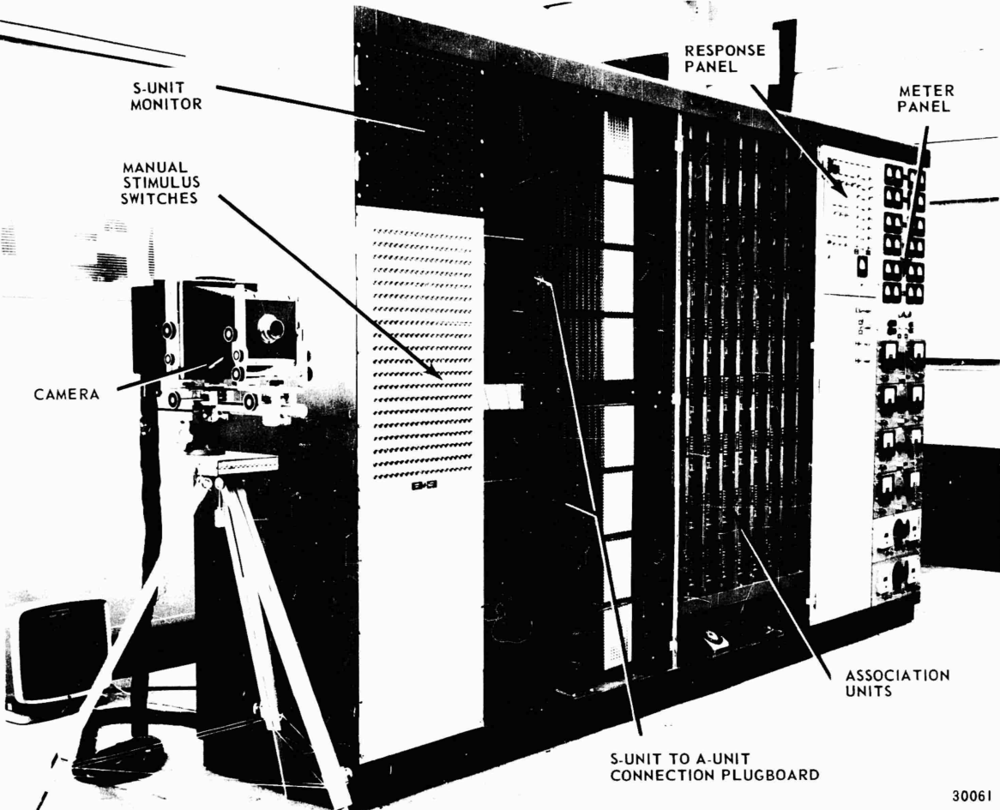
\includegraphics[height=0.40\textheight]{ch13_mark1_perceptron_1960.png}\\[1mm]
\imgcap{Mark I Perceptron, din manualul de utilizare}
\imgcredit{https://commons.wikimedia.org/wiki/File:Mark_I_Perceptron,_Figure_2_of_operator\%27s_manual.png}{Figură: J.C. Hay, A.E. Murray (1960); domeniu public; Wikimedia Commons}
\end{column}
\end{columns}
\end{frame}

\begin{frame}{Două culturi ale modelării statistice}
\itemsize{\footnotesize}
\begin{columns}[T]
\begin{column}{0.60\textwidth}
\begin{itemize}
    \item \refBreimanTC, statistician la Berkeley, descrie două culturi
    \begin{itemize}
        \item \textbf{modelarea datelor}: presupunem un model stochastic (regresia liniară $y = x^\top\beta + \varepsilon$, GARCH), îl estimăm și îi testăm parametrii
        \item \textbf{modelarea algoritmică}: tratăm mecanismul ca necunoscut; căutăm o regulă $\hat f$ care prezice bine $y$ pe date noi
    \end{itemize}
    \item Cursul a folosit prima cultură în \sfmchlink{https://danpele.github.io/SFM/RO/Cursuri/capitol2_distributii_clasice_fapte_stilizate.pdf}{capitolele 2}--\sfmchlink{https://danpele.github.io/SFM/RO/Cursuri/capitol11_piete_fractale_memorie_lunga.pdf}{11}
    \begin{itemize}
        \item acest capitol o adaugă pe a doua și analizează în ce condiții este utilă în finanțe
    \end{itemize}
\end{itemize}
\end{column}
\begin{column}{0.36\textwidth}
\centering
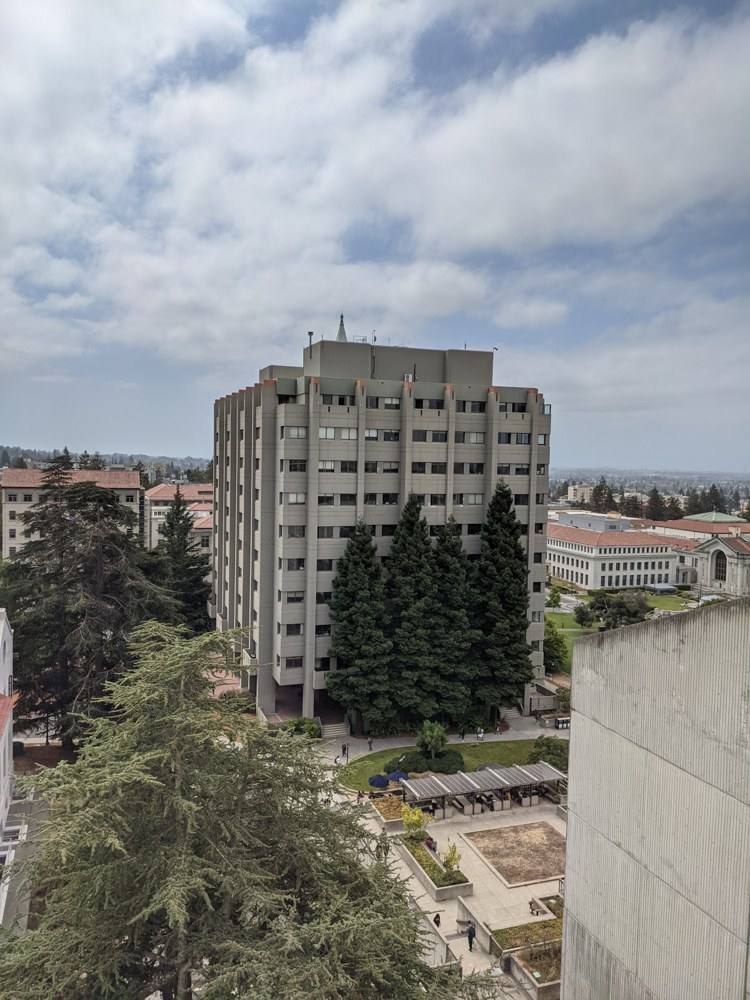
\includegraphics[height=0.46\textheight]{ch13_evans_hall_2021.jpg}\\[1mm]
\imgcap{Evans Hall, Universitatea California din Berkeley, sediul Departamentului de Statistică}
\imgcredit{https://commons.wikimedia.org/wiki/File:Evans_Hall_(UC_Berkeley).jpg}{Foto: Gabriel Classon (2021); CC BY 2.0; Wikimedia Commons}
\end{column}
\end{columns}
\end{frame}

\begin{frame}{Predicție și inferență}
\itemsize{\small}
\begin{itemize}
    \item \textbf{Inferența}: este $\beta_j \ne 0$? cît de mare este efectul? (erori standard, teste, \sfmchlink{https://danpele.github.io/SFM/RO/Cursuri/capitol6_selectia_modelului_managementul_riscului.pdf}{Capitolul 6})
    \begin{itemize}
        \item exemplu: există efectul de levier (GJR-GARCH, \sfmchlink{https://danpele.github.io/SFM/RO/Cursuri/capitol9_modele_arch_garch.pdf}{Capitolul 9})?
    \end{itemize}
    \item \textbf{Predicția}: cît de aproape este $\hat y$ de $y$ pe date pe care modelul nu le-a văzut niciodată?
    \begin{itemize}
        \item exemplu: volatilitatea săptămînii viitoare; VaR 1\% de mîine
        \item coeficienții pot fi greu de interpretat; contează eroarea pe date noi
    \end{itemize}
    \item Cele două obiective pot intra în conflict
    \begin{itemize}
        \item un estimator deplasat (ridge, lasso) poate prezice mai bine decît estimatorul nedeplasat OLS
        \item un model care prezice bine nu demonstrează un mecanism cauzal
    \end{itemize}
\end{itemize}
\end{frame}

\begin{frame}{Învățarea supervizată: notații și funcția de pierdere (1/2)}
\itemsize{\small}
\begin{itemize}
    \item Datele: perechile $(x_t, y_t)$, $t = 1, \dots, n$
    \begin{itemize}
        \item $t$: indicele observației (o zi, o săptămînă); $n$: numărul de observații
        \item $x_t \in \mathbb{R}^p$: \textbf{variabilele explicative} (features), $p$ numere cunoscute la momentul $t$ (volatilități și randamente trecute)
        \item $y_t$: \textbf{ținta} (target), mărimea pe care vrem să o prognozăm (volatilitatea săptămînii viitoare)
    \end{itemize}
    \item Două tipuri de probleme
    \begin{itemize}
        \item \textbf{regresie}: $y$ este o variabilă continuă (volatilitate, randament)
        \item \textbf{clasificare}: $y$ este o clasă (creștere/scădere, neplată; \sfmchlink{https://danpele.github.io/SFM/RO/Cursuri/capitol12_modele_scoring.pdf}{Capitolul 12})
    \end{itemize}
\end{itemize}
\end{frame}

\begin{frame}{Învățarea supervizată: notații și funcția de pierdere (2/2)}
\itemsize{\small}
\begin{itemize}
    \item Învățarea constă în alegerea regulii $\hat f$ din familia $\mathcal{F}$ care minimizează \textbf{pierderea} medie $\frac1n\sum_t L(y_t, f(x_t))$
    \begin{itemize}
        \item $f(x_t)$: prognoza dată de regula $f$ pentru observația $t$; $L(y, \hat y)$: costul prognozei $\hat y$ cînd se observă $y$
        \item $\mathcal{F}$: regulile candidate (toate regresiile liniare, toți arborii de adîncime 3); $\hat f$: regula aleasă pe baza datelor
    \end{itemize}
    \item Funcțiile de pierdere folosite în curs
    \begin{itemize}
        \item eroarea pătratică $(y - \hat y)^2$ (MSE, mean squared error); QLIKE pentru varianțe (\sfmchlink{https://danpele.github.io/SFM/RO/Cursuri/capitol8_estimatori_volatilitate.pdf}{Capitolul 8})
        \item pierderea cuantilică (pinball loss) pentru VaR (\sfmchlink{https://danpele.github.io/SFM/RO/Cursuri/capitol10_var_es_backtesting.pdf}{Capitolul 10}); log loss pentru probabilități (\sfmchlink{https://danpele.github.io/SFM/RO/Cursuri/capitol12_modele_scoring.pdf}{Capitolul 12})
    \end{itemize}
    \item Un \textbf{hiperparametru} se alege înainte de estimare
    \begin{itemize}
        \item exemple: adîncimea arborelui, penalizarea $\lambda$, numărul de neuroni
        \item parametrii (coeficienți, ponderi) se învață prin estimare
    \end{itemize}
\end{itemize}
\end{frame}

\begin{frame}{Unde ajută machine learning în finanțe și unde întîmpină dificultăți}
\itemsize{\small}
\begin{itemize}
    \item \textbf{Ajută}: ținte cu structură și cu suficiente date
    \begin{itemize}
        \item volatilitatea este persistentă (\sfmchlink{https://danpele.github.io/SFM/RO/Cursuri/capitol8_estimatori_volatilitate.pdf}{capitolele 8}--\sfmchlink{https://danpele.github.io/SFM/RO/Cursuri/capitol9_modele_arch_garch.pdf}{9}): este mult de prezis, iar efectele neliniare sînt posibile
        \item secțiuni transversale cu mii de acțiuni și multe caracteristici (studiul de caz)
    \end{itemize}
    \item \textbf{Dificultăți}: un \textbf{raport semnal--zgomot} mic
    \begin{itemize}
        \item randamentele zilnice sînt aproape imprevizibile (\sfmchlink{https://danpele.github.io/SFM/RO/Cursuri/capitol7_piete_eficiente_mers_aleator_vr.pdf}{Capitolul 7}): un model flexibil învață zgomotul
        \item piețele se schimbă (regimuri, crize): trecutul este un set de antrenare imperfect
        \item o singură istorie a prețurilor: experimentul nu poate fi repetat, iar observațiile sînt dependente
    \end{itemize}
\end{itemize}
\end{frame}

\begin{frame}{Recapitulare: contribuția machine learning}
\itemsize{\small}
\begin{itemize}
    \item Machine learning judecă un model după eroarea pe date noi, nu după semnificația coeficienților
    \item Variabile explicative $x_t$, țintă $y_t$, pierdere $L$, hiperparametri aleși înainte de estimare
    \item Finanțe: volatilitatea se prezice ușor, randamentele greu
\end{itemize}
\end{frame}


%=============================================================================
\section{Overfitting, deplasare și varianță}
%=============================================================================

\begin{frame}{Eroarea de antrenare și eroarea de test}
\itemsize{\small}
\begin{itemize}
    \item \textbf{Eroarea de antrenare}: pierderea medie pe datele folosite la estimare; \textbf{eroarea de test}: pe date noi din același proces
    \begin{itemize}
        \item eroarea de antrenare scade întotdeauna cînd modelul devine mai flexibil
    \end{itemize}
    \item \textbf{Overfitting}: modelul învață zgomotul din eșantionul de antrenare
    \begin{itemize}
        \item simptom: o eroare de antrenare mică și o eroare de test mare
        \item un arbore cu cîte o frunză pentru fiecare observație are eroare de antrenare zero, dar prognoze slabe
    \end{itemize}
    \item \textbf{Underfitting}: modelul este prea rigid pentru a surprinde semnalul
    \begin{itemize}
        \item exemplu: o prognoză constantă a volatilității într-o lume cu volatility clustering
    \end{itemize}
\end{itemize}
\end{frame}

\begin{frame}{Descompunerea deplasare--varianță (1/2)}
\itemsize{\small}
\begin{itemize}
    \item Modelul: $y = f(x) + \varepsilon$, $E[\varepsilon] = 0$, $\mathrm{Var}(\varepsilon) = \sigma^2$
    \begin{itemize}
        \item $f$: relația adevărată, necunoscută, dintre $x$ și $y$; $\varepsilon$: zgomotul, imprevizibil pe baza lui $x$, cu varianța $\sigma^2$
        \item $\hat f$: estimația lui $f$ obținută pe un eșantion de antrenare aleator; alt eșantion ar da alt $\hat f$
    \end{itemize}
    \item Eroarea de test așteptată într-un punct nou $x_0$, cu $y_0 = f(x_0) + \varepsilon_0$: \[ E\big[(y_0 - \hat f(x_0))^2\big] = \underbrace{\big(E[\hat f(x_0)] - f(x_0)\big)^2}_{\text{deplasare}^2} + \underbrace{\mathrm{Var}\big(\hat f(x_0)\big)}_{\text{varianță}} + \underbrace{\sigma^2}_{\text{zgomot}} \]
    \begin{itemize}
        \item $E[\cdot]$: media peste toate eșantioanele de antrenare posibile și peste zgomotul $\varepsilon_0$
        \item deplasarea: distanța dintre estimația medie și valoarea adevărată; varianța: cît se modifică $\hat f(x_0)$ de la un eșantion la altul
    \end{itemize}
\end{itemize}
\end{frame}

\begin{frame}{Descompunerea deplasare--varianță (2/2)}
\itemsize{\small}
\begin{itemize}
    \item Derivarea: scriem $y_0 - \hat f = (f - E\hat f) + (E\hat f - \hat f) + \varepsilon_0$, toate în punctul $x_0$
    \begin{itemize}
        \item ridicăm la pătrat și luăm media: cele trei pătrate dau deplasarea$^2$, varianța și $\sigma^2$
        \item termenii micști au media 0: $E[E\hat f - \hat f] = 0$, iar $\varepsilon_0$ este independent de eșantionul de antrenare
    \end{itemize}
    \item Interpretarea descompunerii
    \begin{itemize}
        \item un model rigid: deplasare mare, varianță mică
        \item un model flexibil: deplasare mică, varianță mare
        \item $\sigma^2$ este pragul minim: niciun model nu coboară sub el; la randamentele zilnice, $\sigma^2$ reprezintă aproape toată eroarea
    \end{itemize}
\end{itemize}
\end{frame}

\begin{frame}{Deplasarea și varianța arborilor de regresie}
\itemsize{\footnotesize}
\begin{center}
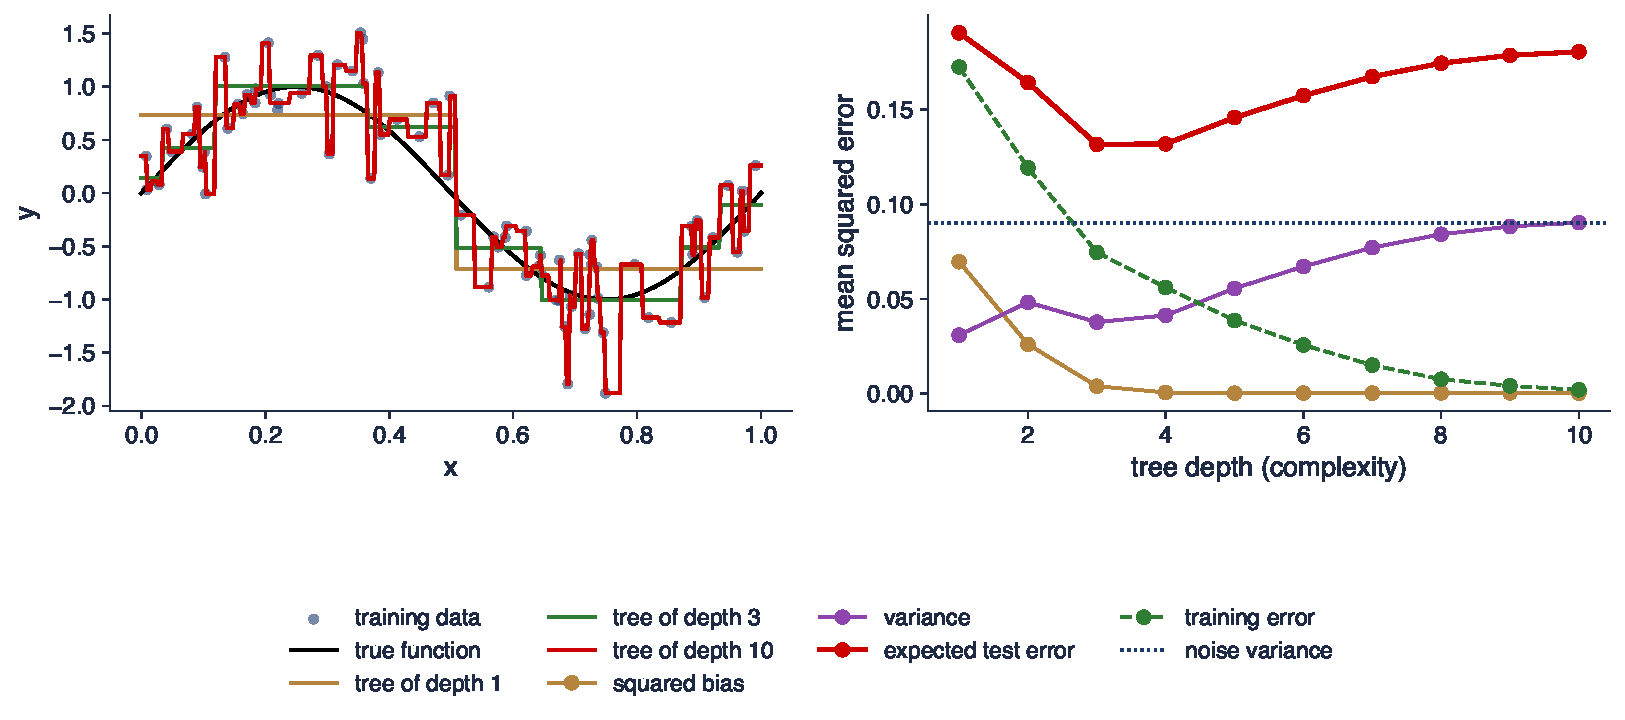
\includegraphics[width=0.97\textwidth,height=0.50\textheight,keepaspectratio]{sfm_ch13_bias_variance.pdf}
\end{center}
\vspace{-0.25cm}
\begin{itemize}
    \item Simulare: $y = \sin(2\pi x) + \varepsilon$, $\sigma^2 = 0{,}09$, $n = 80$, 300 de eșantioane de antrenare; stînga: un eșantion cu arbori de adîncime 1, 3 și 10
    \item Adîncimea 1: deplasare$^2$ $0{,}070$, varianță $0{,}031$; adîncimea 10: deplasare$^2$ $0{,}000$, varianță $0{,}090$; eroarea de test este minimă la adîncimea 3 ($0{,}132$)
\end{itemize}
\sfmquantlet{Ch_13}{SFM_ch13_validation}
\end{frame}

\begin{frame}{Interpretarea erorii de test în formă de U}
\itemsize{\small}
\begin{itemize}
    \item Eroarea de antrenare scade de la $0{,}172$ la $0{,}002$; eroarea de test scade, apoi crește
    \begin{itemize}
        \item adîncimea 10 are eroare de antrenare aproape zero și o eroare de test de $0{,}180$, mai mare decît la adîncimea 3
    \end{itemize}
    \item Consecințe practice
    \begin{itemize}
        \item nu alegeți niciodată un model după eroarea de antrenare
        \item complexitatea este un hiperparametru: se alege pe date care nu au fost folosite la estimare
        \item în finanțe zgomotul este mare, deci cel mai bun model este de obicei mai simplu decît în această simulare
    \end{itemize}
\end{itemize}
\end{frame}

\begin{frame}{Recapitulare: overfitting, deplasare și varianță}
\itemsize{\small}
\begin{itemize}
    \item Eroarea de test = deplasare$^2$ + varianță + zgomot
    \item Mai multă flexibilitate: deplasare mai mică, varianță mai mare; eroarea de antrenare este întotdeauna prea optimistă
    \item Gradul de flexibilitate se alege pe date noi
\end{itemize}
\end{frame}


%=============================================================================
\section{Validarea pentru serii de timp}
%=============================================================================

\begin{frame}{Eșantioanele de antrenare, validare și test}
\itemsize{\small}
\begin{itemize}
    \item Trei roluri pentru date
    \begin{itemize}
        \item \textbf{antrenare}: estimăm parametrii fiecărui model candidat
        \item \textbf{validare}: alegem hiperparametrii și modelul
        \item \textbf{test}: măsurăm o singură dată eroarea alegerii finale
    \end{itemize}
    \item Orice decizie luată pe baza eșantionului de test îl transformă într-un eșantion de validare
    \begin{itemize}
        \item a încerca zece modele pe datele de test și a raporta cel mai bun înseamnă selecție de model, nu testare
    \end{itemize}
    \item \textbf{Validarea încrucișată K-fold} (cross-validation): împărțim datele în $K$ părți; fiecare parte este o dată setul de validare, iar celelalte antrenează modelul
    \begin{itemize}
        \item validă pentru date i.i.d.; pentru o serie de timp doar în condiții stricte (fără dependență rămasă în erori) \refBHK
    \end{itemize}
\end{itemize}
\end{frame}

\begin{frame}{Look-ahead bias și leakage}
\itemsize{\small}
\begin{itemize}
    \item \textbf{Look-ahead bias}: prognoza pentru ziua $t$ folosește informație care nu era disponibilă la închiderea zilei $t - 1$
    \begin{itemize}
        \item variabile calculate cu prețuri viitoare (o medie mobilă centrată, o medie pe tot eșantionul)
        \item scalare sau standardizare cu statistici ale întregului eșantion; date revizuite; componența de azi a indicelui (survivorship)
    \end{itemize}
    \item \textbf{Leakage}: informația despre ținta de test ajunge în eșantionul de antrenare
    \begin{itemize}
        \item ținte suprapuse: randamentul pe 21 de zile de la ziua $t$ și cel de la ziua $t + 1$ au 20 de zile comune
        \item o partiție aleatoare pune ziua $t + 1$ în antrenare și ziua $t$ în test: modelul a văzut răspunsul
    \end{itemize}
    \item Ambele fac un model să pară mai bun decît poate fi în timp real
\end{itemize}
\end{frame}

\begin{frame}{Trei scheme de validare}
\itemsize{\footnotesize}
\begin{center}
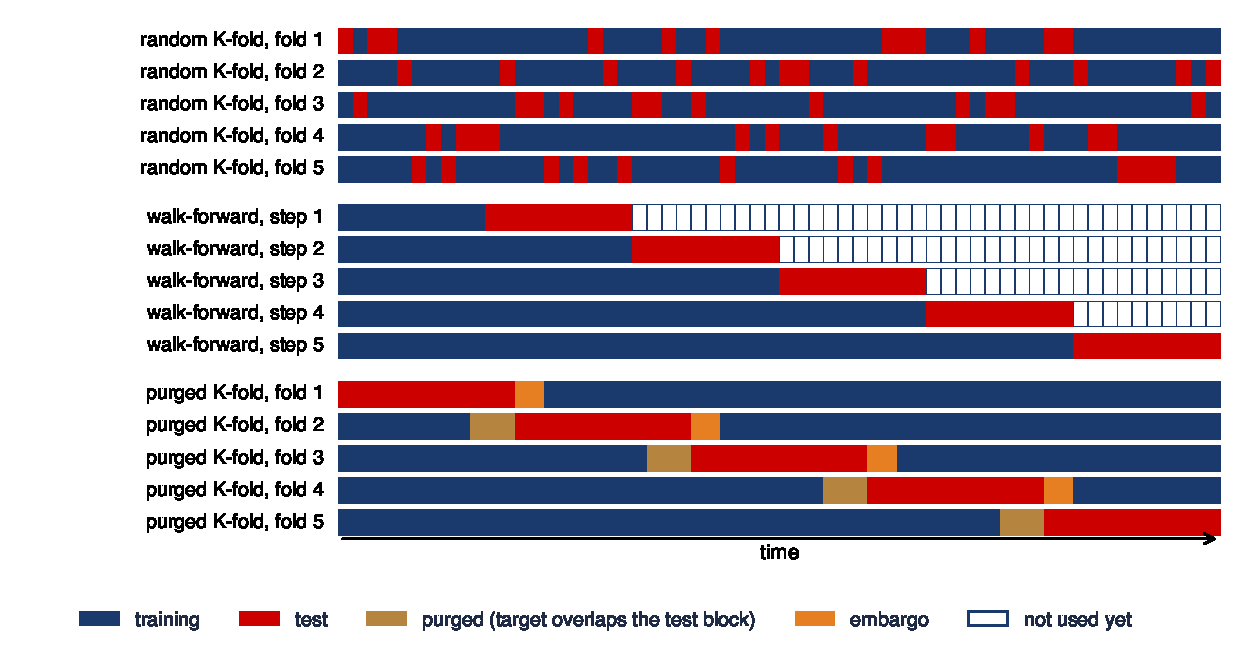
\includegraphics[width=0.97\textwidth,height=0.52\textheight,keepaspectratio]{sfm_ch13_cv_schemes.pdf}
\end{center}
\vspace{-0.25cm}
\begin{itemize}
    \item \textbf{Walk-forward}: antrenăm pe trecut, testăm pe blocul următor și avansăm; fereastra extinsă păstrează tot trecutul
    \item \textbf{K-fold cu purging și embargo} \refLdP: eliminăm rîndurile de antrenare ale căror ținte se suprapun cu blocul de test (purging) și cîteva rînduri de după el (embargo)
\end{itemize}
\sfmquantlet{Ch_13}{SFM_ch13_validation}
\end{frame}

\begin{frame}{Validarea walk-forward, pas cu pas}
\itemsize{\small}
\begin{itemize}
    \item Schema folosită în acest capitol pentru S\&P 500 (date din 8 aprilie 2008)
    \begin{itemize}
        \item cîte o partiție pentru fiecare an calendaristic din 2013: 14 partiții; modelul se reestimează în fiecare ianuarie
        \item fereastra de antrenare: toate zilele anterioare (extinsă); test: fiecare zi a anului
    \end{itemize}
    \item Purging: ținta este varianța medie din următoarele 5 zile
    \begin{itemize}
        \item pentru 2013 se elimină ultimele 5 rînduri de antrenare (de la 24 decembrie 2012): țintele lor ajung în 2013
        \item partiția pentru 2013 antrenează pe 1\,188 de zile și testează pe 252; partiția pentru 2026 antrenează pe 4\,458 de zile
    \end{itemize}
    \item În interiorul fiecărei ferestre de antrenare, hiperparametrii se aleg printr-o împărțire walk-forward doar a datelor de antrenare
    \begin{itemize}
        \item nu este nevoie de embargo: blocul de test vine întotdeauna după cel de antrenare
    \end{itemize}
\end{itemize}
\end{frame}

\begin{frame}{Leakage în practică: partiții aleatoare pe ținte suprapuse}
\itemsize{\footnotesize}
\begin{center}
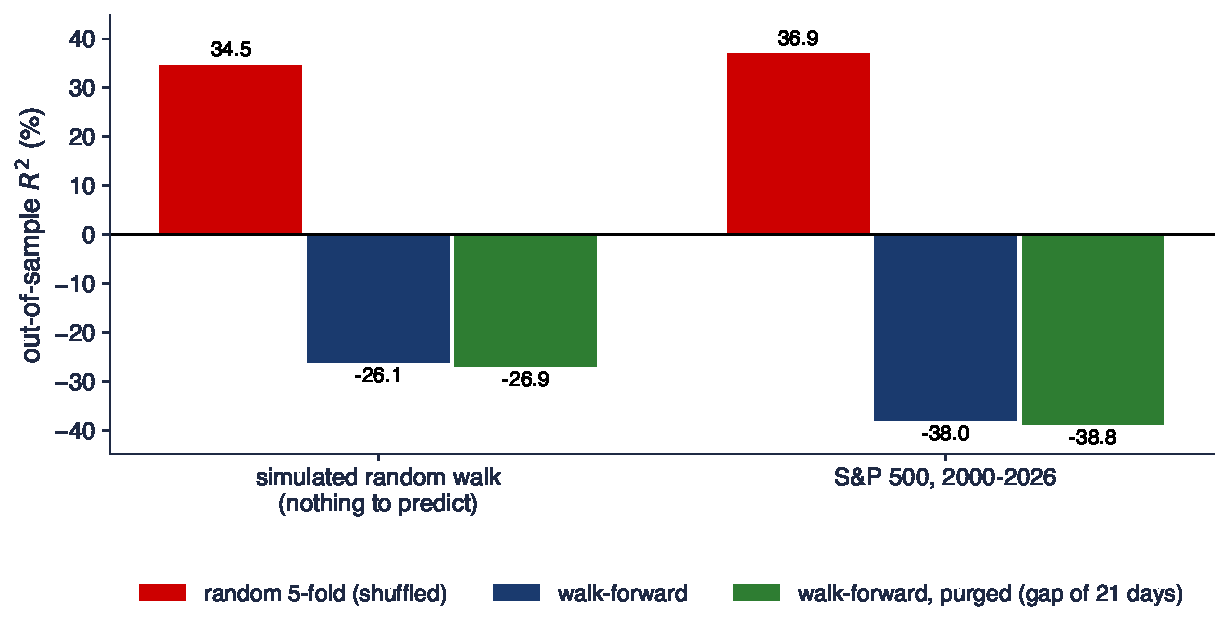
\includegraphics[width=0.97\textwidth,height=0.48\textheight,keepaspectratio]{sfm_ch13_leakage.pdf}
\end{center}
\vspace{-0.25cm}
\begin{itemize}
    \item Random forest pentru randamentul din următoarele 21 de zile, pe baza randamentelor și volatilităților trecute; $R^2$ în afara eșantionului față de media de antrenare
    \item Mers aleator simulat: 5-fold aleator $34{,}5\%$, walk-forward $-26{,}1\%$; S\&P 500 (6\,631 de zile): $36{,}9\%$ și $-38{,}0\%$
\end{itemize}
\sfmquantlet{Ch_13}{SFM_ch13_validation}
\end{frame}

\begin{frame}{Interpretare: o prognoză a zgomotului pur cu $R^2 > 30\%$}
\itemsize{\small}
\begin{itemize}
    \item Mersul aleator nu are nimic de prezis, totuși partițiile aleatoare raportează $R^2 = 34{,}5\%$
    \begin{itemize}
        \item random forest memorează zilele vecine, ale căror ținte au 20 din 21 de randamente comune cu ziua de test
    \end{itemize}
    \item Walk-forward dă un $R^2$ negativ: random forest învață zgomotul și este inferior mediei de antrenare
    \begin{itemize}
        \item purging-ul (eliminarea a 21 de zile) schimbă puțin rezultatul, deoarece în walk-forward doar rîndurile de la graniță se suprapun
    \end{itemize}
    \item Regulă: cu ținte suprapuse sau date dependente, nu amestecați niciodată ordinea temporală
\end{itemize}
\end{frame}

\begin{frame}{Recapitulare: validarea pentru serii de timp}
\itemsize{\small}
\begin{itemize}
    \item Antrenarea, validarea și testul au roluri diferite; eșantionul de test se folosește o singură dată
    \item Walk-forward cu purging respectă ordinea timpului; K-fold aleator produce leakage atunci cînd țintele se suprapun
    \item Look-ahead bias și leakage-ul produc rezultate impresionante, dar inutile
\end{itemize}
\end{frame}


%=============================================================================
\section{Regresia penalizată: ridge și lasso}
%=============================================================================

\begin{frame}{Multe variabile explicative, OLS instabil}
\itemsize{\small}
\begin{itemize}
    \item OLS (ordinary least squares, metoda celor mai mici pătrate): $\hat\beta = \arg\min_\beta \sum_t (y_t - x_t^\top\beta)^2 = (X^\top X)^{-1}X^\top y$
    \begin{itemize}
        \item $X$: matricea $n \times p$ cu rîndul $t$ egal cu $x_t^\top$; $y$: vectorul țintelor; $\arg\min_\beta$: valoarea lui $\beta$ care minimizează suma
        \item nedeplasat, dar varianța lui, $\sigma^2(X^\top X)^{-1}$ ($\sigma^2$: varianța erorii), crește foarte mult cînd variabilele sînt multe sau puternic corelate
    \end{itemize}
    \item Variabilele de volatilitate sînt puternic corelate: varianța realizată de azi, din această săptămînă și din această lună
    \begin{itemize}
        \item OLS poate da coeficienți mari, de semne opuse, care se compensează în eșantion și eșuează în afara lui
    \end{itemize}
    \item \textbf{Regresia penalizată}: minimizăm eroarea pătratică plus o penalizare pentru mărimea lui $\beta$
    \begin{itemize}
        \item acceptăm o deplasare mică pentru o reducere mare a varianței (compromisul din secțiunea 2)
    \end{itemize}
\end{itemize}
\end{frame}

\begin{frame}{Regresia ridge (1/2)}
\itemsize{\small}
\begin{itemize}
    \item \refHK: minimizăm eroarea pătratică plus o penalizare a pătratelor coeficienților \[ \hat\beta^{\,ridge} = \arg\min_\beta \sum_t (y_t - x_t^\top\beta)^2 + \lambda\sum_j \beta_j^2 = (X^\top X + \lambda I)^{-1}X^\top y \]
    \item Notațiile
    \begin{itemize}
        \item $\beta_j$: coeficientul variabilei $j$; $\sum_j \beta_j^2$: termenul de penalizare, mare cînd coeficienții sînt mari
        \item $\lambda \ge 0$: intensitatea penalizării; $\lambda = 0$ dă OLS, $\lambda \to \infty$ dă $\hat\beta \to 0$
        \item $I$: matricea identitate $p \times p$
    \end{itemize}
    \item Consecința
    \begin{itemize}
        \item $X^\top X + \lambda I$ este întotdeauna inversabilă pentru $\lambda > 0$: ridge funcționează chiar și cu mai multe variabile decît observații
    \end{itemize}
\end{itemize}
\end{frame}

\begin{frame}{Regresia ridge (2/2)}
\itemsize{\small}
\begin{itemize}
    \item \textbf{O singură variabilă}, centrată (cu media 0): $S_{xx} = \sum_t x_t^2$, $S_{xy} = \sum_t x_ty_t$ \[ \hat\beta^{\,ridge} = \dfrac{S_{xy}}{S_{xx} + \lambda} = \dfrac{S_{xx}}{S_{xx} + \lambda}\,\hat\beta^{\,OLS}, \qquad \hat\beta^{\,OLS} = \dfrac{S_{xy}}{S_{xx}} \]
    \begin{itemize}
        \item factorul $S_{xx}/(S_{xx} + \lambda)$ este în $(0, 1]$: fracțiunea din coeficientul OLS păstrată de ridge
    \end{itemize}
    \item Exemplu: $S_{xx} = 100$, $S_{xy} = 30$
    \begin{itemize}
        \item OLS: $30/100 = 0{,}30$
        \item ridge cu $\lambda = 50$: $30/150 = 0{,}20$ (factor de contracție $0{,}67$)
    \end{itemize}
    \item Ridge contractă toți coeficienții spre zero, dar nu anulează niciunul exact
\end{itemize}
\end{frame}

\begin{frame}{Lasso}
\itemsize{\footnotesize}
\begin{columns}[T]
\begin{column}{0.64\textwidth}
\begin{itemize}
    \item \refTib: $\hat\beta^{\,lasso} = \arg\min_\beta \sum_t (y_t - x_t^\top\beta)^2 + \lambda\sum_j |\beta_j|$
    \begin{itemize}
        \item valoarea absolută are un punct unghiular în 0: unii coeficienți devin \textbf{exact zero} (selecția variabilelor)
    \end{itemize}
    \item O singură variabilă: \textbf{soft thresholding} (prag de contracție)
    \begin{itemize}
        \item $\hat\beta^{\,lasso} = \mathrm{sign}(S_{xy})\,\max(|S_{xy}| - \lambda/2,\, 0)/S_{xx}$
        \item $\mathrm{sign}(S_{xy})$: semnul, $+1$ sau $-1$; dacă $|S_{xy}| \le \lambda/2$, coeficientul este exact 0
        \item aceleași date, $\lambda = 20$: $(30 - 10)/100 = 0{,}20$; zero pentru $\lambda \ge 60$
    \end{itemize}
    \item În practică
    \begin{itemize}
        \item standardizăm întîi variabilele (penalizarea depinde de unitățile lor), doar cu media și abaterea standard din antrenare
        \item alegem $\lambda$ prin validare încrucișată walk-forward; elastic net combină cele două penalizări
    \end{itemize}
\end{itemize}
\end{column}
\begin{column}{0.32\textwidth}
\centering

\includegraphics[height=0.42\textheight]{ch13_tibshirani_2012.jpg}\\[1mm]
\imgcap{Robert Tibshirani, Universitatea Stanford}
\imgcredit{https://commons.wikimedia.org/wiki/File:Robert_tibshirani.jpg}{Foto: R. Tibshirani (2012); CC BY-SA 3.0; Wikimedia Commons}
\end{column}
\end{columns}
\end{frame}

\begin{frame}{Traiectoriile ridge și lasso pentru variabilele de volatilitate}
\itemsize{\footnotesize}
\begin{center}
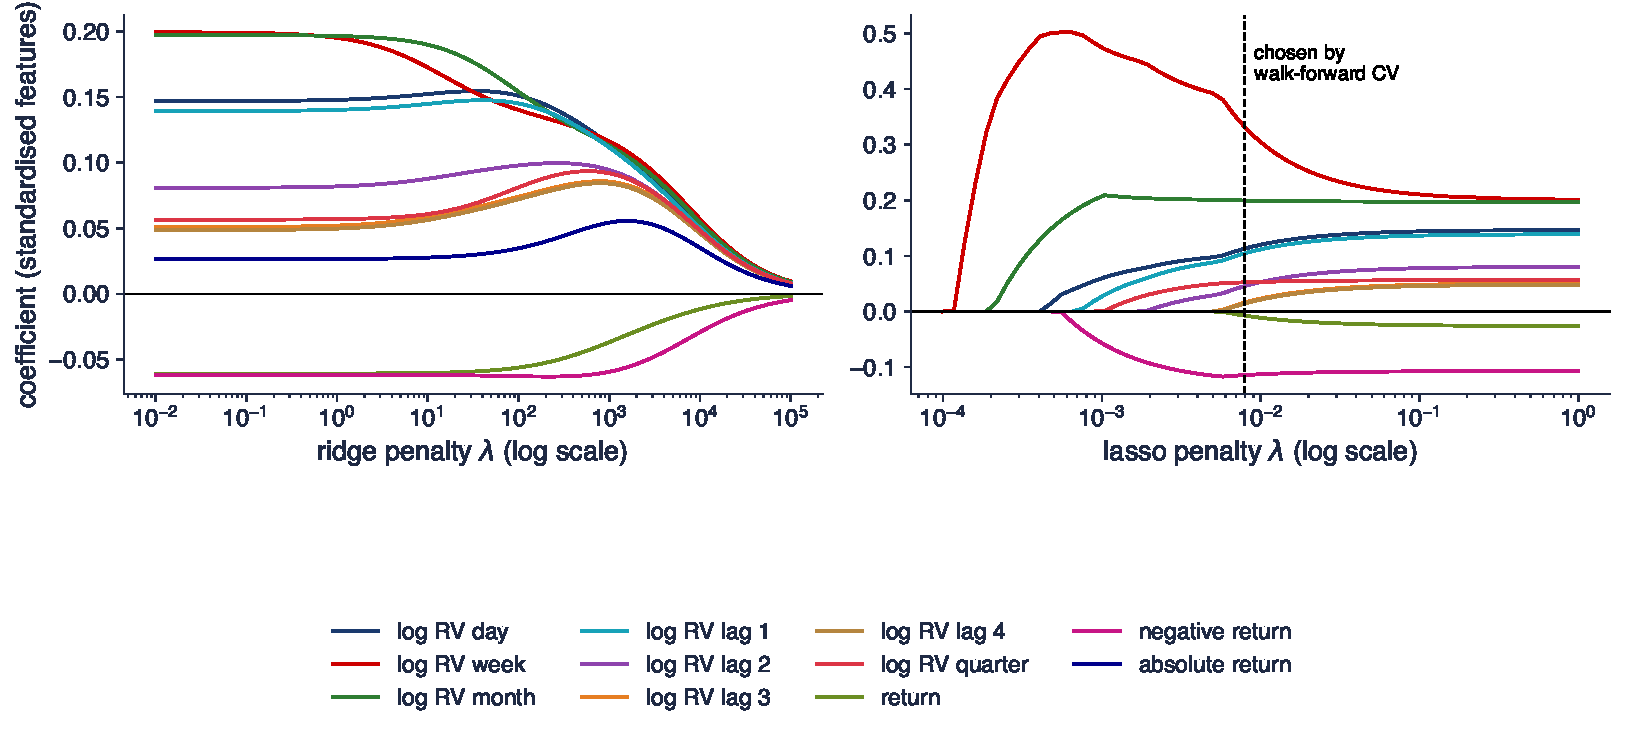
\includegraphics[width=0.97\textwidth,height=0.50\textheight,keepaspectratio]{sfm_ch13_shrinkage.pdf}
\end{center}
\vspace{-0.25cm}
\begin{itemize}
    \item Ținta: logaritmul mediei variabilei proxy a varianței din următoarele 5 zile, S\&P 500, 2008--2012 (1\,193 de zile); 11 variabile standardizate (secțiunea 7)
    \item Lasso cu $\lambda = 0{,}0079$ (CV walk-forward): rămîn 10 din 11 variabile; coeficientul săptămînal crește de la $+0{,}199$ (OLS) la $+0{,}283$, iar randamentul absolut iese din model
\end{itemize}
\sfmquantlet{Ch_13}{SFM_ch13_shrinkage_trees}
\end{frame}

\begin{frame}{Interpretarea traiectoriilor}
\itemsize{\small}
\begin{itemize}
    \item Ridge (stînga): toți coeficienții se contractă lin și împreună; variabilele corelate își împart ponderea
    \begin{itemize}
        \item randamentul negativ își păstrează semnul negativ pînă la capăt: piețele în scădere cresc volatilitatea viitoare (efectul de levier, \sfmchlink{https://danpele.github.io/SFM/RO/Cursuri/capitol9_modele_arch_garch.pdf}{Capitolul 9})
    \end{itemize}
    \item Lasso (dreapta): variabilele intră pe rînd pe măsură ce $\lambda$ scade
    \begin{itemize}
        \item varianța săptămînală intră prima: cea mai informativă variabilă luată singură
        \item la $\lambda$ ales, lasso păstrează structura HAR (zi, săptămînă, lună) plus randamentul negativ, $-0{,}112$
    \end{itemize}
    \item Lasso selectează, nu testează: un coeficient zero nu este un p-value
\end{itemize}
\end{frame}

\begin{frame}{Recapitulare: ridge și lasso}
\itemsize{\small}
\begin{itemize}
    \item Penalizările acceptă o deplasare mică în schimbul unei varianțe mai mici: $\lambda\sum\beta_j^2$ (ridge), $\lambda\sum|\beta_j|$ (lasso)
    \item Ridge contractă, lasso contractă și selectează; standardizăm întîi și alegem $\lambda$ prin CV walk-forward
    \item Pentru volatilitate, modelul penalizat păstrează structura HAR și efectul de levier
\end{itemize}
\end{frame}


%=============================================================================
\section{Arbori de decizie, random forest și gradient boosting}
%=============================================================================

\begin{frame}{Arborii de regresie}
\itemsize{\small}
\begin{itemize}
    \item Un \textbf{arbore de regresie} împarte spațiul variabilelor în dreptunghiuri și prezice media lui $y$ în fiecare \textbf{frunză}
    \begin{itemize}
        \item regula de împărțire: o variabilă $j$ și un prag $s$: stînga $x_j \le s$, dreapta $x_j > s$
    \end{itemize}
    \item \textbf{Estimarea greedy}: în fiecare nod alegem $(j, s)$ care minimizează $\mathrm{SSE} = \sum_{\text{stînga}}(y - \bar y_L)^2 + \sum_{\text{dreapta}}(y - \bar y_R)^2$
    \begin{itemize}
        \item SSE: suma pătratelor erorilor; $\bar y_L$, $\bar y_R$: mediile lui $y$ în grupul din stînga și în cel din dreapta (cele două prognoze)
        \item repetăm în fiecare jumătate pînă la o regulă de oprire: adîncimea maximă, numărul minim de observații dintr-o frunză
    \end{itemize}
    \item Puncte tari și puncte slabe
    \begin{itemize}
        \item efecte neliniare și interacțiuni fără a le specifica; insensibil la transformările monotone ale lui $x$
        \item varianță mare: o mică schimbare a datelor poate schimba tot arborele (secțiunea 2)
    \end{itemize}
\end{itemize}
\end{frame}

\begin{frame}{Exemplu rezolvat: o împărțire, pas cu pas}
\itemsize{\footnotesize}
\begin{columns}[T]
\begin{column}{0.42\textwidth}
\begin{center}
\footnotesize
\begin{tabular}{rrrr}
\toprule
$s$ & $\bar y_L$ & $\bar y_R$ & SSE \\
\midrule
$0{,}70$ & $0{,}70$ & $1{,}52$ & $1{,}708$ \\
$0{,}90$ & $0{,}80$ & $1{,}68$ & $1{,}248$ \\
$1{,}25$ & $0{,}80$ & $1{,}97$ & $0{,}227$ \\
$1{,}75$ & $1{,}00$ & $2{,}15$ & $0{,}505$ \\
$2{,}20$ & $1{,}22$ & $2{,}20$ & $1{,}468$ \\
\bottomrule
\end{tabular}
\end{center}

\end{column}
\begin{column}{0.56\textwidth}
\begin{itemize}
    \item Șase săptămîni: $x$ = volatilitatea din această săptămînă (\%), $y$ = cea din săptămîna următoare
    \begin{itemize}
        \item $x$: 0,6; 0,8; 1,0; 1,5; 2,0; 2,4; $y$: 0,7; 0,9; 0,8; 1,6; 2,1; 2,2
        \item fără împărțire: $\bar y = 1{,}38$, SSE $= 2{,}268$
    \end{itemize}
    \item Candidați: mijloacele intervalelor dintre valorile consecutive ale lui $x$
    \begin{itemize}
        \item cea mai bună împărțire $s = 1{,}25$: frunzele $0{,}80$ și $1{,}97$, SSE $= 0{,}227$
        \item o singură împărțire explică $1 - 0{,}227/2{,}268 = 0{,}90$ din variație
    \end{itemize}
\end{itemize}
\end{column}
\end{columns}
\end{frame}

\begin{frame}{Un arbore de adîncime 2 pentru volatilitatea săptămînii viitoare}
\itemsize{\footnotesize}
\begin{center}
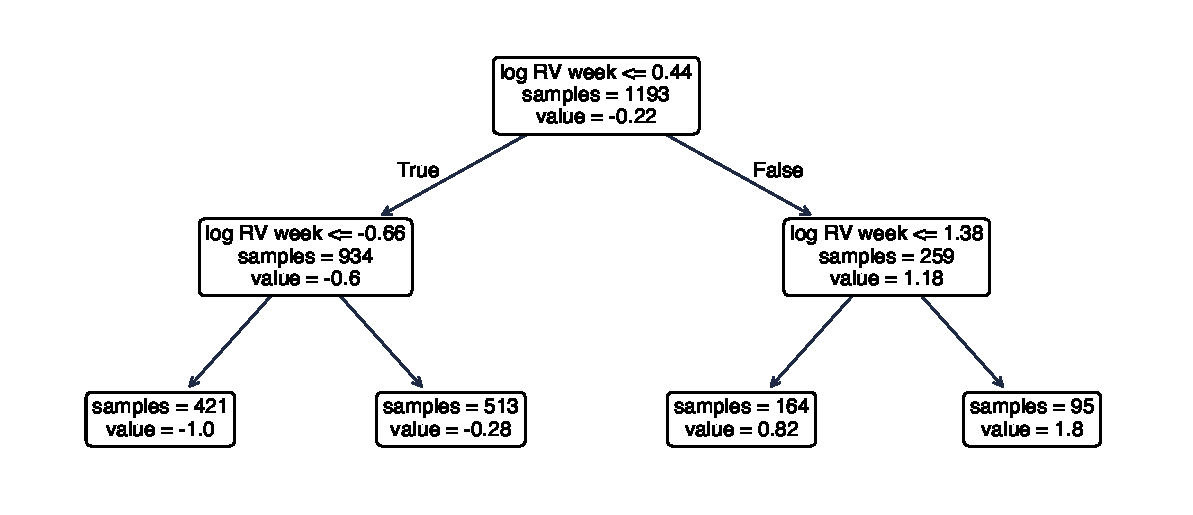
\includegraphics[width=0.97\textwidth,height=0.50\textheight,keepaspectratio]{sfm_ch13_tree.pdf}
\end{center}
\vspace{-0.25cm}
\begin{itemize}
    \item S\&P 500, 2008--2012, ținta și variabilele în logaritmul varianței (\%$^2$ pe zi); \emph{value}: media țintei în nod
    \item Interpretare: prima împărțire, log RV săptămînal $\le 0{,}44$, corespunde unei volatilități anuale de circa 19{,}8\%; toate împărțirile folosesc varianța săptămînală, variabila aleasă prima de lasso
\end{itemize}
\sfmquantlet{Ch_13}{SFM_ch13_shrinkage_trees}
\end{frame}

\begin{frame}{Random forest}
\itemsize{\small}
\begin{itemize}
    \item \refBreiman: media a $B$ arbori adînci, fiecare crescut pe un eșantion bootstrap (\sfmchlink{https://danpele.github.io/SFM/RO/Cursuri/capitol2_distributii_clasice_fapte_stilizate.pdf}{Capitolul 2}) din datele de antrenare (\textbf{bagging})
    \begin{itemize}
        \item la fiecare împărțire se încearcă doar o submulțime aleatoare de variabile: arborii devin mai puțin corelați
    \end{itemize}
    \item Efectul mediei: $B$ arbori, fiecare cu varianța $\sigma^2$ și corelația $\rho$ între oricare doi
    \begin{itemize}
        \item $\mathrm{Var}(\text{media}) = \rho\sigma^2 + (1 - \rho)\sigma^2/B$: partea $\rho\sigma^2$, comună tuturor arborilor, nu scade cu $B$
        \item cu $\rho = 0{,}3$, $\sigma^2 = 1$: $B = 1$: $1{,}000$; $B = 10$: $0{,}370$; $B = 300$: $0{,}302$
        \item mai mulți arbori nu produc overfitting; arborii mai puțin corelați (mai puține variabile la o împărțire) coboară pragul $\rho\sigma^2$
    \end{itemize}
    \item Hiperparametrii folosiți aici: 300 de arbori, cel puțin 20 de observații într-o frunză, jumătate din variabile încercate la fiecare împărțire
\end{itemize}
\end{frame}

\begin{frame}{Gradient boosting}
\itemsize{\small}
\begin{itemize}
    \item \refFriedman: construim modelul pas cu pas, fiecare arbore mic nou învățînd ce au ratat cei anteriori
    \begin{itemize}
        \item pornim de la $F_0 = \bar y$; la pasul $m$ estimăm un arbore mic $h_m$ pe reziduurile $y_t - F_{m-1}(x_t)$
        \item actualizăm $F_m = F_{m-1} + \nu\, h_m$, cu \textbf{rata de învățare} $0 < \nu \le 1$
        \item pentru pierderea pătratică, reziduurile sînt minus gradientul pierderii: de aici numele
    \end{itemize}
    \item Random forest comparat cu boosting
    \begin{itemize}
        \item random forest: arbori adînci în paralel; media reduce varianța
        \item boosting: arbori mici în secvență; fiecare pas reduce deplasarea; prea mulți pași produc overfitting
    \end{itemize}
    \item Funcționează orice pierdere derivabilă: pierderea cuantilică dă quantile boosting (secțiunea 9)
\end{itemize}
\end{frame}

\begin{frame}{Un arbore, un random forest și boosting pe date de volatilitate}
\itemsize{\footnotesize}
\begin{center}
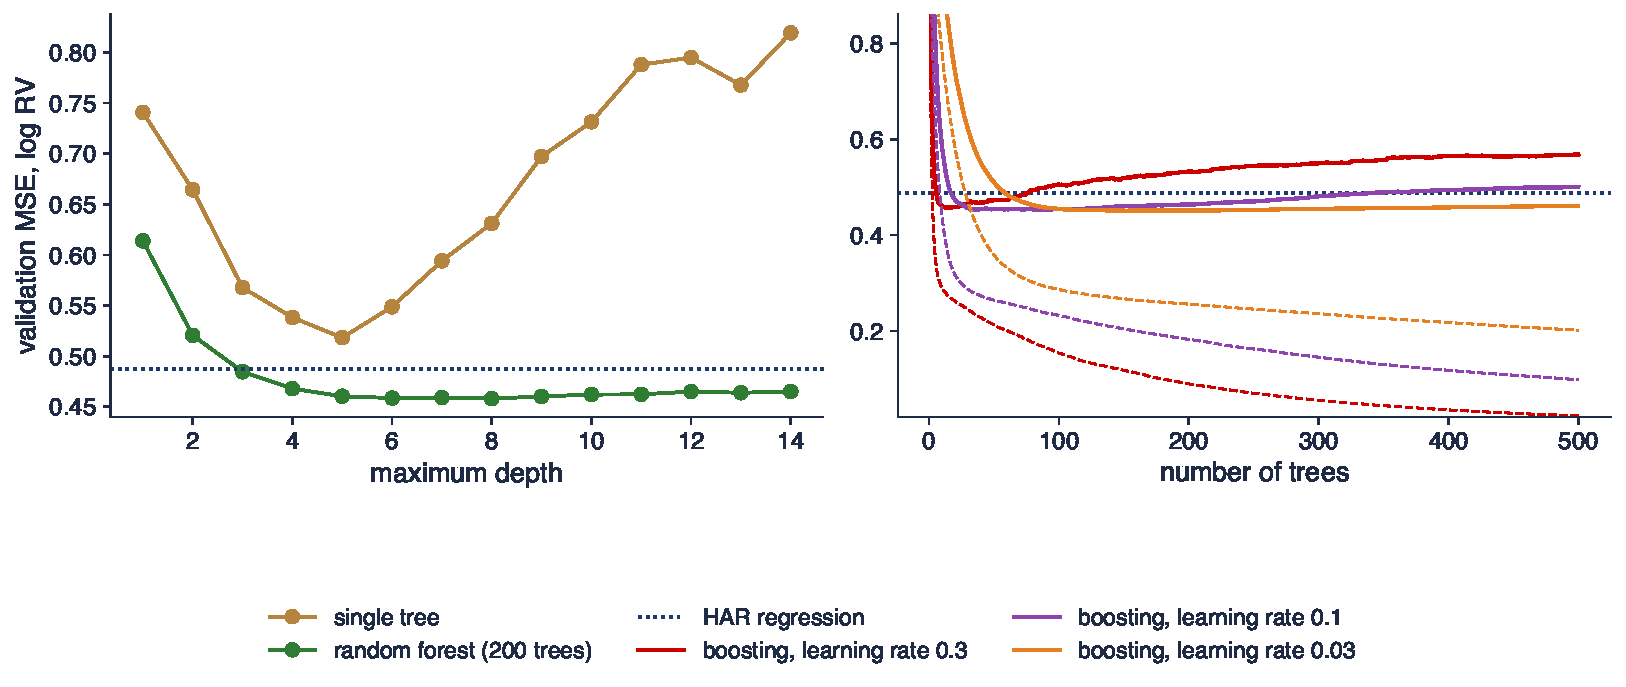
\includegraphics[width=0.97\textwidth,height=0.48\textheight,keepaspectratio]{sfm_ch13_ensembles.pdf}
\end{center}
\vspace{-0.25cm}
\begin{itemize}
    \item S\&P 500, antrenare 2008--2018 (2\,698 de zile), validare 2019--2022 (1\,008 de zile); linii întrerupte în dreapta: MSE de antrenare; punctat: regresia HAR ($0{,}487$)
    \item Un singur arbore: minimul $0{,}518$ la adîncimea 5, $0{,}819$ la adîncimea 14; random forest: $0{,}458$ (adîncimea 8) și tot $0{,}465$ la adîncimea 14
\end{itemize}
\sfmquantlet{Ch_13}{SFM_ch13_shrinkage_trees}
\end{frame}

\begin{frame}{Interpretare: media și oprirea timpurie}
\itemsize{\small}
\begin{itemize}
    \item Arborele singur intră repede în overfitting; random forest este aproape insensibil la adîncime
    \begin{itemize}
        \item media elimină cea mai mare parte din varianța arborilor adînci; random forest depășește HAR în această perioadă de validare
    \end{itemize}
    \item Boosting: eroarea de validare atinge un minim, apoi crește, în timp ce eroarea de antrenare continuă să scadă
    \begin{itemize}
        \item rata de învățare 0,3: minimul $0{,}457$ după 13 arbori, $0{,}568$ după 500 de arbori
        \item rata de învățare 0,03: minimul $0{,}451$ după 154 de arbori, $0{,}461$ după 500 de arbori: pașii mici sînt mai siguri
    \end{itemize}
    \item Numărul de arbori din boosting este un hiperparametru; numărul de arbori dintr-un random forest nu este
\end{itemize}
\end{frame}

\begin{frame}{Recapitulare: arbori și ansambluri}
\itemsize{\small}
\begin{itemize}
    \item Un arbore împarte greedy pentru a minimiza SSE; singur are varianță mare
    \item Random forest face media unor arbori adînci decorelați; boosting adaugă arbori mici estimați pe reziduuri
    \item Random forest: robust la hiperparametri; boosting: are nevoie de o rată de învățare mică și de un număr de arbori validat
\end{itemize}
\end{frame}


%=============================================================================
\section{Rețele neuronale}
%=============================================================================

\begin{frame}{De la perceptron la perceptronul multistrat (1/2)}
\itemsize{\small}
\begin{itemize}
    \item Un \textbf{neuron}: $h = g(b + w^\top x)$, o sumă ponderată a intrărilor trecută printr-o \textbf{funcție de activare} $g$
    \begin{itemize}
        \item $x$: intrările; $w$: ponderile lor; $b$: o constantă (termenul liber al neuronului); $h$: ieșirea neuronului
        \item $g$: o funcție neliniară fixată; fără ea, o rețea de neuroni ar fi doar o regresie liniară
    \end{itemize}
    \item Funcțiile de activare
    \begin{itemize}
        \item perceptronul folosește o funcție treaptă (0 sau 1)
        \item rețelele moderne folosesc funcții $g$ netede sau liniare pe porțiuni: logistică $1/(1 + e^{-z})$, tanh, ReLU $\max(0, z)$
    \end{itemize}
\end{itemize}
\end{frame}

\begin{frame}{De la perceptron la perceptronul multistrat (2/2)}
\itemsize{\small}
\begin{itemize}
    \item \textbf{MLP} (multilayer perceptron, perceptron multistrat) cu un strat ascuns de $K$ neuroni \[ \hat y = c + \sum_{k=1}^{K} v_k\, g(b_k + w_k^\top x) \]
    \begin{itemize}
        \item $w_k$, $b_k$: ponderile și constanta neuronului ascuns $k$; $v_k$: ponderea neuronului $k$ în ieșire; $c$: constanta ieșirii
        \item interpretarea: un model liniar în $K$ variabile neliniare $g(b_k + w_k^\top x)$, învățate și ele din date
    \end{itemize}
    \item Numărul de parametri pentru 11 intrări și 16 neuroni
    \begin{itemize}
        \item stratul ascuns: $11 \times 16$ ponderi $+ 16$ constante $= 192$; ieșirea: $16 + 1 = 17$; în total 209
    \end{itemize}
    \item \textbf{Aproximarea universală} \refHSW: cu suficienți neuroni, un singur strat ascuns aproximează orice funcție continuă pe o mulțime compactă
\end{itemize}
\end{frame}

\begin{frame}{O rețea mică și funcțiile ei de activare}
\itemsize{\footnotesize}
\begin{center}
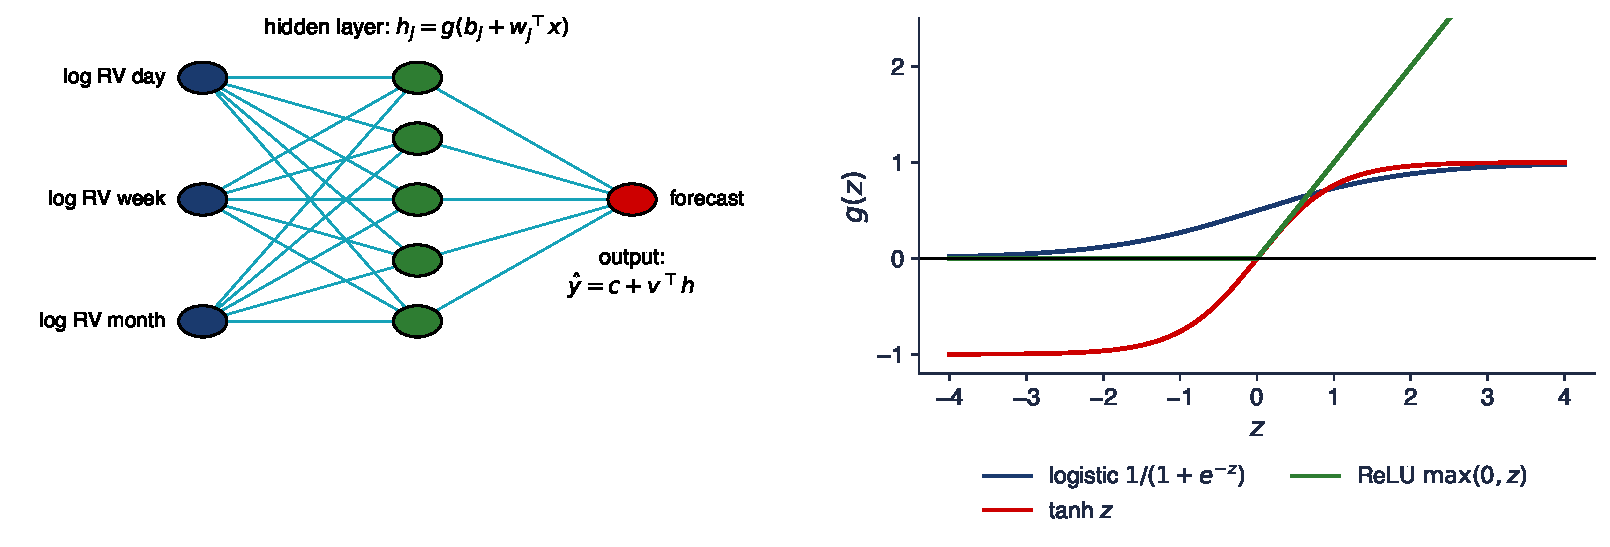
\includegraphics[width=0.97\textwidth,height=0.50\textheight,keepaspectratio]{sfm_ch13_mlp.pdf}
\end{center}
\vspace{-0.25cm}
\begin{itemize}
    \item Stînga: trei intrări HAR, cinci neuroni ascunși, o prognoză; fiecare linie este o pondere
    \item Dreapta: funcțiile logistică și tanh se saturează pentru $|z|$ mare; ReLU $= \max(0, z)$ este liniară pentru $z > 0$ și se antrenează mai repede
\end{itemize}
\sfmquantlet{Ch_13}{SFM_ch13_neural_networks}
\end{frame}

\begin{frame}{Antrenarea unei rețele}
\itemsize{\small}
\begin{itemize}
    \item Minimizăm pierderea prin \textbf{coborîre pe gradient}: $\theta \leftarrow \theta - \eta\,\nabla_\theta L$
    \begin{itemize}
        \item $\theta$: toate ponderile și constantele; $\nabla_\theta L$: gradientul, vectorul derivatelor parțiale ale pierderii; $\eta > 0$: rata de învățare (mărimea pasului)
        \item fiecare pas deplasează $\theta$ în direcția în care pierderea scade cel mai repede
        \item \textbf{retropropagarea} calculează $\nabla_\theta L$ strat cu strat, cu regula de derivare a funcțiilor compuse \refRHW
        \item o \textbf{epocă} = o trecere prin datele de antrenare; Adam este o metodă de gradient cu pași adaptivi
    \end{itemize}
    \item Pierderea nu este convexă: ponderi inițiale diferite dau rețele diferite
    \begin{itemize}
        \item fixăm semințele aleatoare și facem media a cinci rețele (un \textbf{ansamblu})
    \end{itemize}
    \item Împotriva overfitting-ului
    \begin{itemize}
        \item standardizăm intrările și ținta cu statisticile de antrenare; o penalizare $L_2$ a ponderilor (ca la ridge); un număr fix de epoci
        \item date puține, rețea mică: aici este suficient un strat ascuns cu 16 neuroni
    \end{itemize}
\end{itemize}
\end{frame}

\begin{frame}{De la Deep Blue la deep learning}
\itemsize{\footnotesize}
\begin{columns}[T]
\begin{column}{0.48\textwidth}
\centering
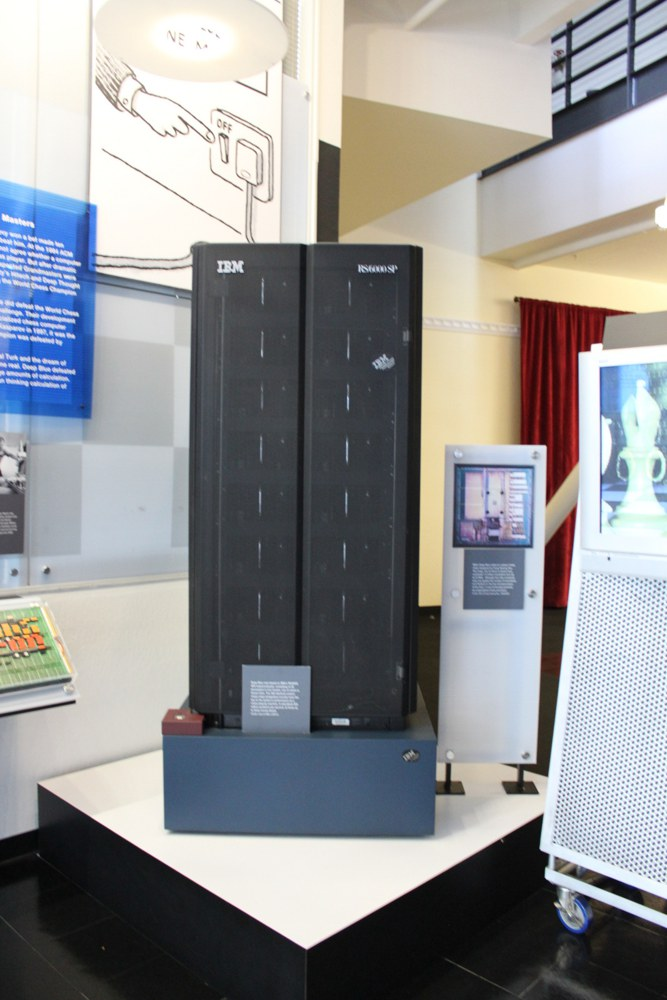
\includegraphics[height=0.36\textheight]{ch13_deep_blue_2011.jpg}\\[1mm]
\imgcap{IBM Deep Blue, Computer History Museum}
\imgcredit{https://commons.wikimedia.org/wiki/File:IBM_Deep_Blue_at_Computer_History_Museum_(9361685537).jpg}{Foto: Anton Chiang (2011); CC BY 2.0; Wikimedia Commons}
\end{column}
\begin{column}{0.48\textwidth}
\centering
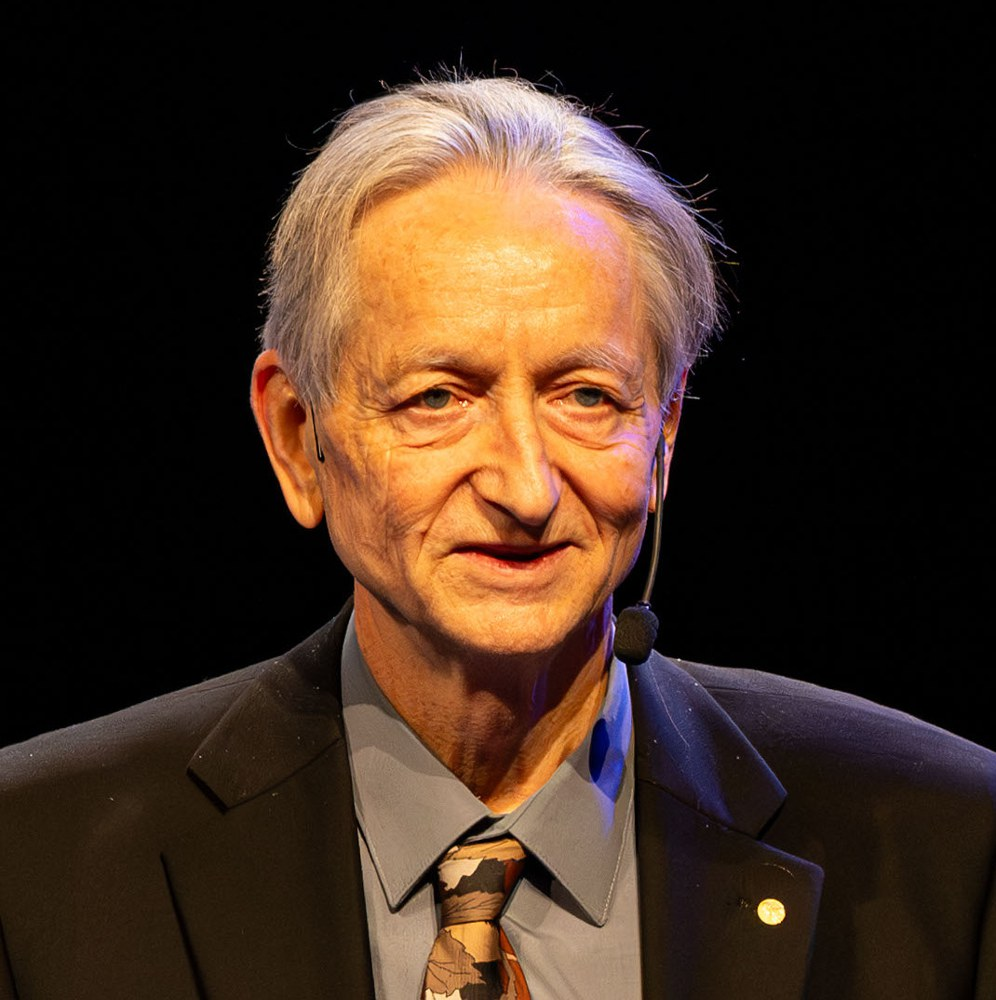
\includegraphics[height=0.36\textheight]{ch13_hinton_2024.jpg}\\[1mm]
\imgcap{Geoffrey Hinton, Premiul Nobel pentru fizică 2024}
\imgcredit{https://commons.wikimedia.org/wiki/File:Geoffrey_E._Hinton,_2024_Nobel_Prize_Laureate_in_Physics_(cropped1).jpg}{Foto: Arthur Petron (2024); CC BY-SA 4.0; Wikimedia Commons}
\end{column}
\end{columns}\begin{itemize}
    \item 1997: Deep Blue l-a învins pe campionul mondial la șah mai ales prin căutare și reguli de evaluare scrise de oameni, nu prin învățare din date
    \item Deep learning (multe straturi, volume uriașe de date) domină azi imaginile și textul; la prețurile financiare datele sînt puține și zgomotoase, deci rețelele mici sînt regula
\end{itemize}
\end{frame}

\begin{frame}{ARCH cu rețea neuronală: modelul din manual (1/2)}
\itemsize{\small}
\begin{itemize}
    \item \refFHH, cap.~19: $r_t = f(x_{t-1}) + s(x_{t-1})\,\varepsilon_t$, cu $f$ și $s^2$ estimate prin rețele neuronale
    \begin{itemize}
        \item $r_t$: randamentul zilei $t$; $x_{t-1}$: intrările cunoscute la închiderea zilei $t - 1$
        \item $f(x_{t-1})$: media condiționată; $s^2(x_{t-1})$: varianța condiționată; $\varepsilon_t$: un șoc cu media 0 și varianța 1
    \end{itemize}
    \item ARCH (\refEngle) este cazul particular $s^2(x) = \omega + \sum_i \alpha_i r_{t-i}^2$
    \begin{itemize}
        \item $\omega > 0$, $\alpha_i \ge 0$: varianța este o funcție liniară de pătratele randamentelor trecute
        \item rețeaua nu impune nicio formă funcției $s^2$
    \end{itemize}
\end{itemize}
\end{frame}

\begin{frame}{ARCH cu rețea neuronală: modelul din manual (2/2)}
\itemsize{\small}
\begin{itemize}
    \item Quantlet-ul \refSFEa: GBP/USD, intrările $x$ = ultimele 3 randamente, randamentul obligațiunilor germane pe 10 ani, randamentul aurului
    \begin{itemize}
        \item pasul 1: o rețea $\hat f$ pentru medie; reziduurile $e_t = r_t - \hat f(x_{t-1})$
        \item pasul 2: o rețea pentru $e_t^2$ dă varianța condiționată $\hat s^2(x_{t-1})$
    \end{itemize}
    \item Rețea \textbf{RBF} (radial basis function, cu funcții de bază radiale) cu 3 unități, ca în Quantlet
    \begin{itemize}
        \item unitatea $j$: $\exp(-\|x - c_j\|^2/s_j^2)$; $c_j$: centrul ei (obținut prin clustering); $s_j$: lățimea ei; $\|x - c_j\|$: distanța de la $x$ la $c_j$
        \item unitatea este aproape de 1 cînd $x$ este lîngă $c_j$ și aproape de 0 departe de el; ieșirea: o combinație liniară a celor 3 unități
        \item nimic nu impune $\hat s^2 > 0$: o rețea pentru varianță are nevoie de un prag minim, pe care GARCH îl garantează prin restricțiile sale
    \end{itemize}
\end{itemize}
\end{frame}

\begin{frame}{ARCH cu rețea neuronală pentru GBP/USD}
\itemsize{\footnotesize}
\begin{center}
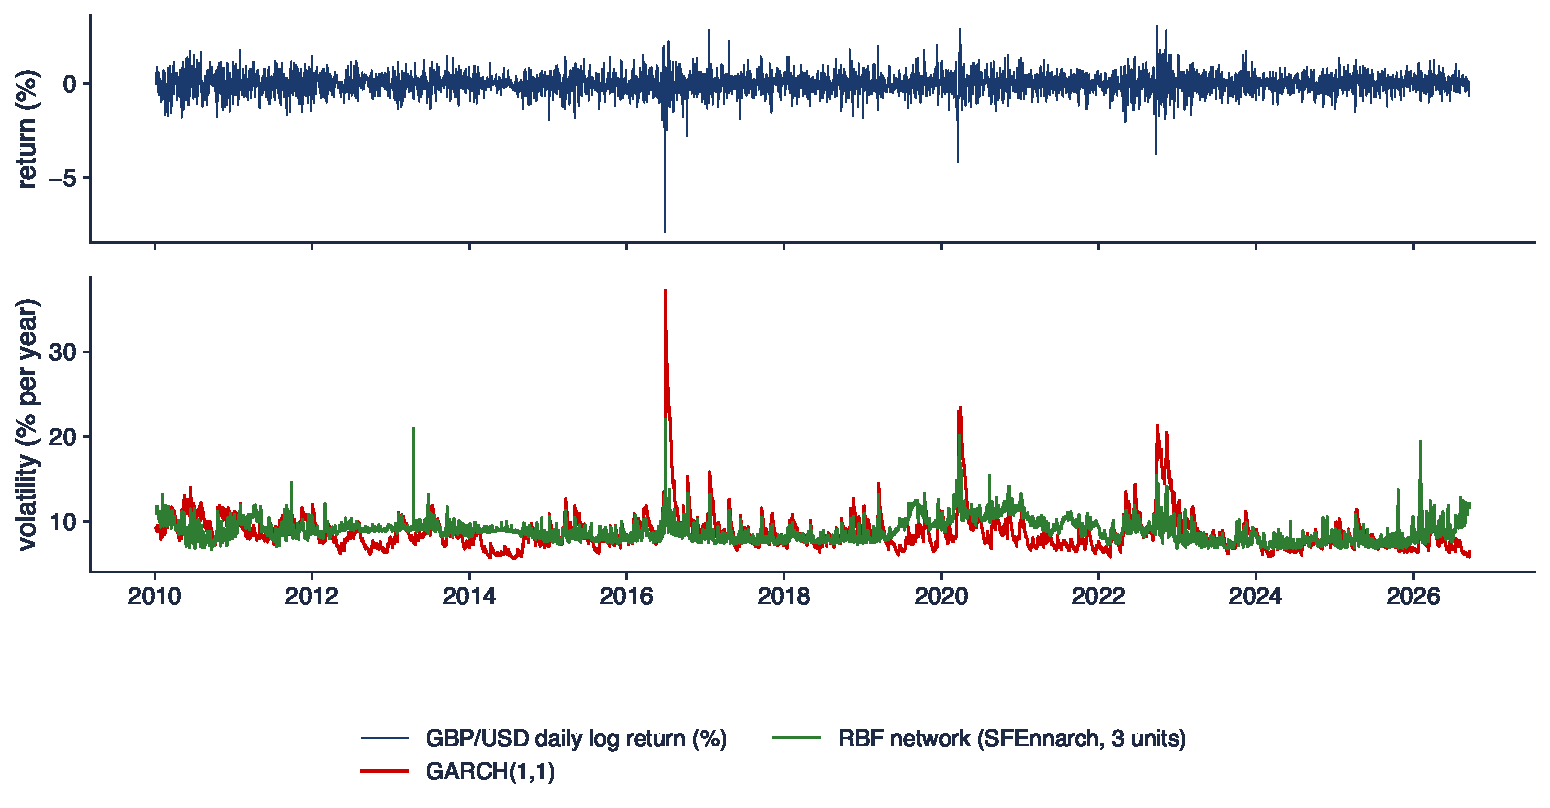
\includegraphics[width=0.97\textwidth,height=0.50\textheight,keepaspectratio]{sfm_ch13_nnarch.pdf}
\end{center}
\vspace{-0.25cm}
\begin{itemize}
    \item Date zilnice din 7 ianuarie 2010 (4\,048 de zile); volatilitatea anualizată a rețelei RBF și a modelului GARCH(1,1) ($\hat\alpha = 0{,}077$, $\hat\beta = 0{,}892$)
    \item Volatilitatea medie: rețeaua 8{,}9\%, GARCH 8{,}8\%; corelația celor două traiectorii $0{,}45$ (un MLP mic: $0{,}43$)
\end{itemize}
\sfmquantlet{Ch_13}{SFM_ch13_neural_networks}
\end{frame}

\begin{frame}{Interpretare: formă flexibilă, memorie scurtă}
\itemsize{\small}
\begin{itemize}
    \item După votul pentru Brexit, GARCH atinge maximul de 37{,}3\% (28 iunie 2016); rețeaua doar 22{,}0\%
    \begin{itemize}
        \item rețeaua vede doar ultimele 3 randamente: un randament mare îi crește varianța timp de 3 zile, apoi efectul dispare
        \item GARCH transmite tot trecutul prin $\beta\,\sigma_{t-1}^2$: volatility clustering are nevoie de memorie, nu doar de flexibilitate
    \end{itemize}
    \item Rețeaua pentru medie explică $0{,}08\%$ din randamente în eșantion: cursurile de schimb sînt aproape un mers aleator
    \begin{itemize}
        \item partea utilă a modelului NN-ARCH este varianța, ca la GARCH
    \end{itemize}
    \item Lecția: variabilele bune (mediile HAR, secțiunea 7) contează mai mult decît tipul de rețea
\end{itemize}
\end{frame}

\begin{frame}{Prognoza nivelului unui curs de schimb: SFEnnjpyusd}
\itemsize{\small}
\begin{itemize}
    \item Quantlet-ul \refSFEb{} prognozează cursul yen--dolar din ultimele 3 valori, cu o rețea RBF cu 3 unități
    \begin{itemize}
        \item primele 80\% din zile pentru antrenare, ultimele 20\% pentru test; aici USD/JPY din 2000, cu separarea la 21 iunie 2021
    \end{itemize}
    \item Două capcane ale prognozei nivelului
    \begin{itemize}
        \item o serie de niveluri pare previzibilă deoarece $P_t \approx P_{t-1}$: reperul corect este mersul aleator $\hat P_t = P_{t-1}$ (\sfmchlink{https://danpele.github.io/SFM/RO/Cursuri/capitol7_piete_eficiente_mers_aleator_vr.pdf}{Capitolul 7})
        \item o rețea cu unități mărginite nu poate extrapola: nivelurile de test urcă pînă la 163{,}9, iar maximul din antrenare a fost 134{,}9
    \end{itemize}
    \item Codul original rescalează prognozele de test cu intervalul seriei de test, necunoscut în timp real; aici se folosește intervalul din antrenare
\end{itemize}
\end{frame}

\begin{frame}{Rețeaua RBF comparată cu mersul aleator}
\itemsize{\footnotesize}
\begin{center}
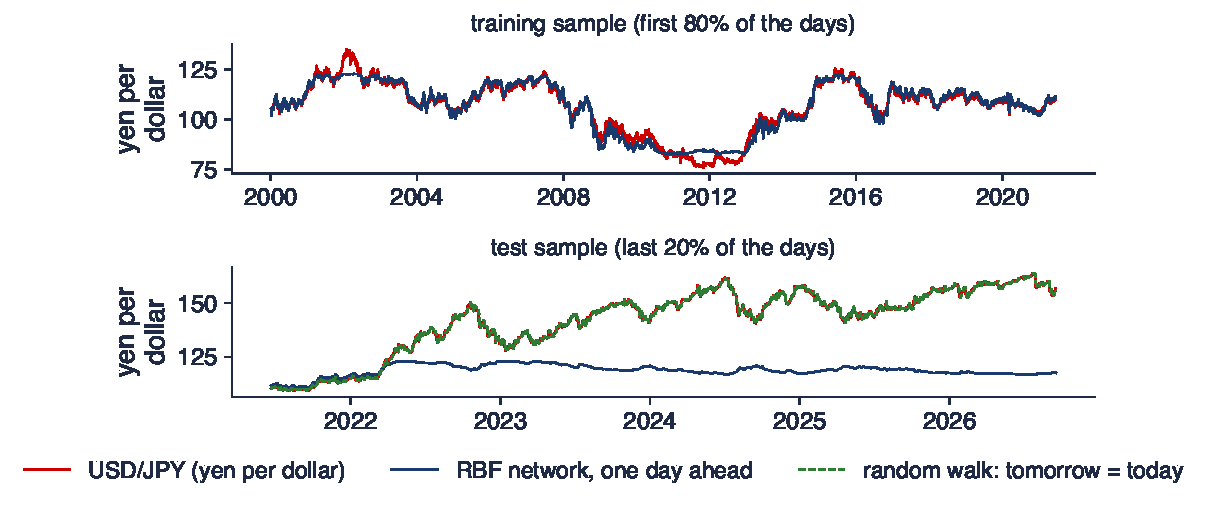
\includegraphics[width=0.97\textwidth,height=0.50\textheight,keepaspectratio]{sfm_ch13_nnjpy.pdf}
\end{center}
\vspace{-0.25cm}
\begin{itemize}
    \item RMSE (root mean squared error, rădăcina erorii pătratice medii) în yeni: antrenare: rețeaua 2{,}64, mersul aleator 0{,}66; test: rețeaua 27{,}56, mersul aleator 0{,}89
    \item Interpretare: în afara eșantionului rețeaua este de 31 de ori mai slabă decît „mîine = azi”; pe randamente, aceeași rețea are un $R^2$ în afara eșantionului de $-0{,}14\%$
\end{itemize}
\sfmquantlet{Ch_13}{SFM_ch13_neural_networks}
\end{frame}

\begin{frame}{Recapitulare: rețele neuronale}
\itemsize{\small}
\begin{itemize}
    \item Un MLP este un model liniar în variabile neliniare învățate; se antrenează prin coborîre pe gradient și retropropagare
    \item NN-ARCH: o funcție a varianței flexibilă, dar fără memoria GARCH și fără garanția pozitivității
    \item Prognozați randamente, nu niveluri, și comparați întotdeauna cu mersul aleator
\end{itemize}
\end{frame}


%=============================================================================
\section{Aplicație: prognoza volatilității realizate}
%=============================================================================

\begin{frame}{Ținta și variabilele explicative (1/2)}
\itemsize{\small}
\begin{itemize}
    \item Variabila proxy zilnică a varianței din \sfmchlink{https://danpele.github.io/SFM/RO/Cursuri/capitol8_estimatori_volatilitate.pdf}{Capitolul 8} (fără date intrazilnice): o estimație a varianței zilei $t$ din prețurile de deschidere, maxim, minim și închidere \[ v_t = o_t^2 + \tfrac12(u_t - d_t)^2 - (2\ln 2 - 1)c_t^2 \]
    \begin{itemize}
        \item $o_t$: randamentul logaritmic peste noapte (de la închiderea precedentă la deschidere)
        \item $u_t, d_t, c_t$: logaritmii maximului, minimului și închiderii față de deschidere (termenul Garman--Klass, \refGK)
    \end{itemize}
    \item \textbf{Ținta}: $y_t = \ln\big(\tfrac15\sum_{j=1}^{5} v_{t+j}\big)$, logaritmul varianței realizate din săptămîna următoare
    \begin{itemize}
        \item $j = 1, \dots, 5$: următoarele cinci zile de tranzacționare; ținta este cunoscută abia la închiderea zilei $t + 5$
        \item logaritmul apropie ținta de distribuția Normală și face prognozele pozitive după $\exp$
    \end{itemize}
\end{itemize}
\end{frame}

\begin{frame}{Ținta și variabilele explicative (2/2)}
\itemsize{\small}
\begin{itemize}
    \item \textbf{Variabilele explicative} la închiderea zilei $t$
    \begin{itemize}
        \item HAR: $\ln v_t$, logaritmul mediei pe 5 zile (săptămîna) și pe 22 de zile (luna)
        \item extinse (11): în plus 4 laguri ale lui $\ln v_t$ ($\ln v_{t-1}, \dots, \ln v_{t-4}$), media pe 66 de zile, $r_t$, $\min(r_t, 0)$, $|r_t|$
    \end{itemize}
    \item Notațiile
    \begin{itemize}
        \item $r_t$: randamentul logaritmic al zilei $t$; $|r_t|$: valoarea lui absolută
        \item $\min(r_t, 0)$: randamentul, dacă este negativ, și 0 în rest; permite scăderilor și creșterilor să aibă efecte diferite (efectul de levier)
    \end{itemize}
\end{itemize}
\end{frame}

\begin{frame}{Reperul HAR (1/2)}
\itemsize{\small}
\begin{itemize}
    \item Modelul \textbf{HAR} (heterogeneous autoregressive, autoregresiv heterogen) \refCorsi{} \[ y_t = \beta_0 + \beta_d\ln v_t + \beta_w\ln v_t^{(w)} + \beta_m\ln v_t^{(m)} + u_t \]
    \begin{itemize}
        \item $v_t^{(w)}$, $v_t^{(m)}$: media lui $v$ pe ultimele 5 zile (săptămîna) și pe ultimele 22 de zile (luna)
        \item $\beta_0$: constanta; $\beta_d, \beta_w, \beta_m$: ponderile celor trei orizonturi; $u_t$: eroarea
    \end{itemize}
    \item Interpretarea
    \begin{itemize}
        \item trei orizonturi ale participanților la piață (zilnic, săptămînal, lunar); estimat prin OLS
        \item cu ponderi pozitive pe cele trei orizonturi, un șoc al volatilității se atenuează lent
        \item un model liniar simplu care imită memoria lungă (\sfmchlink{https://danpele.github.io/SFM/RO/Cursuri/capitol11_piete_fractale_memorie_lunga.pdf}{Capitolul 11}) și este greu de depășit
    \end{itemize}
\end{itemize}
\end{frame}

\begin{frame}{Reperul HAR (2/2)}
\itemsize{\small}
\begin{itemize}
    \item Întrebarea acestei secțiuni
    \begin{itemize}
        \item adaugă lasso, random forest, gradient boosting sau un MLP ceva peste HAR în afara eșantionului?
        \item un studiu amplu cu date intrazilnice găsește cîștiguri modeste, mai ales din variabile suplimentare \refCSV
    \end{itemize}
    \item Schema de evaluare: walk-forward din secțiunea 3, reestimare anuală; S\&P 500 din 2013, Bitcoin din 2018
    \begin{itemize}
        \item prognoza varianței $\hat h_t = \exp(\hat y_t + \hat s^2/2)$, cu $\hat s^2$ varianța reziduală din antrenare (media log-Normală)
        \item $\hat y_t$: prognoza logaritmului varianței; $\exp(\hat y_t)$ singur ar subestima varianța medie, de aici termenul $\hat s^2/2$
    \end{itemize}
\end{itemize}
\end{frame}

\begin{frame}{Evaluarea (1/3): $R^2$ în afara eșantionului}
\itemsize{\small}
\begin{itemize}
    \item $R^2$ \textbf{în afara eșantionului} față de o prognoză de referință $\tilde y_t$ \refCT{} \[ R^2_{OOS} = 1 - \frac{\sum_t (y_t - \hat y_t)^2}{\sum_t (y_t - \tilde y_t)^2} \]
    \begin{itemize}
        \item $\hat y_t$: prognoza modelului; sumele se calculează doar pe zilele de test
        \item reperul $\tilde y_t$: media din antrenare sau HAR
    \end{itemize}
    \item Interpretarea
    \begin{itemize}
        \item $R^2_{OOS} \le 1$; $R^2_{OOS} > 0$: eroare pătratică mai mică decît a reperului; $R^2_{OOS} < 0$: mai slab decît reperul
        \item spre deosebire de $R^2$ din eșantion, poate fi negativ
    \end{itemize}
    \item Pas cu pas, S\&P 500, MLP față de HAR
    \begin{itemize}
        \item $1 - 0{,}397/0{,}433 = 1 - 0{,}917$, adică $+8{,}3\%$
    \end{itemize}
\end{itemize}
\end{frame}

\begin{frame}{Evaluarea (2/3): QLIKE}
\itemsize{\small}
\begin{itemize}
    \item \textbf{QLIKE} (\sfmchlink{https://danpele.github.io/SFM/RO/Cursuri/capitol8_estimatori_volatilitate.pdf}{Capitolul 8}): o funcție de pierdere pentru prognozele varianței, robustă la o variabilă proxy zgomotoasă \refPatton{} \[ L_t = \frac{\mathrm{RV}_t}{\hat h_t} + \ln\hat h_t \]
    \begin{itemize}
        \item $\mathrm{RV}_t$: varianța realizată din următoarele 5 zile (ținta, în niveluri); $\hat h_t$: prognoza ei
        \item pentru un $\mathrm{RV}_t$ dat, pierderea este minimă la $\hat h_t = \mathrm{RV}_t$; un QLIKE mediu mai mic este mai bun
    \end{itemize}
    \item Asimetria
    \begin{itemize}
        \item pentru $\mathrm{RV} = 1$: $\hat h = 0{,}5$ costă $1{,}307$, $\hat h = 2$ costă $1{,}193$
        \item subestimarea este penalizată mai mult: în managementul riscului, subestimarea volatilității este eroarea costisitoare
    \end{itemize}
\end{itemize}
\end{frame}

\begin{frame}{Evaluarea (3/3): testul Diebold--Mariano}
\itemsize{\small}
\begin{itemize}
    \item Testul \textbf{Diebold--Mariano} \refDM: au două modele $A$ și $B$ aceeași pierdere așteptată? \[ d_t = L_t^{A} - L_t^{B}, \qquad \mathrm{DM} = \frac{\bar d}{\sqrt{\widehat{\mathrm{LRV}}/n}} \sim N(0,1) \text{ la acuratețe egală} \]
    \begin{itemize}
        \item $L_t^{A}$, $L_t^{B}$: pierderile celor două modele în ziua $t$; $\bar d$: media lui $d_t$; $n$: numărul zilelor de test
        \item $\widehat{\mathrm{LRV}}$: varianța pe termen lung Newey--West a lui $d_t$ (5 laguri), deoarece țintele suprapuse fac $d_t$ autocorelat
    \end{itemize}
    \item Interpretarea
    \begin{itemize}
        \item DM $< 0$: $A$ are pierderea mai mică; DM $> 0$: $B$ este mai bun
        \item $|\mathrm{DM}| > 1{,}96$: diferența este semnificativă la 5\%
    \end{itemize}
\end{itemize}
\end{frame}

\begin{frame}{Rezultatele: S\&P 500 și Bitcoin}
\itemsize{\footnotesize}
\begin{center}
\scriptsize
\begin{tabular}{llrrrr}
\toprule
& Model & $R^2_{OOS}$ față de medie & $R^2_{OOS}$ față de HAR & QLIKE & DM față de HAR (p) \\
\midrule
S\&P 500 & HAR & $61{,}5$ & -- & $0{,}414$ & -- \\
 & Lasso & $64{,}2$ & ${+7{,}1}$ & $0{,}400$ & ${-5{,}12}$ ($<$\,0{,}001) \\
 & RF & $61{,}9$ & ${+1{,}0}$ & $0{,}416$ & ${+0{,}32}$ (0{,}747) \\
 & GB & $60{,}4$ & ${-2{,}7}$ & $0{,}421$ & ${+1{,}02}$ (0{,}308) \\
 & MLP & $64{,}7$ & ${+8{,}3}$ & $0{,}398$ & ${-3{,}96}$ ($<$\,0{,}001) \\
\midrule
Bitcoin & HAR & $44{,}0$ & -- & $3{,}111$ & -- \\
 & Lasso & $45{,}1$ & ${+2{,}0}$ & $3{,}108$ & ${-0{,}64}$ (0{,}520) \\
 & RF & $43{,}4$ & ${-1{,}2}$ & $3{,}119$ & ${+0{,}81}$ (0{,}418) \\
 & GB & $41{,}7$ & ${-4{,}2}$ & $3{,}148$ & ${+2{,}12}$ (0{,}034) \\
 & MLP & $43{,}8$ & ${-0{,}3}$ & $3{,}123$ & ${+1{,}10}$ (0{,}272) \\
\bottomrule
\end{tabular}
\end{center}
\begin{itemize}
    \item Prognoze pentru 3\,444 de zile (S\&P 500, de la 2 ianuarie 2013) și 3\,178 de zile (Bitcoin, de la 1 ianuarie 2018); $R^2_{OOS}$ în \%, pe log RV; GB: gradient boosting
    \item S\&P 500: lasso și MLP depășesc semnificativ HAR ($+7{,}1\%$; $+8{,}3\%$); random forest și boosting nu
    \item Bitcoin: niciun model nu depășește HAR; boosting este semnificativ mai slab (DM $+2{,}12$)
\end{itemize}\sfmquantlet{Ch_13}{SFM_ch13_volatility_forecast}
\end{frame}

\begin{frame}{Prognozele în două furtuni: 2020 și 2025}
\itemsize{\footnotesize}
\begin{center}
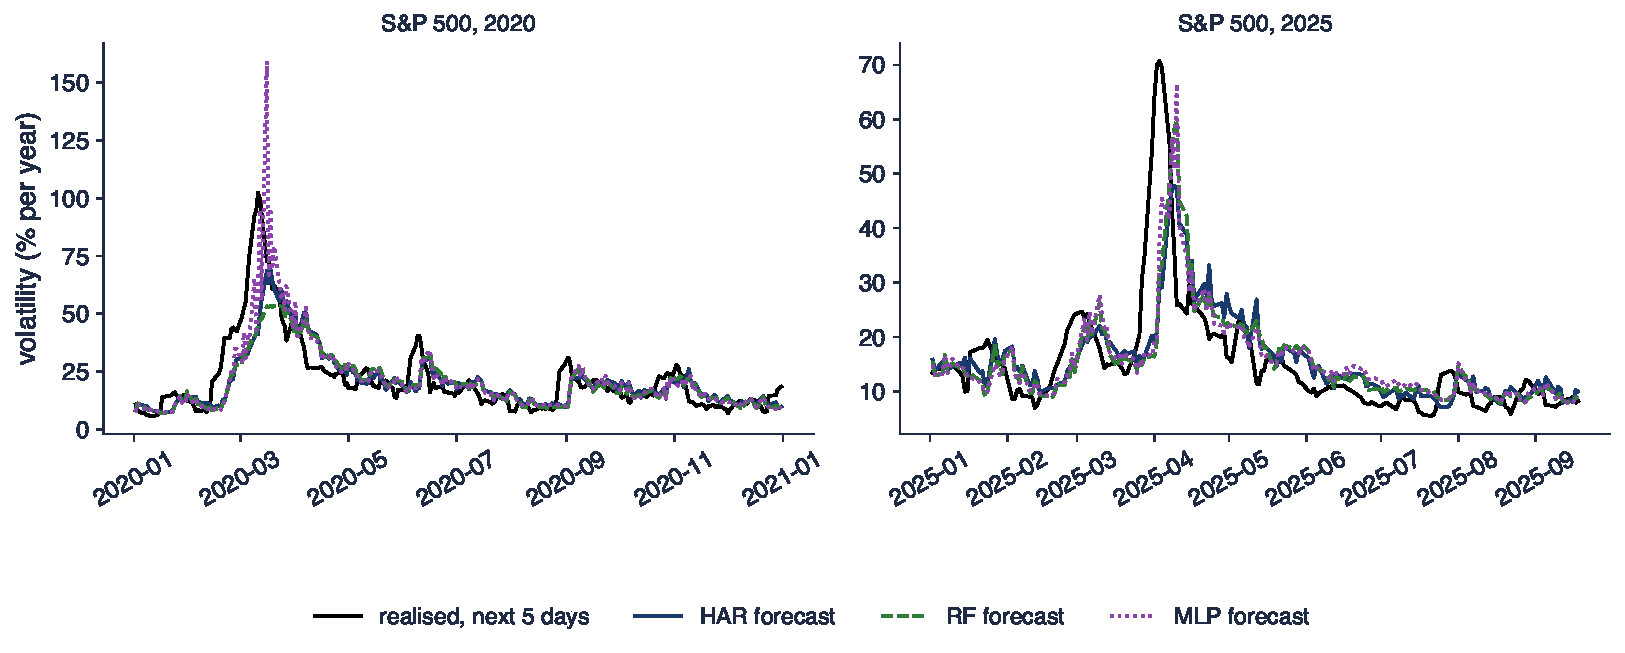
\includegraphics[width=0.97\textwidth,height=0.50\textheight,keepaspectratio]{sfm_ch13_rv_forecasts.pdf}
\end{center}
\vspace{-0.25cm}
\begin{itemize}
    \item S\&P 500: volatilitatea realizată anualizată din următoarele 5 zile, $\sqrt{252\,\mathrm{RV}_t}$, și prognozele HAR, random forest și MLP făcute la închiderea zilei $t$
    \item Interpretare: toate modelele reacționează abia după primul șoc (martie 2020, aprilie 2025); random forest este limitat de cele mai mari valori văzute în antrenare, iar MLP poate depăși ținta
\end{itemize}
\sfmquantlet{Ch_13}{SFM_ch13_volatility_forecast}
\end{frame}

\begin{frame}{Importanța variabilelor: permutare și valori Shapley}
\itemsize{\small}
\begin{itemize}
    \item \textbf{Importanța prin permutare}: amestecăm o variabilă în datele de test și măsurăm cu cît crește MSE de test
    \begin{itemize}
        \item creștere mare: modelul se bazează pe variabilă; variabilele corelate își împart (și își ascund) importanța
    \end{itemize}
    \item \textbf{Valorile Shapley} (teoria jocurilor): $\hat f(x) = \phi_0 + \sum_j \phi_j(x)$, $\phi_j$ este contribuția echitabilă a variabilei $j$ la prognoză
    \begin{itemize}
        \item $\phi_0$: prognoza medie; $\phi_j(x) > 0$: variabila $j$ ridică această prognoză peste medie, $\phi_j(x) < 0$: o coboară
        \item $\phi_j$ este media modificării lui $\hat f$ cînd $j$ se adaugă la fiecare submulțime a celorlalte variabile
        \item SHAP (Shapley additive explanations) \refLL: versiuni rapide pentru arbori; pentru un model liniar $\phi_j = \beta_j(x_j - \bar x_j)$
    \end{itemize}
    \item Ambele descriu modelul, nu economia: importanța nu înseamnă cauzalitate
\end{itemize}
\end{frame}

\begin{frame}{Variabilele folosite de random forest}
\itemsize{\footnotesize}
\begin{center}
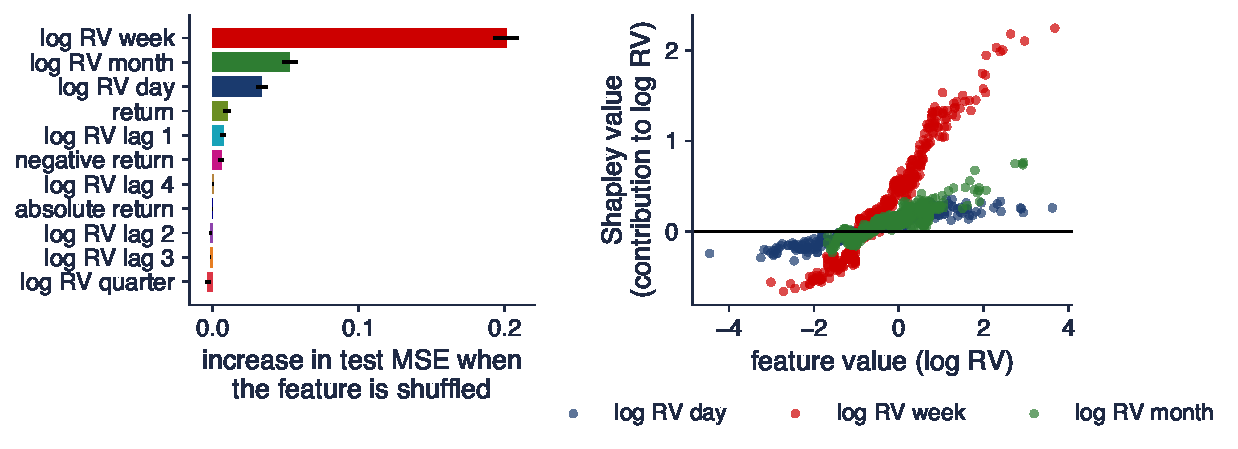
\includegraphics[width=0.97\textwidth,height=0.48\textheight,keepaspectratio]{sfm_ch13_importance.pdf}
\end{center}
\vspace{-0.25cm}
\begin{itemize}
    \item Stînga: random forest pe 11 variabile, antrenat pînă în 2019, testat în 2020--2026 (1\,682 de zile): amestecarea varianței săptămînale crește MSE cu $0{,}201$, a celei lunare cu $0{,}053$, a celei zilnice cu $0{,}034$
    \item Dreapta: valorile Shapley exacte ale unui random forest pe cele 3 variabile HAR; media $|\phi|$: săptămîna $0{,}52$, luna $0{,}13$, ziua $0{,}13$; efectul este neliniar și crește cu nivelul volatilității
\end{itemize}
\sfmquantlet{Ch_13}{SFM_ch13_volatility_forecast}
\end{frame}

\begin{frame}{Recapitulare: prognoza volatilității realizate}
\itemsize{\small}
\begin{itemize}
    \item HAR este un reper puternic; modelele penalizate și rețelele adaugă cîteva procente la S\&P 500, nimic la Bitcoin
    \item Evaluăm prin $R^2$ în afara eșantionului, QLIKE și Diebold--Mariano, într-un design walk-forward
    \item Varianța săptămînală conține cea mai mare parte din informație; măsurile de importanță descriu modelul, nu cauzele
\end{itemize}
\end{frame}


%=============================================================================
\section{Aplicație: semnul randamentului de mîine}
%=============================================================================

\begin{frame}{O problemă de clasificare}
\itemsize{\small}
\begin{itemize}
    \item Ținta: $y_t = \mathbf{1}\{r_{t+1} > 0\}$; variabilele la închiderea zilei $t$: ultimele 5 randamente, sumele pe 5, 21 și 63 de zile, volatilitatea pe 21 și 63 de zile
    \begin{itemize}
        \item $\mathbf{1}\{\cdot\}$: indicatorul, egal cu 1 dacă afirmația este adevărată și cu 0 în caz contrar; $y_t = 1$: randamentul de mîine este pozitiv
        \item modele: logit (\sfmchlink{https://danpele.github.io/SFM/RO/Cursuri/capitol12_modele_scoring.pdf}{Capitolul 12}), clasificatori random forest și gradient boosting; walk-forward, reestimare anuală
        \item S\&P 500 și BET din 2008, Bitcoin din 2018
    \end{itemize}
    \item Indicatori (definiți în \sfmchlink{https://danpele.github.io/SFM/RO/Cursuri/capitol12_modele_scoring.pdf}{Capitolul 12})
    \begin{itemize}
        \item acuratețea: ponderea zilelor cu semnul corect; AUC (aria de sub curba ROC): 0,5 înseamnă nicio capacitate de ordonare
    \end{itemize}
    \item Motivul unor așteptări modeste: eficiența în formă slabă (\sfmchlink{https://danpele.github.io/SFM/RO/Cursuri/capitol7_piete_eficiente_mers_aleator_vr.pdf}{Capitolul 7})
    \begin{itemize}
        \item orice tipar sigur din randamentele trecute ar dispărea prin tranzacționare
    \end{itemize}
\end{itemize}
\end{frame}

\begin{frame}{Reperul corect}
\itemsize{\small}
\begin{itemize}
    \item \textbf{Reperul clasei majoritare}: prognozăm mereu clasa mai frecventă din eșantionul de antrenare (aici: „creștere”)
    \begin{itemize}
        \item S\&P 500 din 2008: 54{,}4\% din zile sînt în creștere, deci „mereu creștere” are dreptate în 54{,}4\% din zile
        \item o acuratețe de 53\% pare o abilitate; față de acest reper este o pierdere
    \end{itemize}
    \item Testul față de reper: $z = (\widehat{\mathrm{acc}} - \mathrm{acc}_0)/\sqrt{\mathrm{acc}_0(1 - \mathrm{acc}_0)/n}$
    \begin{itemize}
        \item $\widehat{\mathrm{acc}}$: acuratețea modelului; $\mathrm{acc}_0$: acuratețea reperului; $n$: zilele de test; $z \approx N(0,1)$ dacă modelul nu are un avantaj real
        \item S\&P 500, $n = 4\,705$: eroarea standard 0{,}73 puncte; o bandă de 95\% de $\pm$1{,}4 puncte în jurul reperului
        \item random forest: 53{,}1\%, $z = -1{,}79$ (p 0{,}074); boosting: 52{,}1\%, $z = -3{,}19$ (p 0{,}001)
    \end{itemize}
    \item Pentru randamente, reperul corespunzător este prognoza zero sau media istorică \refWG
\end{itemize}
\end{frame}

\begin{frame}{Acuratețea față de reper}
\itemsize{\footnotesize}
\begin{center}
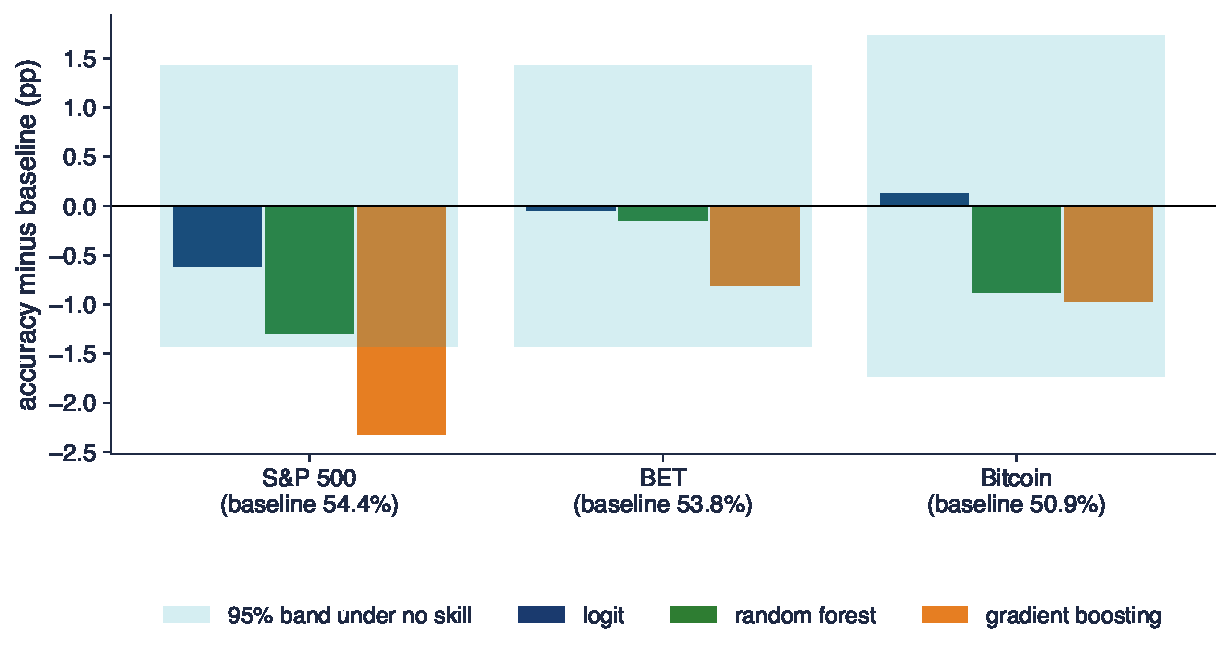
\includegraphics[width=0.97\textwidth,height=0.48\textheight,keepaspectratio]{sfm_ch13_sign.pdf}
\end{center}
\vspace{-0.25cm}
\begin{itemize}
    \item Acuratețea minus acuratețea reperului (puncte procentuale); banda: $\pm 1{,}96$ erori standard în jurul lui zero
    \item AUC pentru logit și pentru random forest: S\&P 500 0{,}511 și 0{,}507, BET 0{,}533 și 0{,}533, Bitcoin 0{,}515 și 0{,}519; logit prognozează „creștere” în 86\% din zilele S\&P 500
\end{itemize}
\sfmquantlet{Ch_13}{SFM_ch13_sign_prediction}
\end{frame}

\begin{frame}{Interpretare: eșecul obișnuit al prognozei semnului}
\itemsize{\small}
\begin{itemize}
    \item Pe nicio piață, niciun model nu este semnificativ superior regulii „mereu creștere”; modelele flexibile sînt mai slabe decît logit
    \begin{itemize}
        \item S\&P 500: logit $-0{,}6$, random forest $-1{,}3$, boosting $-2{,}3$ puncte; Bitcoin: logit $+0{,}1$, random forest $-0{,}9$
    \end{itemize}
    \item Raportul semnal--zgomot al randamentelor zilnice este foarte mic
    \begin{itemize}
        \item modelele flexibile găsesc tipare în zgomotul anilor de antrenare (secțiunea 2); logit este aproape de reper deoarece aproape nu se mișcă
    \end{itemize}
    \item Chiar și un avantaj real de un punct procentual ar rămîne rareori profitabil după costurile de tranzacționare: o strategie zilnică bazată pe semn tranzacționează foarte des
    \begin{itemize}
        \item cîștigurile aduse de machine learning în prognoza randamentelor provin din secțiuni transversale mari, pe orizonturi lunare, nu dintr-un singur indice pentru ziua următoare (secțiunea 11)
    \end{itemize}
\end{itemize}
\end{frame}

\begin{frame}{Recapitulare: semnul randamentului de mîine}
\itemsize{\small}
\begin{itemize}
    \item Comparați întotdeauna acuratețea cu reperul clasei majoritare și testați diferența
    \item Pe S\&P 500, BET și Bitcoin niciun model nu este semnificativ superior regulii „mereu creștere”
    \item Eficiența în formă slabă (\sfmchlink{https://danpele.github.io/SFM/RO/Cursuri/capitol7_piete_eficiente_mers_aleator_vr.pdf}{Capitolul 7}) prezice acest rezultat
\end{itemize}
\end{frame}


%=============================================================================
\section{Aplicație: VaR 1\% prin metode cuantilice}
%=============================================================================

\begin{frame}{Regresia cuantilică (1/2)}
\itemsize{\small}
\begin{itemize}
    \item \refKB: estimăm cuantila condiționată de ordin $\alpha$, $q_\alpha(x) = x^\top\beta_\alpha$, minimizînd \textbf{pierderea cuantilică} (pinball loss)
    \begin{itemize}
        \item $q_\alpha(x)$: nivelul sub care $y$ se află cu probabilitatea $\alpha$, condiționat de $x$; $\beta_\alpha$: coeficienți specifici nivelului $\alpha$
    \end{itemize}
    \item Pierderea pentru o eroare $u = y - q$: \[ \rho_\alpha(u) = u\,(\alpha - \mathbf{1}\{u < 0\}) \]
    \begin{itemize}
        \item sub cuantilă ($u < 0$) eroarea costă $(1 - \alpha)|u|$, deasupra ei $\alpha|u|$
        \item cu $\alpha = 0{,}01$, minimul se atinge cînd aproximativ 1\% din observații se află sub $q$
    \end{itemize}
\end{itemize}
\end{frame}

\begin{frame}{Regresia cuantilică (2/2)}
\itemsize{\small}
\begin{itemize}
    \item Cu $\alpha = 0{,}01$ și $q = -\mathrm{VaR}$: pierderea cuantilică medie din \sfmchlink{https://danpele.github.io/SFM/RO/Cursuri/capitol10_var_es_backtesting.pdf}{Capitolul 10}
    \begin{itemize}
        \item $(\alpha - I_t)(r_t + \mathrm{VaR}_t)$, cu $I_t = 1$ dacă $r_t < -\mathrm{VaR}_t$ (o depășire) și 0 în rest
    \end{itemize}
    \item VaR 1\% pentru ziua $t + 1$: $\widehat{\mathrm{VaR}}_t = -\hat q_{0{,}01}(x_t)$, cu $x_t$ = volatilitatea zilnică, săptămînală și lunară (rădăcinile variabilei proxy) și $r_t$
    \begin{itemize}
        \item nu presupunem nicio distribuție: datele aleg cum se transformă volatilitatea în coadă; CAViaR \refCAViaR{} este o versiune dinamică
    \end{itemize}
    \item \textbf{Quantile gradient boosting}: aceeași pierdere, cu arbori în boosting (secțiunea 5)
    \begin{itemize}
        \item flexibil, dar la 1\% fiecare frunză vede puține observații din coadă: varianță mare
    \end{itemize}
\end{itemize}
\end{frame}

\begin{frame}{Backtesting pentru VaR 1\%: metode cuantilice, HS și GARCH-t}
\itemsize{\footnotesize}
\begin{center}
\scriptsize
\begin{tabular}{llrrrrrr}
\toprule
& Metoda & $x$ & rata (\%) & p Kupiec & p ind. & pierdere $\times 100$ & VaR mediu \\
\midrule
S\&P 500 & QR & 28 & $0{,}81$ & 0{,}252 & 0{,}020 & $3{,}38$ & $2{,}70$ \\
 & QGB & 42 & $1{,}22$ & 0{,}213 & 0{,}015 & $3{,}51$ & $2{,}46$ \\
 & HS & 46 & $1{,}33$ & 0{,}061 & $<$\,0{,}001 & $4{,}78$ & $2{,}97$ \\
 & GARCH-t & 52 & $1{,}51$ & 0{,}005 & 0{,}008 & $3{,}50$ & $2{,}42$ \\
\midrule
Bitcoin & QR & 23 & $0{,}72$ & 0{,}098 & 0{,}563 & $13{,}03$ & $10{,}46$ \\
 & QGB & 47 & $1{,}48$ & 0{,}012 & 0{,}235 & $13{,}19$ & $8{,}86$ \\
 & HS & 32 & $1{,}01$ & 0{,}974 & 0{,}332 & $13{,}01$ & $9{,}30$ \\
 & GARCH-t & 41 & $1{,}29$ & 0{,}117 & 0{,}558 & $13{,}15$ & $8{,}52$ \\
\bottomrule
\end{tabular}
\end{center}
\begin{itemize}
    \item QR: regresie cuantilică liniară; QGB: quantile gradient boosting; HS: simulare istorică pe 500 de zile; GARCH-t: reestimat în fiecare ianuarie (\sfmchlink{https://danpele.github.io/SFM/RO/Cursuri/capitol10_var_es_backtesting.pdf}{Capitolul 10}); p ind.: testul de independență Christoffersen
    \item S\&P 500 (3\,448 de zile de la 2 ianuarie 2013): QR are rata corectă (0{,}81\%) și cea mai mică pierdere, dar depășirile lui nu sînt complet independente (p ind.\ 0{,}020); GARCH-t este depășit prea des (1{,}51\%)
    \item Bitcoin (3\,182 de zile): HS are cea mai bună rată (1{,}01\%); QGB este respins (1{,}48\%, p 0{,}012)
\end{itemize}\sfmquantlet{Ch_13}{SFM_ch13_quantile_var}
\end{frame}

\begin{frame}{Prognozele VaR 1\% în 2020 și 2025}
\itemsize{\footnotesize}
\begin{center}
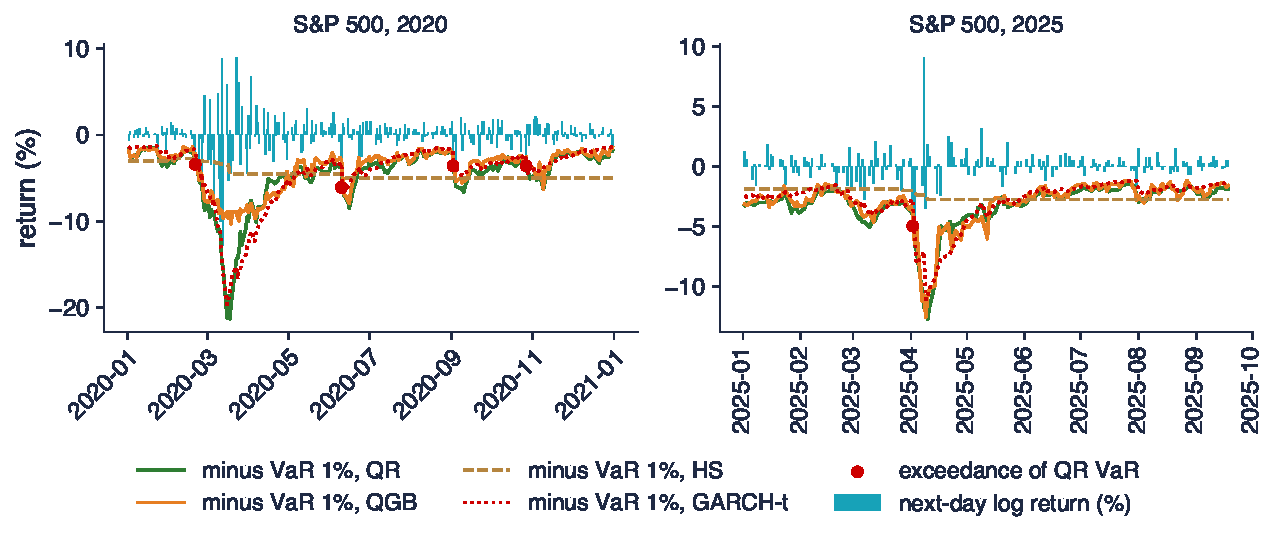
\includegraphics[width=0.97\textwidth,height=0.48\textheight,keepaspectratio]{sfm_ch13_qvar.pdf}
\end{center}
\vspace{-0.25cm}
\begin{itemize}
    \item S\&P 500: randamentele zilei următoare și minus VaR 1\% pentru cele patru metode; punctele: depășirile VaR obținut prin regresie cuantilică
    \item Interpretare: QR și GARCH-t urmează volatilitatea; HS reacționează lent; în 2020, HS a fost depășit de 10 ori, QR de 4 ori, iar depășirile HS apar grupat (p ind.\ $<$\,0{,}001)
\end{itemize}
\sfmquantlet{Ch_13}{SFM_ch13_quantile_var}
\end{frame}

\begin{frame}{Recapitulare: VaR 1\% prin metode cuantilice}
\itemsize{\small}
\begin{itemize}
    \item Regresia cuantilică minimizează pierderea cuantilică: VaR fără o ipoteză despre distribuție
    \item Un model cuantilic liniar pe variabile de volatilitate trece testul Kupiec pentru S\&P 500
    \item Modelele cuantilice flexibile la 1\% au nevoie de mult mai multe date din coadă decît avem
\end{itemize}
\end{frame}


%=============================================================================
\section{Data snooping și raportul Sharpe deflatat}
%=============================================================================

\begin{frame}{Cea mai bună dintre $N$ strategii (1/2)}
\itemsize{\small}
\begin{itemize}
    \item \textbf{Data snooping}: încercarea multor modele sau reguli pe aceleași date și raportarea celei mai bune \refWhite
    \begin{itemize}
        \item cu suficiente încercări, o regulă fără nicio abilitate pare excelentă în eșantion
        \item sute de predictori ai randamentelor publicați nu ar trece de o corecție pentru testare multiplă \refHLZ
    \end{itemize}
    \item Raportul Sharpe anual al unei strategii fără abilitate pe $Y$ ani este aproximativ $N(0, 1/Y)$
    \begin{itemize}
        \item raportul Sharpe: randamentul mediu în exces împărțit la abaterea lui standard (\sfmchlink{https://danpele.github.io/SFM/RO/Cursuri/capitol1_date_randamente_indicatori.pdf}{Capitolul 1}); $Y$: numărul de ani de date
        \item media 0: nicio abilitate; varianța $1/Y$: eroarea de estimare, care scade odată cu lungimea eșantionului
    \end{itemize}
\end{itemize}
\end{frame}

\begin{frame}{Cea mai bună dintre $N$ strategii (2/2)}
\itemsize{\small}
\begin{itemize}
    \item Maximul așteptat al celor $N$ încercări independente, fără abilitate \refBLdP{} \[ \mathrm{E}[\max] \approx \sigma\Big[(1 - \gamma)\,\Phi^{-1}\big(1 - \tfrac1N\big) + \gamma\,\Phi^{-1}\big(1 - \tfrac{1}{Ne}\big)\Big] \]
    \begin{itemize}
        \item $\sigma$: abaterea standard a rapoartelor Sharpe între încercări ($1/\sqrt{Y}$ mai sus); $N$: numărul de încercări
        \item $\Phi^{-1}$: funcția cuantilă a distribuției Normale standard; $e \approx 2{,}718$; $\gamma = 0{,}5772$: constanta Euler--Mascheroni
    \end{itemize}
    \item Exemplu: 10 ani, $\sigma = 1/\sqrt{10} = 0{,}316$, $N = 100$
    \begin{itemize}
        \item $0{,}316\,[(1 - \gamma)\,2{,}326 + \gamma\,2{,}680] = 0{,}80$: un asemenea raport Sharpe apare, în medie, doar prin noroc
        \item simulare: cea mai bună dintre 10, 100 și 1000 de strategii fără abilitate are un raport Sharpe mediu de $0{,}48$; $0{,}79$; $1{,}02$
    \end{itemize}
\end{itemize}
\end{frame}

\begin{frame}{Distorsiunea de selecție în practică}
\itemsize{\footnotesize}
\begin{center}
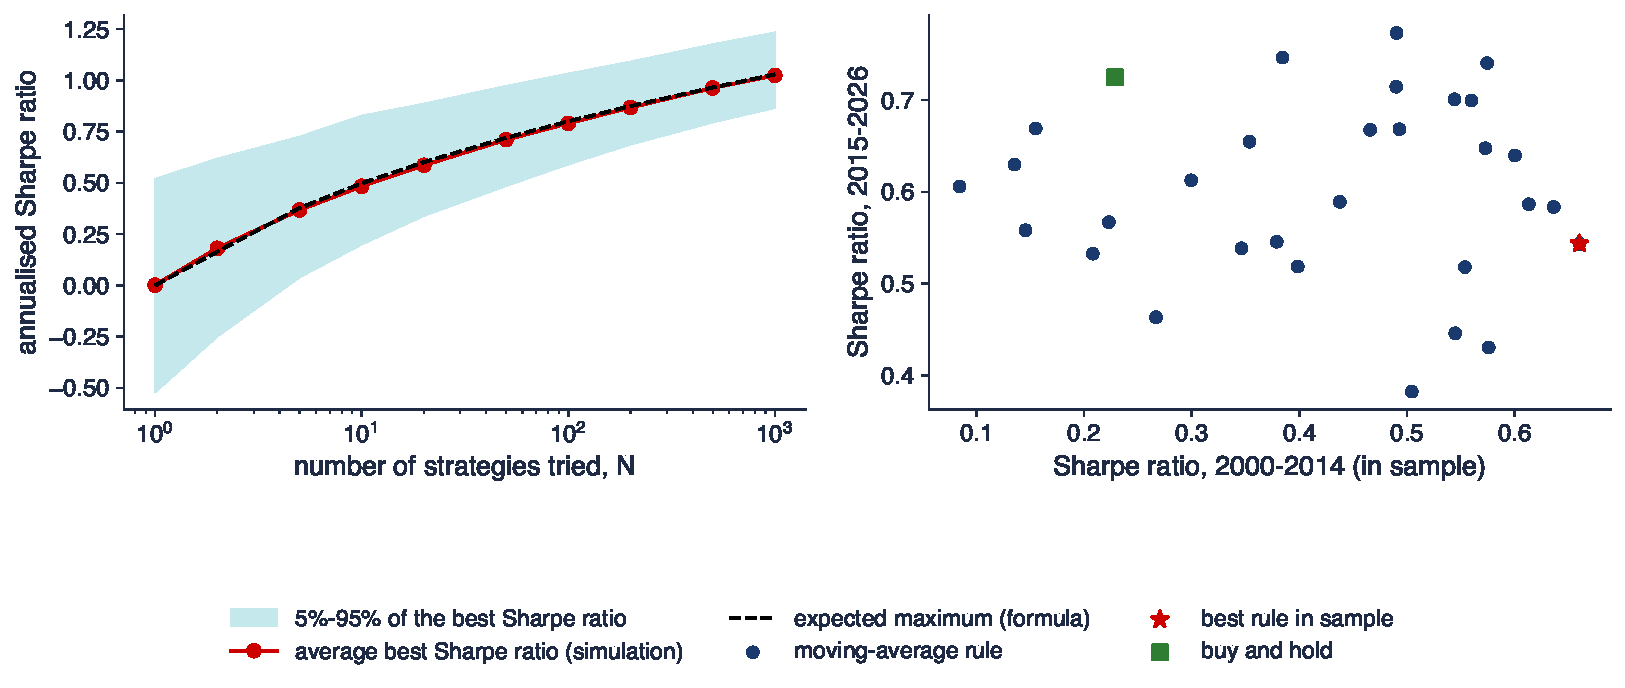
\includegraphics[width=0.97\textwidth,height=0.48\textheight,keepaspectratio]{sfm_ch13_snooping.pdf}
\end{center}
\vspace{-0.25cm}
\begin{itemize}
    \item Stînga: cel mai bun raport Sharpe anual dintre $N$ strategii fără abilitate (10 ani); dreapta: 30 de reguli cu medii mobile pe S\&P 500 (investit sau numerar), 2000--2014 față de 2015--2026
    \item Interpretare: cea mai bună regulă în eșantion (MA 50/200, Sharpe $0{,}66$) obține apoi $0{,}54$, locul 22 din 30, sub buy and hold ($0{,}72$); rapoartele Sharpe din eșantion și din afara lui au corelația $0{,}04$
\end{itemize}
\sfmquantlet{Ch_13}{SFM_ch13_data_snooping}
\end{frame}

\begin{frame}{Raportul Sharpe deflatat (1/2)}
\itemsize{\small}
\begin{itemize}
    \item \refBLdP: probabilitatea ca adevăratul raport Sharpe să depășească ceea ce ar arăta din noroc cea mai bună dintre $N$ încercări \[ \mathrm{DSR} = \Phi\Big(\dfrac{(\widehat{SR} - SR_0)\sqrt{T - 1}}{\sqrt{1 - \hat\gamma_3\widehat{SR} + \frac{\hat\gamma_4 - 1}{4}\widehat{SR}^2}}\Big) \]
    \item Notațiile
    \begin{itemize}
        \item $\widehat{SR}$: raportul Sharpe zilnic al strategiei alese; $T$: numărul de zile
        \item $SR_0$: maximul așteptat al celor $N$ încercări fără abilitate (mai sus), cu $\sigma$ = abaterea standard a celor $N$ rapoarte Sharpe încercate
        \item $\hat\gamma_3$: asimetria, $\hat\gamma_4$: boltirea randamentelor zilnice (3 pentru distribuția Normală); $\Phi$: funcția de repartiție Normală standard
    \end{itemize}
    \item Interpretarea
    \begin{itemize}
        \item DSR este o probabilitate în $(0, 1)$; peste 0,95: raportul Sharpe este semnificativ după corecția pentru $N$ încercări
        \item asimetria negativă și cozile groase măresc numitorul și reduc DSR
    \end{itemize}
\end{itemize}
\end{frame}

\begin{frame}{Raportul Sharpe deflatat (2/2)}
\itemsize{\small}
\begin{itemize}
    \item \textbf{Pas cu pas}: cea mai bună regulă MA, $N = 30$, $T = 3\,769$ de zile
    \begin{itemize}
        \item $\widehat{SR} = 0{,}0416$ pe zi ($\times\sqrt{252} = 0{,}66$); $\hat\gamma_3 = -0{,}44$, $\hat\gamma_4 = 12{,}0$
        \item $SR_0 = 0{,}0105\,[(1 - \gamma)\,1{,}834 + \gamma\,2{,}249] = 0{,}0219$ (anual $0{,}35$)
        \item $z = 1{,}20$, DSR $= 0{,}88$; fără corecția pentru $N$ (PSR, $SR_0 = 0$): $0{,}994$
    \end{itemize}
    \item Interpretare: luată singură, regula pare semnificativă; după 30 de încercări nu mai este (DSR sub 0,95), așa cum confirmă și rezultatele ulterioare
\end{itemize}
\end{frame}

\begin{frame}{Recapitulare: data snooping}
\itemsize{\small}
\begin{itemize}
    \item Cel mai bun rezultat dintre multe încercări este deplasat în sus; deplasarea crește proporțional cu $\sqrt{2\ln N}$
    \item Raportați numărul de încercări și deflatați raportul Sharpe
    \item Un eșantion de test final folosit o singură dată este protecția cea mai simplă
\end{itemize}
\end{frame}


%=============================================================================
\section{Studiu de caz: Gu, Kelly și Xiu (2020)}
%=============================================================================

\begin{frame}{Empirical Asset Pricing via Machine Learning}
\itemsize{\footnotesize}
\begin{columns}[T]
\begin{column}{0.60\textwidth}
\begin{itemize}
    \item \refGKX: care metode prezic cel mai bine randamentul lunar al acțiunilor americane individuale?
    \begin{itemize}
        \item aproape 30\,000 de acțiuni, 1957--2016; 94 de caracteristici ale firmelor, în interacțiune cu 8 variabile macroeconomice, plus 74 de variabile indicatoare de industrie: 920 de variabile
    \end{itemize}
    \item Schema de estimare: 18 ani de antrenare (1957--1974), 12 de validare (1975--1986), 30 de test (1987--2016)
    \begin{itemize}
        \item reestimare o dată pe an; fereastra de antrenare crește, cea de validare avansează: o schemă walk-forward
        \item modele: OLS, regresii penalizate și cu reducerea dimensiunii, random forest, arbori în boosting, rețele cu 1--5 straturi ascunse
    \end{itemize}
\end{itemize}
\end{column}
\begin{column}{0.36\textwidth}
\centering

\includegraphics[height=0.36\textheight]{ch13_harper_center_2013.jpg}\\[1mm]
\imgcap{Charles M.\ Harper Center, Chicago Booth, unde au lucrat Gu și Xiu}
\imgcredit{https://commons.wikimedia.org/wiki/File:University_of_Chicago_July_2013_01_(Charles_M._Harper_Center).jpg}{Foto: Michael Barera (2013); CC BY-SA 4.0; Wikimedia Commons}
\end{column}
\end{columns}
\end{frame}

\begin{frame}{Evaluarea din lucrare}
\itemsize{\small}
\begin{itemize}
    \item $R^2_{OOS} = 1 - \sum_{(i,t)}(r_{i,t+1} - \hat r_{i,t+1})^2 / \sum_{(i,t)} r_{i,t+1}^2$: reperul este o prognoză \textbf{zero}, nu media istorică
    \begin{itemize}
        \item $r_{i,t+1}$: randamentul acțiunii $i$ în luna $t + 1$; $\hat r_{i,t+1}$: prognoza lui; sumele parcurg toate perechile acțiune--lună din perioada de test
        \item autorii arată că media istorică a unei acțiuni este atît de zgomotoasă încît este ușor de depășit: reperul zero este mai exigent
    \end{itemize}
    \item Teste Diebold--Mariano între toate perechile de modele, cu o corecție Bonferroni pentru cele 12 comparații (pragul de semnificație se împarte la numărul comparațiilor)
    \begin{itemize}
        \item același instrument ca în secțiunea 7, aplicat unui panel de acțiuni
    \end{itemize}
    \item Valoarea economică: în fiecare lună, sortăm acțiunile în decile după prognoză; cumpărăm decila de sus și vindem decila de jos
    \begin{itemize}
        \item portofolii ponderate cu valoarea de piață; raportul Sharpe, drawdown și rulajul (ponderea portofoliului tranzacționată lunar)
    \end{itemize}
\end{itemize}
\end{frame}

\begin{frame}{Rezultatele: $R^2$ mic, valoare economică mare}
\itemsize{\footnotesize}
\begin{center}
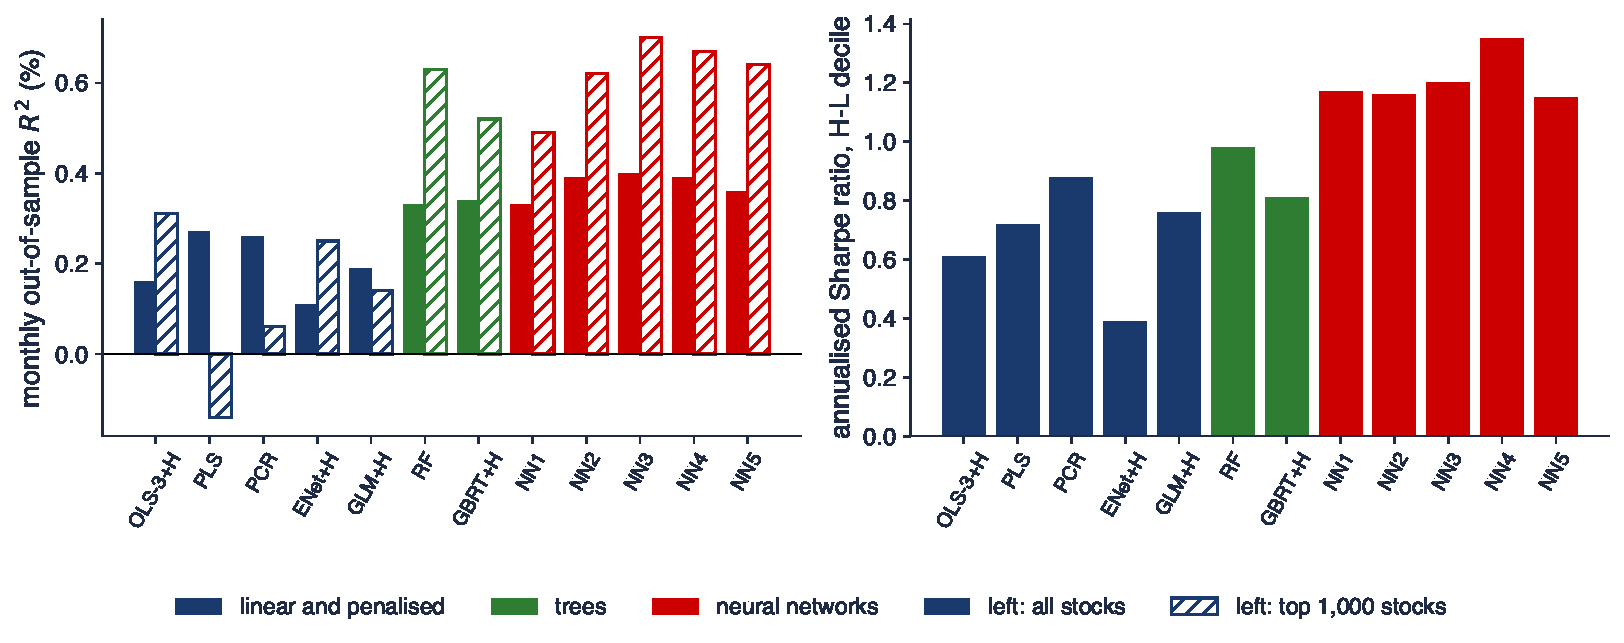
\includegraphics[width=0.97\textwidth,height=0.48\textheight,keepaspectratio]{sfm_ch13_gkx.pdf}
\end{center}
\vspace{-0.25cm}
\begin{itemize}
    \item Stînga: $R^2_{OOS}$ lunar (tabelul 1): OLS cu toate cele 920 de variabile $-3{,}46\%$; OLS-3 (mărime, valoare, momentum) $0{,}16\%$; random forest $0{,}33\%$; NN3 $0{,}40\%$ ($0{,}70\%$ pentru cele mai mari 1\,000 de acțiuni)
    \item Dreapta: raportul Sharpe anual al diferenței dintre decile, ponderată cu valoarea de piață (tabelul 7): OLS-3 $0{,}61$, random forest $0{,}98$, NN4 $1{,}35$
\end{itemize}
\sfmquantlet{Ch_13}{SFM_ch13_case_gkx}
\end{frame}

\begin{frame}{Interpretare și limite}
\itemsize{\small}
\begin{itemize}
    \item Rezultatele lucrării
    \begin{itemize}
        \item modelele neliniare (arbori, rețele) sînt superioare celor liniare deoarece surprind interacțiunile dintre caracteristici
        \item toate metodele sînt de acord asupra semnalelor principale: tendințele prețului (momentum, inversarea pe termen scurt), lichiditatea, volatilitatea
        \item rețelele puțin adînci sînt suficiente: 3--4 straturi dau rezultate mai bune decît 5; deep learning nu ajută la randamentele lunare
    \end{itemize}
    \item De reținut
    \begin{itemize}
        \item un $R^2_{OOS}$ sub 1\% pe lună este un rezultat important în acest context: comparați cu prognozele semnului din secțiunea 8
        \item portofoliile pe baza rețelelor își schimbă lunar peste 100\% din valoare: costurile de tranzacționare reduc cîștigurile
        \item dovezile provin dintr-o secțiune transversală de mii de acțiuni; ele spun puțin despre alegerea momentului pentru un singur indice
    \end{itemize}
\end{itemize}
\end{frame}


%=============================================================================
\section{AI pentru descoperire științifică}
%=============================================================================

\begin{frame}{O întrebare deschisă}
\itemsize{\small}
\begin{itemize}
    \item \textbf{Ajută prognozele de volatilitate prin machine learning la Bursa de Valori București, unde lichiditatea este redusă și datele intrazilnice sînt rare?}
    \begin{itemize}
        \item azi: la S\&P 500, lasso cîștigă $+7{,}1\%$ față de HAR; la Bitcoin niciun cîștig semnificativ ($+2{,}0\%$, p 0{,}520)
        \item BET nu are prețuri maxime și minime în datele noastre, deci variabila proxy trebuie construită din randamente la pătrat, mai zgomotoase
    \end{itemize}
    \item Întrebarea rămîne deschisă: tranzacționare rară, un calendar diferit de cel de la New York, puține crize în eșantion
    \item Lucrări înrudite, ca lectură suplimentară: \refPeleA{} (clasificarea statistică a activelor cripto); \refPeleB{} (cît de precise pot fi comparațiile de prognoze)
    \item Instrumentele AI pot accelera un astfel de studiu; nu înlocuiesc verificarea lui \refWang
\end{itemize}
\end{frame}

\begin{frame}{Contribuția posibilă a AI}
\itemsize{\small}
\begin{itemize}
    \item \textbf{Literatura}: o listă a studiilor despre HAR și machine learning pentru piețele emergente și de frontieră
    \item \textbf{Cod}: o primă versiune a comparației walk-forward dintre HAR, lasso și random forest pentru BET și trei acțiuni BVB
    \item \textbf{Robustețe}: alte variabile proxy (randamente absolute, randamente pe două zile), alte orizonturi (1, 5, 22 de zile), variabile S\&P 500 de la închiderea precedentă
    \item Exemplu de prompt
    \begin{itemize}
        \item \aiprompt{Write Python code that compares HAR, lasso and a random forest for the weekly log variance of the BET index (proxy: squared daily returns), with yearly walk-forward refits from 2012, purging the last 5 training rows, and reports the out-of-sample R2, QLIKE and Diebold-Mariano tests.}
    \end{itemize}
\end{itemize}
\end{frame}

\begin{frame}{Verificări necesare}
\itemsize{\small}
\begin{itemize}
    \item Ordinea temporală: fără partiții amestecate; variabilele folosesc doar date pînă la închiderea zilei $t$; ultimele ținte de antrenare nu ajung în perioada de test
    \item Scalarea și alegerea hiperparametrilor doar în fereastra de antrenare (standardizarea, $\lambda$, numărul de arbori)
    \item Calendarele: BVB se închide înaintea bursei din New York; variabilele S\&P 500 trebuie să provină de la închiderea precedentă din New York
    \item Un reper în fiecare tabel (HAR, clasa majoritară, simularea istorică) și un test al diferenței
    \item Numărul de modele încercate, raportat; referințele: fiecare lucrare citată trebuie să existe; verificați DOI-ul
\end{itemize}
\end{frame}

\begin{frame}{Idee de proiect}
\itemsize{\small}
\begin{itemize}
    \item \textbf{Întrebarea}: prognozează modelele de machine learning volatilitatea acțiunilor BVB mai bine decît HAR?
    \begin{itemize}
        \item date: BET, Banca Transilvania, OMV Petrom, BRD (EODHD); S\&P 500 și DAX ca variabile externe
    \end{itemize}
    \item Pași
    \begin{itemize}
        \item o variabilă proxy a varianței pentru fiecare acțiune (amplitudinea, unde există, altfel randamentele la pătrat), țintă săptămînală
        \item HAR, lasso, random forest și un MLP mic, walk-forward din 2014, reestimare anuală cu purging
        \item $R^2$ în afara eșantionului, QLIKE și Diebold--Mariano; valori Shapley pentru variabilele externe
    \end{itemize}
    \item Livrabil: un tabel, un grafic și un paragraf despre ce pot și ce nu pot arăta datele
    \item Declarați orice utilizare a instrumentelor AI și enumerați erorile acestora pe care le-ați corectat
\end{itemize}
\end{frame}


%=============================================================================
\section{Rezumat}
%=============================================================================

\begin{frame}{Idei de reținut}
\itemsize{\small}
\begin{itemize}
    \item Machine learning se judecă după eroarea pe date noi; compromisul deplasare--varianță stabilește cît de flexibil trebuie să fie un model
    \item Seriile de timp au nevoie de validare walk-forward cu purging; partițiile aleatoare pe ținte suprapuse simulează o predictibilitate falsă
    \item Ridge și lasso contractă coeficienții; random forest face media arborilor; boosting adaugă arbori; rețelele învață variabile neliniare
    \item Volatilitatea: HAR este greu de depășit, cîștigurile sînt de cîteva procente; semnul randamentelor: niciun cîștig față de „mereu creștere”
    \item VaR 1\%: regresia cuantilică liniară funcționează; modelelor cuantilice flexibile le lipsesc datele din coadă
    \item Raportați numărul de încercări și deflatați raportul Sharpe; comparați fiecare model cu un reper simplu
\end{itemize}
\end{frame}

\begin{frame}{Formule de reținut}
\itemsize{\small}
{\renewcommand{\arraystretch}{1.45}\begin{center}
\scriptsize
\begin{tabular}{ll}
\toprule
\textbf{Mărimea} & \textbf{Formula} \\
\midrule
Deplasare--varianță & $E[(y_0 - \hat f)^2] = (E\hat f - f)^2 + \mathrm{Var}(\hat f) + \sigma^2$ \\
Ridge & $(X^\top X + \lambda I)^{-1}X^\top y$; \ 1D: $S_{xy}/(S_{xx} + \lambda)$ \\
Lasso (1D) & $\mathrm{sign}(S_{xy})\max(|S_{xy}| - \lambda/2, 0)/S_{xx}$ \\
Random forest & $\mathrm{Var} = \rho\sigma^2 + (1 - \rho)\sigma^2/B$ \\
Boosting & $F_m = F_{m-1} + \nu h_m$ \\
MLP & $\hat y = c + \sum_k v_k g(b_k + w_k^\top x)$ \\
HAR & $y_t = \beta_0 + \beta_d\ln v_t + \beta_w\ln v_t^{(w)} + \beta_m\ln v_t^{(m)} + u_t$ \\
$R^2_{OOS}$ & $1 - \sum(y - \hat y)^2/\sum(y - \tilde y)^2$ \\
Pierderea cuantilică & $\rho_\alpha(u) = u(\alpha - \mathbf{1}\{u < 0\})$ \\
DSR & $\Phi\big((\widehat{SR} - SR_0)\sqrt{T - 1}/\sqrt{1 - \hat\gamma_3\widehat{SR} + (\hat\gamma_4 - 1)\widehat{SR}^2/4}\big)$ \\
\bottomrule
\end{tabular}
\end{center}
}
\end{frame}

\begin{frame}{Autoevaluare}
\itemsize{\small}
\begin{itemize}
    \item \textbf{Întrebare}: un model are un $R^2$ de antrenare de 80\% și un $R^2$ în afara eșantionului de $-5\%$. Ce s-a întîmplat?
    \begin{itemize}
        \item \textbf{Răspuns}: overfitting: modelul a învățat zgomotul eșantionului de antrenare și pierde în fața reperului pe date noi
    \end{itemize}
    \item \textbf{Întrebare}: de ce este greșit K-fold aleator pentru o țintă de tip randament pe 21 de zile?
    \begin{itemize}
        \item \textbf{Răspuns}: țintele vecine se suprapun, deci răspunsurile de test ajung în antrenare; folosiți walk-forward cu purging
    \end{itemize}
    \item \textbf{Întrebare}: un clasificator are dreptate în 53\% din zile, iar piața a crescut în 54\% dintre ele. Este util?
    \begin{itemize}
        \item \textbf{Răspuns}: nu: „mereu creștere” are dreptate în 54\% din zile
    \end{itemize}
    \item Urmează: \sfmchlink{https://danpele.github.io/SFM/RO/Cursuri/capitol14_active_cripto.pdf}{Capitolul 14}, activele cripto
\end{itemize}
\end{frame}


%=============================================================================
\section{Bibliografie}
%=============================================================================

\begin{frame}{Bibliografie (1/3)}
\itemsize{\tiny}
\begin{itemize}
    \item Bailey, D.H., López de Prado, M. (2014). \href{https://doi.org/10.3905/jpm.2014.40.5.094}{The deflated Sharpe ratio: correcting for selection bias, backtest overfitting, and non-normality}. \textit{Journal of Portfolio Management}, 40(5), 94--107.
    \item Bergmeir, C., Hyndman, R.J., Koo, B. (2018). \href{https://doi.org/10.1016/j.csda.2017.11.003}{A note on the validity of cross-validation for evaluating autoregressive time series prediction}. \textit{Computational Statistics \& Data Analysis}, 120, 70--83.
    \item Breiman, L. (2001a). \href{https://doi.org/10.1214/ss/1009213726}{Statistical modeling: the two cultures}. \textit{Statistical Science}, 16(3), 199--231.
    \item Breiman, L. (2001b). \href{https://doi.org/10.1023/A:1010933404324}{Random forests}. \textit{Machine Learning}, 45(1), 5--32.
    \item Campbell, J.Y., Thompson, S.B. (2008). \href{https://doi.org/10.1093/rfs/hhm055}{Predicting excess stock returns out of sample: can anything beat the historical average?} \textit{Review of Financial Studies}, 21(4), 1509--1531.
    \item Christensen, K., Siggaard, M., Veliyev, B. (2023). \href{https://doi.org/10.1093/jjfinec/nbac020}{A machine learning approach to volatility forecasting}. \textit{Journal of Financial Econometrics}, 21(5), 1680--1727.
    \item Christoffersen, P.F. (1998). \href{https://doi.org/10.2307/2527341}{Evaluating interval forecasts}. \textit{International Economic Review}, 39(4), 841--862.
    \item Corsi, F. (2009). \href{https://doi.org/10.1093/jjfinec/nbp001}{A simple approximate long-memory model of realized volatility}. \textit{Journal of Financial Econometrics}, 7(2), 174--196.
    \item Diebold, F.X., Mariano, R.S. (1995). \href{https://doi.org/10.1080/07350015.1995.10524599}{Comparing predictive accuracy}. \textit{Journal of Business \& Economic Statistics}, 13(3), 253--263.
    \item Engle, R.F. (1982). \href{https://doi.org/10.2307/1912773}{Autoregressive conditional heteroscedasticity with estimates of the variance of United Kingdom inflation}. \textit{Econometrica}, 50(4), 987--1007.
    \item Engle, R.F., Manganelli, S. (2004). \href{https://doi.org/10.1198/073500104000000370}{CAViaR: conditional autoregressive value at risk by regression quantiles}. \textit{Journal of Business \& Economic Statistics}, 22(4), 367--381.
    \item Franke, J., Härdle, W.K., Hafner, C.M. (2019). \href{https://doi.org/10.1007/978-3-030-13751-9}{\textit{Statistics of Financial Markets: An Introduction}}, 5th ed. Springer.
    \item Friedman, J.H. (2001). \href{https://doi.org/10.1214/aos/1013203451}{Greedy function approximation: a gradient boosting machine}. \textit{Annals of Statistics}, 29(5), 1189--1232.
    \item Garman, M.B., Klass, M.J. (1980). \href{https://doi.org/10.1086/296072}{On the estimation of security price volatilities from historical data}. \textit{Journal of Business}, 53(1), 67--78.
    \item Gu, S., Kelly, B., Xiu, D. (2020). \href{https://doi.org/10.1093/rfs/hhaa009}{Empirical asset pricing via machine learning}. \textit{Review of Financial Studies}, 33(5), 2223--2273.
    \item Harvey, C.R., Liu, Y., Zhu, H. (2016). \href{https://doi.org/10.1093/rfs/hhv059}{\ldots and the cross-section of expected returns}. \textit{Review of Financial Studies}, 29(1), 5--68.
\end{itemize}
\end{frame}

\begin{frame}{Bibliografie (2/3)}
\itemsize{\tiny}
\begin{itemize}
    \item Hastie, T., Tibshirani, R., Friedman, J. (2009). \href{https://doi.org/10.1007/978-0-387-84858-7}{\textit{The Elements of Statistical Learning}}, 2nd ed. Springer.
    \item Hoerl, A.E., Kennard, R.W. (1970). \href{https://doi.org/10.1080/00401706.1970.10488634}{Ridge regression: biased estimation for nonorthogonal problems}. \textit{Technometrics}, 12(1), 55--67.
    \item Hornik, K., Stinchcombe, M., White, H. (1989). \href{https://doi.org/10.1016/0893-6080(89)90020-8}{Multilayer feedforward networks are universal approximators}. \textit{Neural Networks}, 2(5), 359--366.
    \item James, G., Witten, D., Hastie, T., Tibshirani, R., Taylor, J. (2023). \href{https://doi.org/10.1007/978-3-031-38747-0}{\textit{An Introduction to Statistical Learning with Applications in Python}}. Springer.
    \item Kelly, B., Xiu, D. (2023). \href{https://doi.org/10.1561/0500000064}{Financial machine learning}. \textit{Foundations and Trends in Finance}, 13(3--4), 205--363.
    \item Koenker, R., Bassett, G. (1978). \href{https://doi.org/10.2307/1913643}{Regression quantiles}. \textit{Econometrica}, 46(1), 33--50.
    \item Kupiec, P.H. (1995). \href{https://doi.org/10.3905/jod.1995.407942}{Techniques for verifying the accuracy of risk measurement models}. \textit{Journal of Derivatives}, 3(2), 73--84.
    \item Lundberg, S.M., Lee, S.-I. (2017). \href{https://proceedings.neurips.cc/paper/2017/hash/8a20a8621978632d76c43dfd28b67767-Abstract.html}{A unified approach to interpreting model predictions}. \textit{Advances in Neural Information Processing Systems}, 30.
    \item López de Prado, M. (2018). \href{https://www.wiley.com/en-us/Advances+in+Financial+Machine+Learning-p-9781119482086}{\textit{Advances in Financial Machine Learning}}. Wiley.
    \item Patton, A.J. (2011). \href{https://doi.org/10.1016/j.jeconom.2010.03.034}{Volatility forecast comparison using imperfect volatility proxies}. \textit{Journal of Econometrics}, 160(1), 246--256.
    \item Pele, D.T., Mazurencu-Marinescu-Pele, M. (2026). \href{https://doi.org/10.3390/math14132316}{Finite-sample precision limits for expected shortfall forecast comparisons}. \textit{Mathematics}, 14(13), 2316.
    \item Pele, D.T., Wesselhöfft, N., Härdle, W.K., Kolossiatis, M., Yatracos, Y.G. (2023). \href{https://doi.org/10.1080/1351847X.2021.1960403}{Are cryptos becoming alternative assets?} \textit{European Journal of Finance}, 29(10), 1064--1105.
    \item Rosenblatt, F. (1958). \href{https://doi.org/10.1037/h0042519}{The perceptron: a probabilistic model for information storage and organization in the brain}. \textit{Psychological Review}, 65(6), 386--408.
    \item Rumelhart, D.E., Hinton, G.E., Williams, R.J. (1986). \href{https://doi.org/10.1038/323533a0}{Learning representations by back-propagating errors}. \textit{Nature}, 323, 533--536.
    \item Tibshirani, R. (1996). \href{https://doi.org/10.1111/j.2517-6161.1996.tb02080.x}{Regression shrinkage and selection via the lasso}. \textit{Journal of the Royal Statistical Society, Series B}, 58(1), 267--288.
    \item Wang, H., Fu, T., Du, Y., Gao, W., et al. (2023). \href{https://doi.org/10.1038/s41586-023-06221-2}{Scientific discovery in the age of artificial intelligence}. \textit{Nature}, 620, 47--60.
\end{itemize}
\end{frame}

\begin{frame}{Bibliografie (3/3)}
\itemsize{\tiny}
\begin{itemize}
    \item Welch, I., Goyal, A. (2008). \href{https://doi.org/10.1093/rfs/hhm014}{A comprehensive look at the empirical performance of equity premium prediction}. \textit{Review of Financial Studies}, 21(4), 1455--1508.
    \item White, H. (2000). \href{https://doi.org/10.1111/1468-0262.00152}{A reality check for data snooping}. \textit{Econometrica}, 68(5), 1097--1126.
\end{itemize}
\end{frame}

\end{document}
